%Version 3.1 December 2024
% See section 11 of the User Manual for version history
%
%%%%%%%%%%%%%%%%%%%%%%%%%%%%%%%%%%%%%%%%%%%%%%%%%%%%%%%%%%%%%%%%%%%%%%
%%                                                                 %%
%% Please do not use \input{...} to include other tex files.       %%
%% Submit your LaTeX manuscript as one .tex document.              %%
%%                                                                 %%
%% All additional figures and files should be attached             %%
%% separately and not embedded in the \TeX\ document itself.       %%
%%                                                                 %%
%%%%%%%%%%%%%%%%%%%%%%%%%%%%%%%%%%%%%%%%%%%%%%%%%%%%%%%%%%%%%%%%%%%%%

%%\documentclass[referee,sn-basic]{sn-jnl}% referee option is meant for double line spacing

%%=======================================================%%
%% to print line numbers in the margin use lineno option %%
%%=======================================================%%

%%\documentclass[lineno,pdflatex,sn-basic]{sn-jnl}% Basic Springer Nature Reference Style/Chemistry Reference Style

%%=========================================================================================%%
%% the documentclass is set to pdflatex as default. You can delete it if not appropriate.  %%
%%=========================================================================================%%

%%\documentclass[sn-basic]{sn-jnl}% Basic Springer Nature Reference Style/Chemistry Reference Style

%%Note: the following reference styles support Namedate and Numbered referencing. By default the style follows the most common style. To switch between the options you can add or remove “Numbered” in the optional parenthesis. 
%%The option is available for: sn-basic.bst, sn-chicago.bst%  
 
%%\documentclass[pdflatex,sn-nature]{sn-jnl}% Style for submissions to Nature Portfolio journals
%%\documentclass[pdflatex,sn-basic]{sn-jnl}% Basic Springer Nature Reference Style/Chemistry Reference Style
\documentclass[pdflatex,sn-mathphys-num]{sn-jnl}% Math and Physical Sciences Numbered Reference Style
%%\documentclass[pdflatex,sn-mathphys-ay]{sn-jnl}% Math and Physical Sciences Author Year Reference Style
%%\documentclass[pdflatex,sn-aps]{sn-jnl}% American Physical Society (APS) Reference Style
%%\documentclass[pdflatex,sn-vancouver-num]{sn-jnl}% Vancouver Numbered Reference Style
%%\documentclass[pdflatex,sn-vancouver-ay]{sn-jnl}% Vancouver Author Year Reference Style
%%\documentclass[pdflatex,sn-apa]{sn-jnl}% APA Reference Style
%%\documentclass[pdflatex,sn-chicago]{sn-jnl}% Chicago-based Humanities Reference Style

%%%% Standard Packages
%%<additional latex packages if required can be included here>

\usepackage{graphicx}%
\usepackage{subcaption}
\usepackage{multirow}%
\usepackage{amsmath,amssymb,amsfonts}%
\usepackage{amsthm}%
\usepackage{mathrsfs}%
\usepackage[title]{appendix}%
\usepackage{xcolor}%
\usepackage{textcomp}%
\usepackage{manyfoot}%
\usepackage{booktabs}%
\usepackage{algorithm}%
\usepackage{algorithmicx}%
\usepackage{algpseudocode}%
\usepackage{listings}%
\usepackage{url}
\usepackage{array}
\usepackage{tabularx}
\newcolumntype{Y}{>{\raggedright\arraybackslash}X}
%%%%

%%%%%=============================================================================%%%%
%%%%  Remarks: This template is provided to aid authors with the preparation
%%%%  of original research articles intended for submission to journals published 
%%%%  by Springer Nature. The guidance has been prepared in partnership with 
%%%%  production teams to conform to Springer Nature technical requirements. 
%%%%  Editorial and presentation requirements differ among journal portfolios and 
%%%%  research disciplines. You may find sections in this template are irrelevant 
%%%%  to your work and are empowered to omit any such section if allowed by the 
%%%%  journal you intend to submit to. The submission guidelines and policies 
%%%%  of the journal take precedence. A detailed User Manual is available in the 
%%%%  template package for technical guidance.
%%%%%=============================================================================%%%%

%% as per the requirement new theorem styles can be included as shown below
\theoremstyle{thmstyleone}%
\newtheorem{theorem}{Theorem}%  meant for continuous numbers
%%\newtheorem{theorem}{Theorem}[section]% meant for sectionwise numbers
%% optional argument [theorem] produces theorem numbering sequence instead of independent numbers for Proposition
\newtheorem{proposition}[theorem]{Proposition}% 
%%\newtheorem{proposition}{Proposition}% to get separate numbers for theorem and proposition etc.

\theoremstyle{thmstyletwo}%
\newtheorem{example}{Example}%
\newtheorem{remark}{Remark}%

\theoremstyle{thmstylethree}%
\newtheorem{definition}{Definition}%

\raggedbottom
%%\unnumbered% uncomment this for unnumbered level heads

\begin{document}

\title[Article Title]{EpiMDE: A Model-Driven Engineering Platform for Reusable and Reproducible Epidemiological Models}

%%=============================================================%%
%% GivenName	-> \fnm{Joergen W.}
%% Particle	-> \spfx{van der} -> surname prefix
%% FamilyName	-> \sur{Ploeg}
%% Suffix	-> \sfx{IV}
%% \author*[1,2]{\fnm{Joergen W.} \spfx{van der} \sur{Ploeg} 
%%  \sfx{IV}}\email{iauthor@gmail.com}
%%=============================================================%%

\author[2]{\fnm{Fatemeh} \sur{Seyeddabbaghi}}\email{fdbghi@yorku.ca}


\author[3]{\fnm{Zahra} \sur{Fiyouzisabah}}\email{zahra.fiyouzisabah@umontreal.ca}

\author[2]{\fnm{Aaditya} \sur{Karamchandani}}\email{aad1tya@my.yorku.ca}

\author[1]{\fnm{Bruno} \sur{Curzi-Lalibert\'e}}\email{bruno.curzi-laliberte@polymtl.ca}



\author[2]{\fnm{Marios} \sur{Fokaefs}}\email{fokaefs@yorku.ca}

\author[3]{\fnm{Michalis} \sur{Famelis}}\email{famelis@iro.umontreal.ca}

\author[1]{\fnm{Mohammed} \sur{Hamdaqa}}\email{mhamdaqa@polymtl.ca}

\affil[1]{\orgdiv{Department of Computer and Software Engineering}, \orgname{Polytechnique Montreal}, \orgaddress{\street{2500 Chem. de Polytechnique}, \city{Montréal}, \postcode{H3T 0A3}, \state{QC}, \country{Canada}}}

\affil[2]{\orgdiv{Department of Electrical Engineering and Computer Science}, \orgname{York University}, \orgaddress{\street{4700 Keele St}, \city{Toronto}, \postcode{M3J 1P3}, \state{ON}, \country{Canada}}}

\affil[3]{\orgdiv{Department of Computer Science and Operations Research}, \orgname{University of Montreal}, \orgaddress{\street{2900 Edouard Montpetit Blvd}, \city{Montreal}, \postcode{H3T 1J4}, \state{QC}, \country{Canada}}}

%%==================================%%
%% Sample for unstructured abstract %%
%%==================================%%

\abstract{Modeling is a critical step in studying epidemics. It allows us to better understand and predict the progression of a disease, design interventions such as vaccination, and assess their impact. Current epidemics are modeled using compartmental and mathematical models. While these are enough to achieve the primary goal of modeling, they suffer from shortcomings with respect to communicating and sharing models, comparison and validation, reproducibility, and reusability. In this work, we propose the use of model-driven software engineering principles to better represent disease models and facilitate model management operations. We present EpiMDE, a simplified and accessible metamodel for compartmental epidemiological models that provides immediate usability for epidemiologists through familiar concepts like compartments, flows, and population stratification. We also present an extensible version of the metamodel that offers enhanced expressiveness and automation for advanced modeling needs. Both metamodels are supported by an integrated development environment that allows epidemiologists to create, compare, and manage their models and simulations graphically or through automated generation from textual specifications. We demonstrate the platform through case studies on COVID-19 and HIV modeling, where we show that the resulting models are more concise yet structurally and functionally equivalent to published models. We also illustrate rapid prototyping capabilities through model reuse and composition, and present an LLM-based pipeline for automated model generation from natural language specifications that further enhances accessibility for epidemiologists without MDE expertise.}

%%================================%%
%% Sample for structured abstract %%
%%================================%%

% \abstract{\textbf{Purpose:} The abstract serves both as a general introduction to the topic and as a brief, non-technical summary of the main results and their implications. The abstract must not include subheadings (unless expressly permitted in the journal's Instructions to Authors), equations or citations. As a guide the abstract should not exceed 200 words. Most journals do not set a hard limit however authors are advised to check the author instructions for the journal they are submitting to.
% 
% \textbf{Methods:} The abstract serves both as a general introduction to the topic and as a brief, non-technical summary of the main results and their implications. The abstract must not include subheadings (unless expressly permitted in the journal's Instructions to Authors), equations or citations. As a guide the abstract should not exceed 200 words. Most journals do not set a hard limit however authors are advised to check the author instructions for the journal they are submitting to.
% 
% \textbf{Results:} The abstract serves both as a general introduction to the topic and as a brief, non-technical summary of the main results and their implications. The abstract must not include subheadings (unless expressly permitted in the journal's Instructions to Authors), equations or citations. As a guide the abstract should not exceed 200 words. Most journals do not set a hard limit however authors are advised to check the author instructions for the journal they are submitting to.
% 
% \textbf{Conclusion:} The abstract serves both as a general introduction to the topic and as a brief, non-technical summary of the main results and their implications. The abstract must not include subheadings (unless expressly permitted in the journal's Instructions to Authors), equations or citations. As a guide the abstract should not exceed 200 words. Most journals do not set a hard limit however authors are advised to check the author instructions for the journal they are submitting to.}

\keywords{epidemiological modeling, integrated development environment, reproducibility, extensibility, metamodeling}

%%\pacs[JEL Classification]{D8, H51}

%%\pacs[MSC Classification]{35A01, 65L10, 65L12, 65L20, 65L70}

\maketitle

\section{Introduction}\label{sec1}
Modeling has been integral to studying epidemics~\cite{ding2021value}. It is the process of mathematically abstracting the dynamics of a disease to estimate its impact on a population. It can be used to simulate how a disease spreads within a population, how demographic or other clinical factors affect the progress of the disease, and how interventions, like vaccination, can halt this progress. When an epidemic is abstracted in this way, it can also be combined with other models to assess the impact on the economy or the environment. 

The COVID-19 pandemic revealed that epidemiological modeling may suffer from several shortcomings~\cite{crepey2022challenges}. Given the global scale of the disease, multiple research groups and organizations across the world worked on COVID-19 models simultaneously. Even though there usually exists a common vocabulary for disease models, provided by a basic SEIR (\textit{Susceptible, Exposed, Infectious, Recovered}) model~\cite{he2020seir}, it has not been a trivial task to share and communicate models between groups. This has been either because of different tools used for verification or simulation, rendering these tasks unique for each group, or because of different assumptions and the consideration of different factors (e.g., isolation). The lack of coordination also led to an extremely low rate of reproducibility between models, resulting in significant additional effort. Finally, due to the rapid progression and evolution of the disease, its worldwide scale, as well as the rapid advancement in designing interventions, the models had to adapt frequently and quickly, which was not always possible or was not always done properly.

In this work, we propose the application of model-driven engineering (MDE) principles on epidemiological modeling. A relevant advantage of MDE in this context is the systematic and hierarchical design thanks to metamodels and domain-specific languages (DSL) that provide a common vocabulary of elements, relationships and constraints. This can facilitate communication of models between groups, reuse of model components and reproducibility. In addition, MDE development environments provide a plethora of tools on model differencing, transformation, verification and code generation. The increased automation can significantly accelerate the modeling process, aid modelers in composing models, as well as generating simulations.

\subsection{Research Questions}

To guide the development and evaluation of EpiMDE, we address the following research questions:

\begin{enumerate}
    \item \textbf{RQ1: Can MDE principles effectively capture epidemiological modeling concepts while maintaining accessibility for domain experts?} We investigate whether a metamodel can provide sufficient expressiveness for compartmental disease models while remaining intuitive for epidemiologists without MDE expertise.

    \item \textbf{RQ2: Can the EpiMDE platform produce models that are structurally and functionally equivalent to published epidemiological models?} We evaluate whether models created using EpiMDE replicate the behavior and results of established mathematical models from the literature.

    \item \textbf{RQ3: Does model-driven engineering facilitate systematic reuse and composition of epidemiological model components?} We examine whether the platform enables efficient construction of new models through composition and adaptation of existing components, addressing reproducibility challenges.

    \item \textbf{RQ4: Can Large Language Models accurately generate epidemiological models from natural language specifications?} We investigate whether LLM-based automated generation can serve as an accessible alternative to manual modeling, lowering barriers to adoption while maintaining metamodel conformance and accuracy.
\end{enumerate}

This paper makes the following contributions:
\begin{itemize}
    \item \textbf{EpiMDE-model}: A metamodel for compartmental disease modeling designed for immediate usability by epidemiologists. It uses familiar epidemiological concepts (compartments, flows including rate-based and contact-based, and population stratification) to enable quick model construction through graphical editors. The metamodel supports essential features including birth and death dynamics, stratum-specific rates, and automatic generation of mathematical equations for disease simulations. This version prioritizes ease of use and accessibility over extensibility, lowering the barrier to entry for epidemiologists without MDE expertise. The metamodel is extensible so that it can define more complex concepts with increased expressiveness to allow for adapting to new discoveries and interventions as research progresses. While the basic metamodel focuses on accessibility through core epidemiological concepts, the extensible version allows for more complex modeling scenarios, enhanced automation, and advanced composability and reusability features.
    \item \textbf{The \emph{EpiMDE} integrated development platform}: EpiMDE provides a modeling environment supporting both metamodels. It allows modelers to develop new models in a graphic environment, guided by the metamodel with validation for the created model. The platform offers model comparison, systematic generation of simulation scenarios, and supports the creation of domain-specific workflows (demonstrated in Section~\ref{sec:casestudy:prototyping}).
    \item \textbf{Disease modeling case study}: We demonstrate EpiMDE's general applicability on specific case studies on COVID-19 and HIV, which also includes transmission with behavioral stratification. The case study validates that the metamodel can effectively handle diseases with different transmission dynamics and population structures, producing results equivalent to published mathematical models while being more accessible.
    \item \textbf{Rapid prototyping demonstration}: We present a systematic approach to model reuse and composition, showing how epidemiologists can construct new models by combining and adapting existing model components. This addresses the critical need for reproducibility and efficient model development in epidemiology.
    
    \item \textbf{LLM-based automated model generation}: We present a multi-stage Large Language Model pipeline that automatically generates EpiMDE-compatible models from plain-text specifications. This approach eliminates the need for epidemiologists to learn the graphical IDE or XML syntax, accepting natural language descriptions with mathematical notation and producing metamodel-conformant models ready for simulation. The pipeline addresses accessibility challenges by supporting multiple interaction modalities and demonstrates how AI-assisted transformation can bridge the gap between traditional scientific workflows and formal MDE approaches.
\end{itemize}
The requirements and epidemiological modeling aspects of the metamodel and the platform were determined in close collaboration with Dr Simon De Montigny of the Public Health Agency Canada (PHAC). 

\subsection{Background}

\subsubsection{Compartmental models}

The most fundamental concept in disease modeling is the compartmental models. According to this concepts, populations are assigned to labeled compartments, but they are eventually studied as a whole. The SEIR (\textbf{S}usceptible, \textbf{E}xposed, \textbf{I}nfectious, \textbf{R}ecovered) is a basic compartmental model. The distribution of the population in the labeled compartments and the probability of transition between the compartments are used to simulated scenarios about the progression of a disease.

\paragraph{Notation}

Throughout this paper, we use the following mathematical notation for compartmental models:
\begin{itemize}
    \item $S$, $E$, $I$, $R$ denote the Susceptible, Exposed, Infectious, and Recovered compartments respectively
    \item $N(t)$ represents the total population at time $t$
    \item $c$ denotes rate constants or parameters (e.g., transmission rate, contact rate, recovery rate)
    \item $\frac{d}{dt}X(t)$ represents the time derivative of compartment $X$, indicating the rate of change in its population
    \item Subscripts (e.g., $I_{Asymptomatic}$, $I_{Symptomatic}$) denote stratified compartments or sub-populations
    \item Greek letters ($\beta$, $\gamma$, $\mu$, $\sigma$) represent epidemiological parameters such as transmission rates, recovery rates, mortality rates, and progression rates
    \item Square brackets $[X]$ denote compartment references in equations, which may expand to vectors when stratification is applied
\end{itemize} 

Compartments can be further stratified along a particular axis, for example age, sex, location, income etc., to add detail to the model and its associated simulations. In the mathematical model, the stratification is the equivalent of the cartesian product of the stratified compartments. For example, if a SEIR model is stratified with three age groups and three geographical locations, the model will have a total of 36 compartments ($4 \times 3 \times 3 = 36$). It is also possible to stratified a single compartment instead of the entire model. For example, the infectious compartment ($I$) can be stratified into \{Symptomatic, Asymptomatic\} or \{Hospitalizaed, not Hospitalized\}. This can result in a more concise, easier to understand model, assuming that the stratification need not be applied on the entire model.

To represent the evolution of different characteristics of the population, such as disease infection or simply aging, most models use Ordinary Differential Equations (ODE)\cite{White2010}. These equations can be thought of as flows, pointing from one compartment to another. Simple models make use of three types of flows: \textit{Rates}, \textit{Batches} and \textit{Contacts}.

\begin{itemize}
    \item \textit{Rate} is used to represent an evolution of a state, for example aging or becoming infectious once exposed. The amplitude of the flow is directly proportional to the source compartment. Transitions from a state to another require symmetrical operations, in this case a negative derivative for the Exposed compartment and a positive for the Infectious:
    \begin{gather*}
        \frac{d}{dt}E(t) = -E(t) \cdot c \\
        \frac{d}{dt}I(t) = E(t) \cdot c
    \end{gather*}
    Simple rates, when combined sequentially, can produce a Poisson distribution which represents reality much more adequately.
    While in the simple rate, there is a non negligible chance of a person becoming exposed and becoming infectious on the first day, a Poisson distribution can be much closer to what usually happens to exposed individuals, for example having a 95\% chance of becoming infected between three to five days and a negligible chance earlier than three days.
    
    \item \textit{Batch} is used to represent an event happening over a period, for example when a disease variant is discovered, we can represent the apparition of this variant during a single day, infecting 1000 people. This means that over this period we have a constant derivative:
    \[
        \frac{d}{dt}S(t)= 
        \begin{cases}
            -1000,& \text{if November 1st 2021}\\
            0,              & \text{otherwise}
        \end{cases}
    \]
    \[
        \frac{d}{dt}I(t)= 
        \begin{cases}
            1000,& \text{if November 1st 2021}\\
            0,              & \text{otherwise}
        \end{cases}
    \]
    \item \textit{Contact} is used essentially in every epidemic compartmental model and its primary role is to represent exposure to a disease. The flow approximates physical interactions between susceptible people and infectious people, exposing some of the susceptible population to the disease.
    Mathematically this is done by multiplying the populations of the susceptible and infectious compartments\cite{hamer1906epidemic, Bauch2008}.
    We describe this flow as such:
    \begin{gather*}
        \frac{d}{dt}S(t) = \frac{-I(t) \cdot S(t) \cdot c}{N(t)} \\
        \frac{d}{dt}E(t) = \frac{I(t) \cdot S(t) \cdot c}{N(t)}
    \end{gather*}
    where $N(t)$ is the total population at time $t$, $c$ is a constant that represents infectiousness based solely on population density and disease properties, independent of any other population properties.
\end{itemize}

\subsection{Declaration of extension from previous works}

This work is an extension of two of our previous works~\cite{curzi2024epimde, karamchandani2025requirements}. Our previous conference paper~\cite{curzi2024epimde} introduced the extensible EpiMDE metamodel and platform. In this version, we provide more details about the implementation of the metamodel and the platform, including the exact extension mechanism and advanced features including model comparison. We also present the use and practical application of the metamodel and development platform with two new case studies: (a) \textbf{the reproduction of an HIV model}, demonstrating EpiMDE's effectiveness for modeling diseases with behavioral stratification; and (b) a \textbf{rapid prototyping case study} showing how the platform supports model reuse and composition for efficient development of new models from existing components. 

Another novel contribution compared to our first conference paper is the use of LLMs for the generation of models, which was previously introduced in our second conference paper~\cite{karamchandani2025requirements}. Compared to that publication, this work provides a more systematic and extended LLM-based pipeline, including additional steps for the generation of simulations. The generation and its effectiveness is demonstrated in both the COVID-19 and HIV case studies in Section~\ref{sec:study}. Compared to the previous work, the quantitative evaluation includes two different LLMs (Open AI's ChatGPT-4o and Gemini 2.5 Pro).


\section{Related Work}
\label{sec:related}
%We first present a brief description of the fundamental SEIR model to provide the epidemiological context of our work. Next, we discuss related research, mainly in the form of modeling tools that have been used in the research community of disease modeling.



\subsection{Model-Driven Engineering and Domain-Specific Languages}

Model-driven engineering (MDE) has seen significant adoption across various domains beyond epidemiology, demonstrating its versatility and effectiveness. Recent systematic reviews have examined the intersection of MDE with emerging technologies and application domains. Rädler et al.~\cite{radler2024bridgingmdeai} conducted a systematic review of domain-specific languages and model-driven practices in AI software systems engineering, identifying how MDE techniques can tame the complexity of implementing AI algorithms. Similarly, Naveed et al.~\cite{naveed2024mde4ml} performed a systematic literature review on model-driven engineering for machine learning components, highlighting the benefits of MDE in managing the complexity of ML-enabled systems. Zafar et al.~\cite{zafar2024dsmmde} explored the effectiveness and trends of domain-specific model-driven engineering through a systematic literature review, emphasizing benefits such as enhanced efficiency, improved maintenance, and reduced development time.

The application of MDE to healthcare and medical domains has also gained traction. Trevena et al.~\cite{trevena2024digitaltwins} presented a model-driven approach for digital twins in patient simulation, using graph-based models to create virtual patient replicas for testing clinical interventions. Brandon et al.~\cite{brandon2023mdehealth} reviewed model-driven development for AI-based healthcare systems, demonstrating applications ranging from disease diagnosis to patient information management. These works share similarities with our epidemiological modeling approach, particularly in managing complex domain-specific knowledge through metamodeling.

Domain-specific languages (DSLs) for data-intensive workflows have also evolved. Salado-Cid et al.~\cite{saladocid2023swel} introduced SWEL, a platform-independent DSL for modeling data-intensive scientific workflows, addressing interoperability challenges similar to those faced in epidemiological modeling. The recent integration of large language models with MDE has opened new possibilities. Di Rocco et al.~\cite{dirocco2025llmmde} examined how LLMs can automate MDE tasks such as model classification and recommendation, potentially lowering barriers to adoption.

An important consideration in MDE adoption is the human factor. Liebel et al.~\cite{liebel2024humanfactors} emphasized that while MDE aims to improve communication and understandability through models, human factors play a critical role in the success of modeling efforts. This aligns with our motivation for EpiMDELite, which prioritizes immediate usability for epidemiologists by using familiar domain concepts rather than requiring extensive MDE expertise.

These advances in MDE demonstrate its growing maturity and applicability across domains. However, epidemiological modeling presents unique challenges related to population stratification, disease dynamics, and the need for rapid model adaptation during evolving epidemics. Our work applies MDE principles specifically to address these epidemiological challenges, providing both an accessible entry point (EpiMDELite) and advanced extensibility for sophisticated modeling needs.

\subsection{Modeling tools}

Spatio-Temporal Epidemiological Modeler \footnote{\url{https://projects.eclipse.org/projects/technology.stem}}, STEM \cite{STEM}, is part of the Eclipse ecosystem and the only epidemiology tool based on Eclipse, along with ours. As the name suggests, it is used to model the spread of disease in a particular geographic region over a given period. The tool requires significant knowledge and assumptions from the perspective of the modeller. Its interface is not always intuitive, which can lead to errors that cause the platform to crash. This is possibly due to the fact that it integrates many features including modeling, scenario design, parameterization and simulation, which is an overload when trying to model simple cases. Creating a model from scratch is an expensive task and it is easier to adapt existing models. It is a tool specifically tailored for disease modeling with geographic considerations. Nevertheless, STEM is backed by a large community and it is good for large scale scenarios, such as the Global Air Travel Network~\cite{STEM}, which models passenger travel through commercial airports.

The Institute for Disease Modeling Compartmental Modeling Software, IDM-CMS, allows users to run simple compartmental models. Each compartment has to be defined individually, so there is no option for Cartesian product of graphs. The software offers no graphical interface, it is a command line tool, making it error-prone, since the input files take hundreds of lines that have to be written by hand \footnote{\url{https://github.com/InstituteforDiseaseModeling/IDM-CMS/blob/master/models/idm}}. Our consulting expert has confirmed that this the usual case for most tools. He explained that for custom models, a modeler uses tools like Matlab and has to write a great amount of similar lines by hand, which involves copy-pasting. Naturally, if the model is not stratified, there would be minimal copy-pasting, but one of our use cases is models with a large amount of stratifications, so this software is not directly applicable. The input format for the equations is lisp-style, as is in the case of our platform, so in principle our platform can support models created in the IDM-CMS tool. In addition, there is no notion of configuration in IDM-CMS, but an already parameterized model is required, while in EpiMDE, we decouple the model from its parameterization. This can improve the reusability of the model in multiple simulation scenarios.

Climate-Sensitive Infectious Disease, CSID, often refers to diseases which can spread to humans from insects, food or water during certain periods of the year depending on meteorological conditions. A study by the Wellcome Institute\footnote{\url{https://wellcome.org/}} identifies 37 tools for CSID modeling \cite{Wellcome2022}. The study only identifies the tools and characterizes them based on the information available without using the tool. The most interesting project identified in the report is ANOSPEX: a stochastic, spatially explicit model for studying Anopheles meta-population dynamics. It is a model of the Anopheles marsh mosquito populations based on climate conditions. While this tool is very specific within the phenomenon it studies, these types of models are in principle easy to construct using EpiMDE, our proposed platform.

Kendrick \cite{Kendrick} is a DSL and simulation platform for epidemiology modeling\footnote{\url{https://github.com/KendrickOrg/kendrick}}. While this description is an exact match for EpiMDE, Kendrick's DSL is textual, not graphical. There are other differences from our platform. Firstly, structure, equations, parameters and simulation details are in the same file.
Secondly, stratification seems possible according to the second example model\footnote{\href{https://github.com/KendrickOrg/kendrick/blob/c84ad7ba63b42332efed1ef66aaceba0566d2549/documentation/formal-SoC-models/m2.md?plain=1\#L24-L26}{Kendrick formal-SoC-model m2}} but it is not as clear\footnote{\href{https://github.com/KendrickOrg/kendrick/blob/c84ad7ba63b42332efed1ef66aaceba0566d2549/documentation/meta-model/meta-modelv3.org?plain=1\#L47-L52}{Kendrick MetaModel}}.
Finally, the DSL may be a form of MDE, but there is no explicit use of a MDE framework.
The project is implemented in Small-Talk and runs in Pharo\footnote{\url{https://pharo.org/}} using Metacello\footnote{\url{https://github.com/Metacello/metacello}}.
Much like many projects, it is hard to verify the features presented as the instructions to run are incorrect and there is no output from Pharo.

Our EpiMDE platform is distinct from the EpiModel R package~\cite{jenness2018epimodel}. While both tools aim to facilitate epidemiological modeling, they differ significantly in their approach and implementation. The EpiMDE platform is based on model-driven engineering principles and technologies, such as the Eclipse Modeling Framework (EMF) and Sirius for creating and managing models, offering a graphical interface and supporting extensibility through metamodeling. In contrast, the EpiModel R package is a mathematical and statistical tool designed for epidemiological analysis and simulation within the R ecosystem, focusing on providing mathematical functions for compartmental and stochastic individual contact models and data analysis capabilities. There is no direct technical relationship between our platform and the R package, although both serve complementary purposes in the field of epidemiology.

More recently, Lemaitre et al.~\cite{lemaitre2024flepimop} presented \emph{flemiMoP}, a flexible and open-source pipeline to support compartmental modeling for COVID-19. The pipeline is modular, consisting of modules in R and python, and the users can specify different models through a YAML configuration file. The tool focuses almost exclusively on the simulation component of modeling, also including parameter inferencing. Compared to EpiMDE, flemiMoP still requires high epidemiological expertise, it does not include any graphical representation of the models to facilitate communication, while if there is a need to modify a module, good understanding of R or python is required.

\subsection{Large language models in epidemiological modeling}

In epidemiology, LLM applications extend beyond traditional modeling to disease surveillance, outbreak detection, and real-time forecasting~\cite{b12}. Notable developments include PandemicLLM~\cite{b14}, which uses multi-modal LLMs for disease forecasting by incorporating complex non-numerical information, and infodemiology applications for epidemic assessment from social media~\cite{b15,b16}. The integration of AI with mechanistic epidemiological modeling represents a transformative approach, combining traditional epidemiological knowledge with modern data-mining capabilities to enhance pandemic preparedness~\cite{b17}. The majority of current LLM applications in epidemiology focuses on forecasting and as such it differs from EpiMDE's use of LLMs in two important ways: a) other works require existing transmission data as input, while EpiMDE requires only structural and parametric data as input, focusing mostly on the modeling part, and b) other works almost entirely bypass the modeling component, and its graphical representation, which significantly deprives researchers from the ability to share, communicate and macroscopically investigate the structure of the model, and more importantly the relation between the compartments. In practice, EpiMDE's LLM component is used one stage earlier than other LLMs and in this way, it can work complementary to other works.



\section{Epidemiological Metamodel Definition}
\label{sec:metamodel}

We first motivate the need for a metamodel by outlining the requirements in disease modeling. We describe a basic and fundamental version of the metamodel that caters to the basic needs of epidemiological modeling and is attractive to experts with good understanding of compartmental epidemiological modeling, but not familiar with model-driven engineering practices. Next, we present how the proposed metamodel can be extended to accommodate the continuously evolving needs in epidemiological modeling. Building on the basic version, the extensions can provide additional support for automation and increase the expressiveness of basic models. Finally, we present the implementation of the metamodel with and without its extensions.

\subsection{Metamodel definition}

\subsubsection{Requirements}

Based on expert consultation, we have identified the following requirements for a basic metamodel for epidemics.
\begin{itemize}
    \item \emph{Support modeling of compartments}, to support basic compartmental models, such as the SEIR.
    \item \emph{Support runtime polymorphic compartment alternatives such as products \& groups}, to support stratification and other compartment composition tasks.
    \item \emph{Support modeling of flows}, to better model the mathematics behind transitions between compartments.
    \item \emph{Support runtime polymorphic flow alternatives such as batches, rates \& contacts}, to account not only for abstract flows, but also for those that best capture realistic scenarios.
\end{itemize}
The aforementioned requirements also include the inherent requirements for the composability of models and model components, as well as the polymorphism of flows to allow for transitions between any kind of compartments and their compositions.

\subsubsection{The basic metamodel}

\texttt{EpiMDE-model} is a metamodel designed for immediate usability by epidemiologists, using familiar concepts from compartmental modeling. The core of \texttt{EpiMDE-model} consists of \textbf{Compartments} connected via \textbf{Flows}. Each Compartment has a name and an initial population attribute, and contains a list of its outgoing flows. \texttt{EpiMDE-model} supports two types of flows: \textit{RateFlow} for time-based transitions (e.g., progression from exposed to infectious), and \textit{ContactFlow} for disease transmission through contact between susceptible and infectious individuals.

A key feature of \texttt{EpiMDE-model} is its support for \textbf{population stratification}. Rather than requiring modelers to create separate compartments for each stratum (which would result in an explosion of compartments and flows), \texttt{EpiMDE-model} provides explicit stratification mechanisms.

\paragraph{Stratification Mechanism}

Stratification in \texttt{EpiMDE-model} works through a three-level hierarchy that separates stratification dimensions from disease compartments:

\begin{enumerate}
    \item \textbf{Groups define stratification dimensions}: A \textit{Group} represents a single stratification dimension with multiple values. For example, an age Group might contain values [0-19, 20-64, 65+], while a sex Group contains [Male, Female]. Each Group is a container of compartment strata that share a common characteristic.

    \item \textbf{Products combine multiple dimensions}: A \textit{Product} takes multiple Groups as input and computes their Cartesian product, generating all possible combinations of strata. For example, if an age Group has 3 values and a location Group has 2 values, their Product generates $3 \times 2 = 6$ unique stratum combinations: (0-19, Location-A), (0-19, Location-B), (20-64, Location-A), (20-64, Location-B), (65+, Location-A), (65+, Location-B).

    \item \textbf{Compartments reference Products for stratification}: Disease compartments (S, E, I, R) reference a Product to indicate they should be stratified. When a compartment references a Product with 6 strata, the metamodel automatically generates 6 physical compartments (one for each stratum) from that single logical compartment definition. This expansion is transparent to the modeler---they define the stratification structure once and reference it, rather than manually creating dozens or hundreds of stratified compartments.
\end{enumerate}

For example, stratifying an SEIR model by both age (3 groups) and location (2 groups) creates $4 \times 3 \times 2 = 24$ physical compartments from just 4 logical compartments in the model. The modeler creates:
\begin{itemize}
    \item One age Group with 3 values
    \item One location Group with 2 values
    \item One Product combining these Groups (6 strata)
    \item Four compartments (S, E, I, R) each referencing the Product
\end{itemize}
At model instantiation time, the platform automatically expands this to 24 physical compartments with appropriate labeling (e.g., S-[0-19]-[Location-A], S-[0-19]-[Location-B], etc.). Flows defined between logical compartments are similarly expanded to connect the corresponding physical compartments, with parameters automatically replicated or stratified as specified by the modeler.

An important design decision in \texttt{EpiMDE-model} is that Groups and Products form a \textbf{separate subgraph} from the Compartment-Flow graph structure. This is intentional: Groups and Products define the \emph{dimensions of stratification}, which are orthogonal to the \emph{epidemiological dynamics} represented by compartments and flows. This separation maintains conceptual clarity. The stratification structure (``how should we divide the population?'') is defined independently from the disease progression structure (``how does the disease spread?''). Compartments reference Products via associations to indicate which stratification applies to them, but Groups and Products themselves do not participate in the flow network. This design also enables stratification definitions to be reused across multiple models within the same modeling project.

\texttt{EpiMDE-model} also includes \textbf{external population dynamics}. An \textit{ExternalSource} represents population inflow (e.g., births entering the susceptible compartment, or immigration), while an \textit{ExternalSink} attached to a compartment represents natural mortality outflow or emigration. Finally, \textbf{heterogeneous rates} across strata are supported via \textit{StratumSpecificRate}, which allows modelers to specify different rate values for different population segments, either as absolute rates or as multipliers applied to a base rate.

There are several benefits to \texttt{EpiMDE-model}. First, the conceptualization is \textbf{familiar} to epidemiologists. Compartments, flows, and stratification are standard concepts in the field, making \texttt{EpiMDE-model} immediately accessible without requiring MDE expertise. Second, \texttt{EpiMDE-model} provides \textbf{explicit stratification support} through Groups and Products, avoiding the manual explosion of compartments and flows that would otherwise be required. This significantly reduces modeling effort while maintaining clarity. Third, all elements are \textbf{domain-specific}. There are no abstract wrappers or technical constructs unrelated to epidemiology. Finally, the models are \textbf{transparent}. What the modeler creates directly represents the epidemiological structure without hidden transformations.

\paragraph{Design Rationale for Accessibility}
The design of \texttt{EpiMDE-model} was driven by collaboration with epidemiologists who emphasized the need for a tool that does not require software engineering or MDE expertise. Traditional compartmental modeling tools (e.g., STEM, IDM-CMS) often require extensive manual coding or complex configuration files, which are error-prone and time-consuming. \texttt{EpiMDE-model} addresses this through three key design decisions. First, \textit{graphical modeling} allows epidemiologists to construct models visually using concepts they already understand, rather than writing hundreds of lines of equations by hand. Second, \textit{automatic equation generation} eliminates the need to manually derive and implement differential equations, a process that is both tedious and prone to transcription errors, especially for stratified models. Third, \textit{built-in validation} through metamodel constraints prevents common modeling errors (e.g., missing flows, inconsistent stratification) at design time rather than discovery during simulation. Our case studies (Sections~\ref{sec:study}) demonstrate that epidemiologists can replicate published models using \texttt{EpiMDE-model} with minimal training, validating these design choices.

While \texttt{EpiMDE-model} prioritizes accessibility and usability, it has trade-offs in terms of \textbf{advanced automation} and \textbf{extensibility}. \texttt{EpiMDE-model} provides the essential features needed for most compartmental models, but lacks extension mechanisms for modeling novel disease dynamics or advanced interventions that may emerge during research. The metamodel is intentionally kept simple and fixed to minimize the learning curve, which means it cannot be easily adapted to incorporate new modeling paradigms beyond compartments, flows, and stratification. These limitations motivated the development of the extensible metamodel, which provides wrapper-based abstractions and extension points for advanced users. The expectation is that modelers will start with \texttt{EpiMDE-model} for its simplicity and accessibility, and may transition to the extensible version as their modeling needs become more sophisticated.

\subsubsection{Metamodel extensibility}

In order to account for more specific cases, to allow for modeling of a greater variety of diseases and accommodate the evolution of a disease, our metamodel can be extended. To differentiate between the basic metamodel and its extensions, we talk about compartments and flows, in the case of the former, and about physical compartments and physical flows, in the case of the latter, which can be perceived as specializations of the abstract compartments and flows, as will be explained later. The extensions, in order to provide adequate and manageable complexity, are governed by the following requirements.
\begin{itemize}
    \item Compartments must:
    \begin{itemize}
        \item provide their sources and sinks, i.e., other compartments with transitions to and from this compartment.
        \item produce their physical compartments and equations.
    \end{itemize}
    \item Physical compartments must:
    \begin{itemize}
        \item be represented as lists of labels of the compartments, which they are composed of.
        \item contain each of the labels of the compartments used during their generation.
    \end{itemize}
    \item Flows must:
    \begin{itemize}
        \item support parameterization according to patterns defined by the metamodel.
    \end{itemize}
    \item Physical flows must:
    \begin{itemize}
        \item reference a source and a sink physical compartment.
        \item use a lisp-like syntax for their equation.
    \end{itemize}
\end{itemize}



In the proposed metamodel, base compartments can be extended to include groups, products and basic reproduction number compartments, while base flows can be extended to represent cross-rates and other complex flows.

\paragraph{Groups}

Consider a representation of an SIR model, a simplified version of the SEIR model without an ``Exposed'' compartment, as an array of compartments: [$S$, $I$, $R$]. In our metamodel, this array is an element type called a \textit{group}. Groups are composed of compartments and flows. Groups can be used in place of a unit compartment to provide more details. For example, a three-element SIR model could be made into a four-element SIR model  which accounts for symptoms using a group for $I$ instead of a unit compartment: [$S$, $I$=[$I_{Asymptomatic}$, $I_{Symptomatic}$], $R$]. Groups enable graph vertex substitution\cite{PREVITE_1998}. By providing groups with sources and sinks, it is possible to connect them to other compartments appropriately. For example, it could be specified that $I_{Asymptomatic}$ is a source and $I_{Symptomatic}$ is a sink. Doing so means that a flow from $S$ to $I$ would then point only to $I_{Asymptomatic}$ while a flow from $I$ to $R$ would point only from $I_{Symptomatic}$.

Simulation artifacts produced by our models must provide a list of compartments and equations. Compartments such as groups will rely on the artifacts produced by their children. Our models are tree structures, while the produced artifacts are a flattened representation. Generated compartments will be referred to as physical compartments, as it corresponds to the representation used for simulation.
The same applies to flows.

\paragraph{Products}
In order to represent model stratification, the simplest approach is to make use of a product compartment type. Products perform a Cartesian product of their children. A product's children are its dimensions. Typically, Cartesian products produce lists of lists of elements from lists of lists of elements. For example, consider two groups $A$ and $B$ with children $1$, $2$ and $3$, $4$ respectively. One intuitive way to to represent this physically is by concatenating the lables, like [$A1B3$, $A1B4$, $A2B3$, $A2B4$], but this may become too complex and does not facilitate the mathematical simulation of the model. Instead, our model produces lists of labels instead of concatenated strings. Thus, the above product would be represented as [[$A$, $1$, $B$, $3$], [$A$, $1$, $B$, $4$], [$A$, $2$, $B$, $3$], [$A$, $2$, $B$, $4$]]. This preserves the identity of the original labels and is closer to the mathematical model of a Cartesian product. Lists also make it simple to verify if two physical compartments share the same set of labels for example, which is important since it would be a modeling error.

\paragraph{Basic Reproduction Number Compartment}

A fundamental parameter of epidemiological models is the basic reproduction number or $R_0$ (pronounced ``R nought''), which represents the the expected number of cases directly generated by one case in a population where all individuals are susceptible to infection. Different diseases or even different variants of the same disease can have different $R_0$, which is an important fact for simulations. $R_0$ does not correspond to any inherent property of the studied disease, but it is rather estimated mathematically based on the properties of the population.

The $R_0$ extension of our metamodel is a type of compartment composed of one child compartment, a compartmental model which we want to evaluate the $R_0$ for. The simulation artifacts produced by this compartment will duplicate the model in two copies, one containing the originally infectious or exposed population, and one containing the susceptible population. By disabling infectiousness of the second copy, all infections are caused by originally infected people, which we can divide by the number of infectious people in the scenario, enabling the automatic calculation of the $R_0$.

There are many implementations of this extension which do not break our modeling assumptions and do not require additional requirements. That is to say, creating two copies and disabling the exposure flow for one of the copies is possible given our proposed metamodel. This extension is particularly useful as it is easily reusable and serves a very concrete purpose. While it models a moderately complex extension, it does not add any extra requirements to our metamodel, further demonstrating its flexibility and extensibility.

\paragraph{Basic Flows}
Typical epidemiological models make use of rates, batches and contacts, which are represented as mathematical equations in the final model. The three types have some structural and functional similarities. It is also possible that other more complex flows may have to be modeled in the future. For this reason, we propose an abstraction of the basic flows to allow for polymorphism and future extensibility. 

Our solution is to represent equations in a Lisp-like syntax, enabling arbitrary mathematical expressions that are simple to parse. A basic flow has a source, a destination and a Lisp-like equation. We would represent the contact in a typical SEIR model as \texttt{\{from: [S], to: [E], equation: (sumproduct [S] [I])\}}, omitting parameters for simplicity. The sumproduct is essentially a dot product, since \texttt{[S]} and \texttt{[I]} can be stratified compartments. The brackets are used to denote compartments, which are identified by their associated lables. In the event where \texttt{[S]} or \texttt{[I]} denotes multiple compartments, such as each age group, this evaluates to a vector of population values. The use of Lisp-like makes it simple to parse nested equations, as it does not require operator precedence, unlike regular mathematical expressions.

Most equations require at least one constant to calibrate them. For example, let us consider two parameters of a contact, namely the susceptibility of the source compartment and the contagiousness of the contact compartment. Including these parameters in the equation produces \texttt{(sumproduct (* (parameter susceptibility [S]) [S]) (* (parameter infectiousness [I]) [I]))}.
Similarly to the stratification of the populations, if \texttt{[I]} is stratified along age, parameters relying on \texttt{[I]} are also stratified. This means that \texttt{(parameter infectiousness [I])} has the same number of elements as \texttt{[I]} and so does their product "*", which is not a dot product but rather a Hadamard product, accepting an arbitrary number of vectors of the same dimension.

Knowing where to place the parameters in the equation requires knowledge about what the purpose of the parameter is. For this to be possible, since a metamodeler does not know the intent of every modeler, the metamodel needs to abstract parameterization according to frequently used patterns. Here we propose five patterns which are available for rates and contacts.
\begin{enumerate}
    \item \textit{Single-value} is used to multiply all equations generated from a flow with the same value. The multiplication factors is assigned to all instances of the flow depending on the stratifications of the compartments. For example, in the case of hospitalization in the ICU, if a flow from $ICU$ to $post-ICU$ has a rate of $1/21$ and the there are 5 age stratifications and 2 sex stratifications, all 10 flow instances will be multiplied with the same rate.
    \item \textit{Multi-valued (source)} is used to multiply each generated equation with a specific value. Similar to single-value, all flow instances will be multiplied, but this time with a unique rate for each flow.
    \item \textit{Multi-valued (sink)} is used to weigh the outputs of an equation which points to multiple compartments. For example, if a flow from one compartment goes to multiple other compartments, this parameter is used to weight differently the outgoing flows from the source compartment. Typically, the sum of the sink parameters will be 1 as to simplify reasoning about the overall flow's throughput and read the values like probabilities.
    \item \textit{Multi-valued (contact)} is used to multiply each contact population with a specific value. for example to provide an $infectiousness$ parameter to a contact equation to weigh each infectious compartment:
    Equation $S_i * sum(I)$ becomes $S_i * sum(infectiousness * I)$.
    \item \textit{Multi-valued (contact \& source)} is used to multiply each contact population with a specific value for each source. An example of this pattern can be applied in the case of a contact-matrix, built from a large population study. A given value in the matrix describes how many daily contacts an average person of a certain age group has with another group. A row describes the contacts of a certain age group with all the others, depending on the number of stratifications. The strength of the exposure is weighed with the sum of the element wise multiplication of the appropriate row of the contact matrix and the populations of I compartments. Formally, equation $S_i * sum(I)$ becomes $S_i * sum(contact_i * I)$. In the multi-valued (contact) example, the infectiousness values are shared. Here, each equation uses the contact matrix row for its population.
\end{enumerate}


\paragraph{Complex Flows}

Depending on the disease and context, users will want to make use of more complex equations to represent some phenomena. One such example is the modeling of HIV. Being a sexually transmitted disease, it poses modeling concerns that do not appear in most other infectious disease models. Due to its longevity (more than 40 years recognized as an epidemic), modeling HIV is particularly difficult as it is important to account for births as well as relationships. Studies also show that modeling relationship behaviours is equally important. For example, depending on social context and available treatments, women can contract HIV at a greater rate than men due to abusive relationships \cite{Woolfork2020-nt}. 

In order to model relationships, we require new types of flows. The problem at hand is to model relationship creation and, when they come to an end, remove relationship status of both individuals at the same time. Undoing relationships correctly is simple. For example, consider a $male-female-relationship$ compartment with a rate to compartment $single-male$ as well as a rate to $single-female$. Assuming both rates use the same equation, relationships will break evenly, placing the same amount of men and women back to their respective single compartment.

The problem lies in producing relationships given a population of men and women. Making use of batches with set amounts is a solution, but it is not as natural as using rates. Let us consider the following heterosexual relationship example. Using two rates with the same constant, one from male and one from female, but one making use of the male population and the other the female, we end up with an invalid model. Even a slight difference between the male and female population would lead to a disparity where more or fewer men are entering heterosexual relationships than women and our model would not make sense. To solve this problem, we introduce cross-rates, a new type of flow which proves useful in different contexts and helps verify the validity of our current requirements.

\paragraph{Cross-Rates}

This new type of flow is similar to a rate but does not use its source population in the calculation, making use of another compartment's population instead. Cross-rates describe a flow from compartments $A$ to $B$ with equation $constant$ * population of $C$, where $C$ is any of the two compartments. In the context of modeling relationships, cross-rates can be used as flows from $Male$ and $Female$ to $Relationship$ with equation $constant$ * population of $Group[Male, Female]$.

\subsection{Metamodel implementation}

Having detailed our set of types and their use for epidemiological modeling, we now provide an implementation, using the Eclipse Modeling Framework (EMF)~\cite{steinberg2008emf}, for our metamodel. The full metamodel is composed of the base metamodel and selected extensions, each of which has a separate diagram, being a different modeling project. The metamodel will first be presented graphically, then some programming implementation details will be included.

\subsubsection{EMF Wrappers}

EMF supports metamodel extensibility in a limiting manner. For clarity, let us consider the following example, where we have a metamodel $M$ with extensions $MBox$ and $MPen$.
\begin{itemize}
    \item Let $M$ declare an abstract class $Object$.
    \item Let $M$ declare a concrete type $Bag$ inheriting from $Object$.
    \item Let $MBox$ declare a concrete type $Box$ inheriting from $Object$.
    \item Let $MPen$ declare a concrete type $Pen$ inheriting from $Object$.
    \item Let both $Bag$ and $Box$ be composed of $0..*$ $Objects$.
\end{itemize}

The expected behaviour is for both $Bag$ and $Box$ to be allowed to contain $Pens$, but this is not the observed behaviour. The extension mechanism of EMF is for extensions of $M$ such as $MBox$ and $MPen$ to add their $Objects$ as alternatives for members of $Bag$. Since $MPen$ and $MBox$ are unaware of each other, $Boxes$ cannot contain $Pens$.

The solution to this is to introduce \textit{wrappers}. By introducing a wrapper such as $ObjectWrapper$ in $M$, a concrete type composed of exactly 1 $Object$, the problem can be solved. $Bags$ and $Boxes$ will now be composed of $0..*$ $ObjectWrappers$. The extension mechanism now allows for $MBox$ and $MPen$ to interact. $Boxes$ may contain an $ObjectWrapper$ from $M$ which was extended by $MPen$, allowing for $Boxes$ to contain $Pens$. In a similar manner, wrappers are used in our metamodels to allow products and groups to contain each other. The use of wrapper will be present in types making use of composition of compartments or flows.

\subsubsection{Metamodel Graphical Implementation}

Figure~\ref{fig:compartmental_classdiagram} shows the complete UML class diagram of the \texttt{EpiMDE-model} metamodel, illustrating all classes, attributes, and relationships. This provides an overview of the metamodel structure, showing how Compartments, Flows (RateFlow and ContactFlow), ExternalSources, ExternalSinks, stratification elements (Groups and Products), and parameters are related. In the following paragraphs, we examine specific aspects of this metamodel in detail.

\begin{figure}[t]
    \centering
    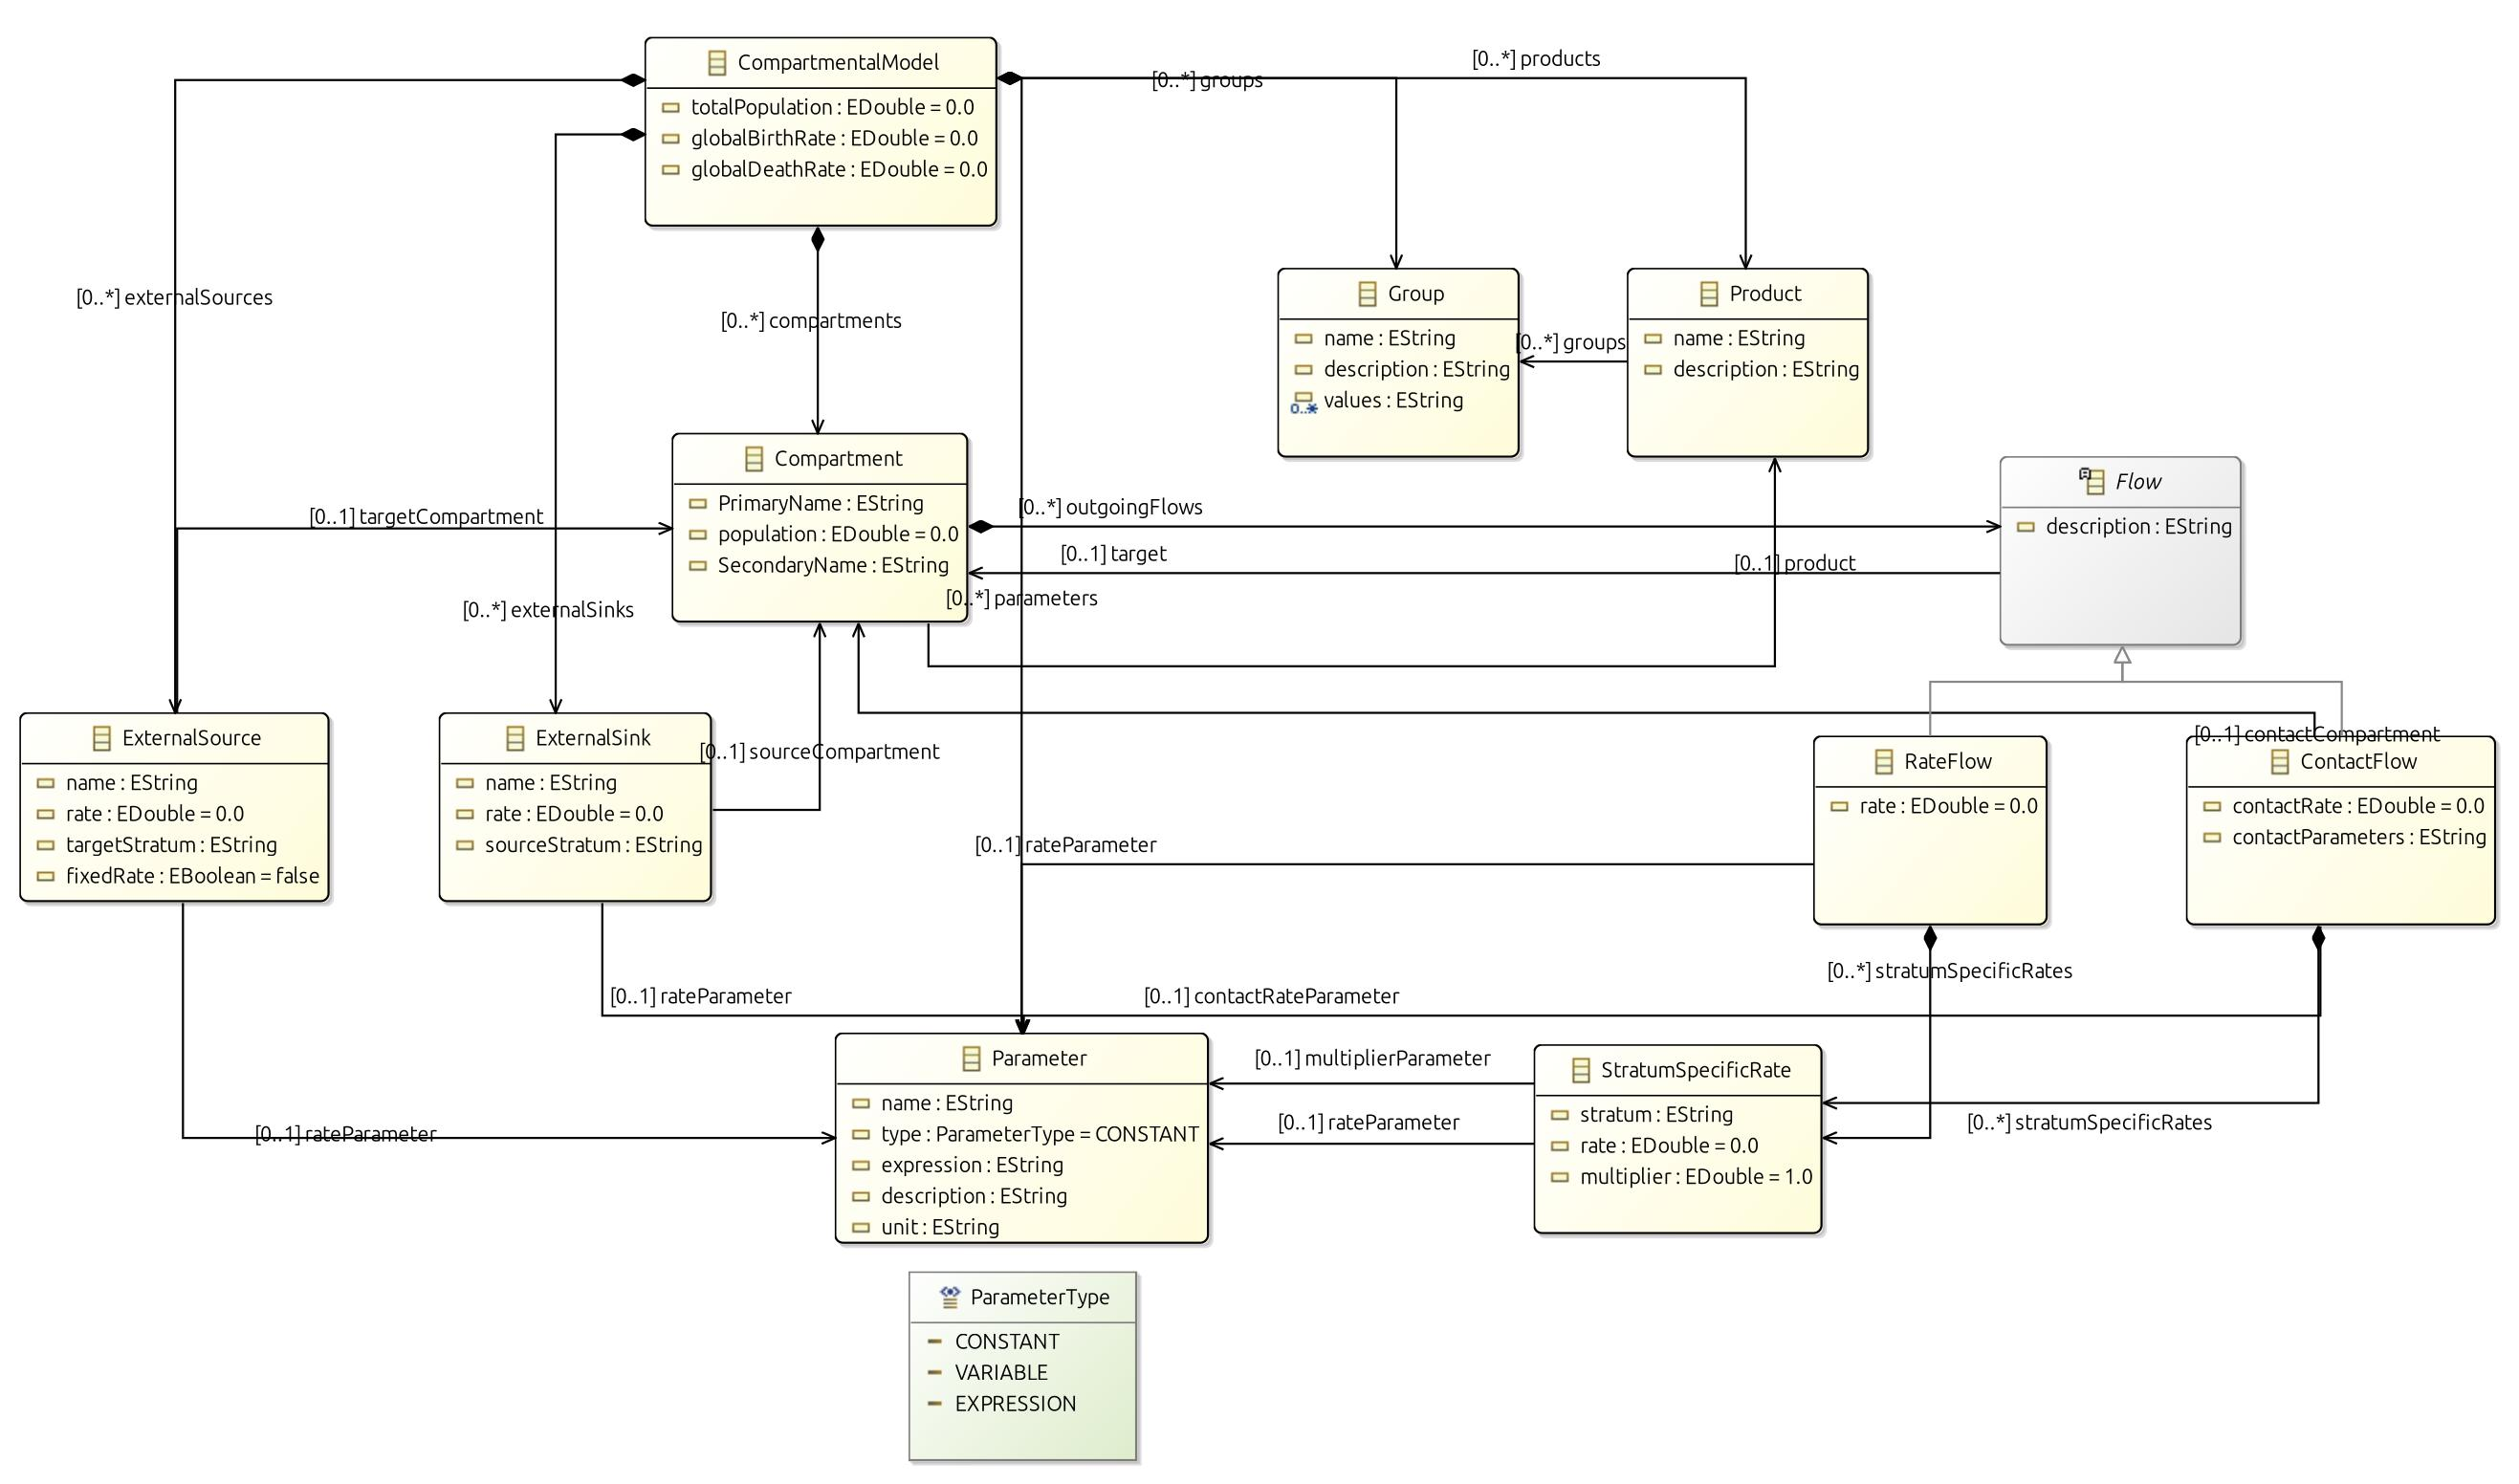
\includegraphics[width=\linewidth]{Figures/compartmentalmodel_classdiagram.jpg}
    \caption{The structure of the \texttt{EpiMDE-model} metamodel. The metamodel defines compartments, groups and products, as well as flows and simulation parameters.}
    \label{fig:compartmental_classdiagram}
\end{figure}

\texttt{EpiMDE-model} is using Sirius~\cite{viyovic2014sirius} to provide a graphical editor for its models and metamodels. The base metamodel declares the top level type $Epidemic$ as well as the $Compartment$ and $Flow$ types. An epidemic is composed of a single compartment, either a product or a group. The base $Compartment$ type is a unitary compartment class which generates a single physical compartment from its labels.



\paragraph{Groups and Products}

The group metamodel extension describes groups and products. A group is composed of any number of compartments and flows, and it extends the $Compartment$ class. Groups also reference some of their compartments as either $source$, $sink$, both or neither. Not all constraints can be seen in the metamodel diagram. For example, though a group could reference any compartment as its sink or source, the referenced compartments must be its direct children. Products are identical in structure to groups, except for the sources and sinks. Products derive their sources and sinks from the product of the sources and sinks of their children. Figure~\ref{fig:compartmental_classdiagram} shows the simplified implementation of Groups and Products, where stratification is represented directly without the compartment wrapper mechanism used in the extensible version for dynamic composition.



%\paragraph{Product}

%Figure \ref{fig:product_mm_graph} describes the product metamodel extension. 


%\begin{figure}[t]
%    \centering
%    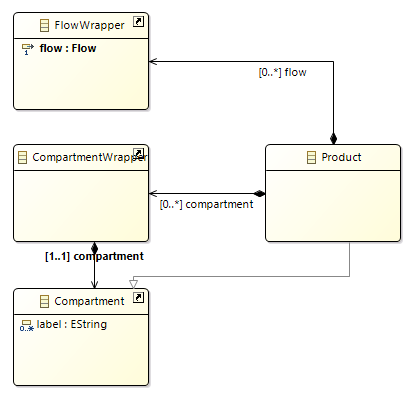
\includegraphics[width=0.6\linewidth]{Figures/product_mm_graph.png}
%    \caption{Product Metamodel}
%    \label{fig:product_mm_graph}
%\end{figure}

%Products are identical in structure to groups, except for the sources and sinks.
%Products derive their sources and sinks from the product of the sources and sinks of their children.
%The ability to place flows in products was not discussed and is not particularly important, it can be ignored.
%The idea is that a user could place an existing SEIR model in a product and add a flow from R to S, forming a typical SEIRS model.
%This could be done in groups too, not just products.
%Peeking inside a group from the outside is not necessarily good or bad, but is up for debate in future versions.


\paragraph{Basic Flows}
The basic flows extension provides the three basic types of flows: rates, batches and contacts. By making use of the class $FromToFlow$ in the hierarchy some functionalities common to all three flows are easily shared. Figure~\ref{fig:compartmental_classdiagram} shows a simplified subset of this extension, including $RateFlow$ and $ContactFlow$ types, which cover the most common epidemiological modeling scenarios, while the extensible version additionally includes batch flows for more specialized use cases.



\subsubsection{From metamodel extensions to models}

\begin{algorithm}[t]
\caption{Produce Physical Compartments of Group}
\label{alg:group}
\begin{algorithmic}
\Procedure{GetPhysicalCompartments}{}
\For{$wrapper \in this.getCompartment()$}
    \State $cmpt \gets wrapper.getCompartment()$ 
    \For{$pc \in cmpt.getPhysicalCompartments()$}
        \State $\textbf{yield} \: this.prependSelf(pc)$
    \EndFor
\EndFor
\EndProcedure
\end{algorithmic}
\end{algorithm}

\begin{algorithm}[t]
\caption{Produce Physical Compartments of Product}
\label{alg:product}
\begin{algorithmic}
\Procedure{GetPhysicalCompartments}{}
\State $\textbf{alias} \: PC \gets PhysicalCompartment$
\State $List$<$List$<$PC$\text{>}\text{>} $ \: dimensions \gets []$
\For{$wrapper \in this.getCompartment()$}
    \State $cmpt \gets wrapper.getCompartment()$
    \State $List$<$PC$>$ \: dim \gets cmpt.getPhysicalCompartments()$
    \State $dimensions.add(dimn)$
\EndFor
\State $List$<$List$<$PC$\text{>}\text{>} $\:prod \gets CartesianProduct(dimensions)$
\For{$List$<$PC$>$ \: pcs \in prod$}
    \State $PC \: pc \gets join(pcs)$
    \State $\textbf{yield} \: this.prependSelf(pc)$
\EndFor
\EndProcedure
\end{algorithmic}
\end{algorithm}

Given the extension mechanisms discussed previously, it becomes evident that the task of creating a model from the proposed metamodel is not a straightforward process. Normally, a metamodel would serve as the DSL that would guide the creation of models; it informs the modeler of what elements are available, how they can be connected, what properties they can have and what constraints govern their structure and relations. As we have mentioned, the metamodel extensions we propose here are based on abstract notions that before being used in concrete models they have to become concrete or ``physical'' as we call the resulting components. Thankfully, this process, which we will discuss here, is hidden from the modeler, who only sees the resulting DSL.

The processes for generating the physical components for $Groups$ and $Products$ are described in java-like pseudo code in Algorithms~\ref{alg:group} and~\ref{alg:product} respectively. Note that all $.getCompartment()$ methods are automatically generated by EMF from the compositions in the UML diagram being named $compartment$. The version for compartment wrappers returns a compartment while the group and product versions return $EList$ of compartment wrappers. $prependSelf$ is a utility to add the labels of the current compartment at the beginning of the labels list of the produced physical compartments.

\paragraph{Algorithm Explanation}

\textbf{Algorithm~\ref{alg:group} (Group Physical Compartments Generation)} transforms a Group's logical structure into its physical representation through a flattening process. The algorithm operates as follows:
\begin{enumerate}
    \item \textbf{Iterate through child compartments} (lines 2-3): For each compartment wrapper contained in the Group, extract the underlying compartment. This handles the EMF wrapper mechanism described in Section~\ref{sec:metamodel}.
    \item \textbf{Recursively expand children} (lines 4-5): Call $getPhysicalCompartments()$ on each child compartment. This recursive call handles nested Groups and Products, ensuring full expansion regardless of hierarchy depth.
    \item \textbf{Prepend Group label} (line 5): For each physical compartment produced by a child, prepend the current Group's label to create a hierarchical label path. For example, if Group ``Age'' contains compartment ``Child'', the physical compartment becomes ``Age-Child''.
    \item \textbf{Yield results} (line 5): Return each labeled physical compartment one at a time, enabling lazy evaluation for large stratifications.
\end{enumerate}
The algorithm's key insight is that Groups simply flatten their children while maintaining hierarchical labeling. If a Group contains 3 child compartments, it produces 3 physical compartments with prepended labels.

\textbf{Algorithm~\ref{alg:product} (Product Physical Compartments Generation)} implements Cartesian product logic to generate all stratum combinations. The algorithm proceeds as follows:
\begin{enumerate}
    \item \textbf{Collect dimensions} (lines 2-6): Iterate through all child compartments (each representing a stratification dimension), recursively expand each to physical compartments, and store the result as a dimension. For example, an age Group with 3 values and a sex Group with 2 values create two dimensions: $[[Age_1, Age_2, Age_3], [Sex_1, Sex_2]]$.
    \item \textbf{Compute Cartesian product} (line 7): Apply the mathematical Cartesian product operation to the list of dimensions. This generates all possible combinations: if dimensions have sizes $[n_1, n_2, ..., n_k]$, the product produces $n_1 \times n_2 \times ... \times n_k$ combinations. For the age-sex example, this produces 6 combinations: $(Age_1, Sex_1), (Age_1, Sex_2), (Age_2, Sex_1), ..., (Age_3, Sex_2)$.
    \item \textbf{Join labels} (lines 8-9): For each combination (a list of physical compartments), merge their labels into a single physical compartment. For example, $(Age_{20-64}, Location_A)$ becomes a single physical compartment with label $[Age, 20-64, Location, A]$.
    \item \textbf{Prepend Product label} (line 9): Add the Product's own label to the beginning of the merged label list, creating a complete hierarchical path.
    \item \textbf{Yield results} (line 9): Return each product physical compartment, enabling lazy evaluation.
\end{enumerate}
The algorithm's complexity is $O(n_1 \times n_2 \times ... \times n_k)$ where $n_i$ is the size of dimension $i$, which is inherent to the Cartesian product operation. In practice, Products typically have 2-3 dimensions with 2-5 values each, resulting in manageable expansion (e.g., $3 \times 2 = 6$ or $4 \times 3 \times 2 = 24$ physical compartments).



The algorithms to generate sources and sinks are quite similar. Groups gather the source physical compartments of its source compartments, while products produce the Cartesian product of the source physical compartments of their children. The algorithms used to gather equations are nearly identical. Algorithms used by flows to produce their physical representations rely on the parameterization patterns that were presented before.

\section{The EpiMDE IDE}
\label{sec:EpiMDE}

In this section, we outline the requirements for modeling platform in the context of compartmental models, and then we discuss the design and features of the proposed platform.

\subsection{Platform Requirements}

Understanding how and why epidemiologists will use our platform is the first step in order to design it.
With the help of an epidemiologist, we identified atomic use cases for our platform to support, presented as user stories in \autoref{t:requirements}.
\newcounter{requirementscounter}
\setcounter{requirementscounter}{1}

\begin{table*}[htbp]
\footnotesize
\caption{Infectious Disease Modeling User Stories.}
\label{t:requirements}
\begin{tabular}{l | p{4.2cm} p{7.2cm}}
\hline 
\multicolumn{3}{l}{As a modeler, I want to:}                   \\ \hline 
\ifnum\value{requirementscounter}<10 0\fi\arabic{requirementscounter} \stepcounter{requirementscounter} & create models. &                               \\
\ifnum\value{requirementscounter}<10 0\fi\arabic{requirementscounter} \stepcounter{requirementscounter} & store models, & to access them over time.     \\
\ifnum\value{requirementscounter}<10 0\fi\arabic{requirementscounter} \stepcounter{requirementscounter} & share models, & to collaborate with other modelers.\\
\ifnum\value{requirementscounter}<10 0\fi\arabic{requirementscounter} \stepcounter{requirementscounter} & compare models, & to automatically list differences.\\
\ifnum\value{requirementscounter}<10 0\fi\arabic{requirementscounter} \stepcounter{requirementscounter} & modify existing models, & to improve them.              \\
\ifnum\value{requirementscounter}<10 0\fi\arabic{requirementscounter} \stepcounter{requirementscounter} & add data sources to a model, & for the purpose of calibration. \\
\ifnum\value{requirementscounter}<10 0\fi\arabic{requirementscounter} \stepcounter{requirementscounter} & calibrate models, & to evaluate fitness of model results to available data. \\
\ifnum\value{requirementscounter}<10 0\fi\arabic{requirementscounter} \stepcounter{requirementscounter} & inspect the parameter values from calibration, & to verify/validate calibration results. \\
\ifnum\value{requirementscounter}<10 0\fi\arabic{requirementscounter} \stepcounter{requirementscounter} & simulate scenarios of interest, & to answer questions of analysts.\\
\ifnum\value{requirementscounter}<10 0\fi\arabic{requirementscounter} \stepcounter{requirementscounter} & make reports of scenario results, & to present to analysts.\\
\ifnum\value{requirementscounter}<10 0\fi\arabic{requirementscounter} \stepcounter{requirementscounter} & analyze the behavior of the model, &  to verify/validate scenario results (i.e. sensitivity analysis). \\
\ifnum\value{requirementscounter}<10 0\fi\arabic{requirementscounter} \stepcounter{requirementscounter} & recalibrate models, & to take into account updated data sources.  \\
\ifnum\value{requirementscounter}<10 0\fi\arabic{requirementscounter} \stepcounter{requirementscounter} & document the models (structure, parameters, calibrations, scenarios, results), & to make reports and/or publications. \\
\ifnum\value{requirementscounter}<10 0\fi\arabic{requirementscounter} \stepcounter{requirementscounter} & make use of metamodel extensions, & to simplify or accelerate the modeling task. \\
\hline 
\hline 
\multicolumn{3}{l}{As an analyst, I want to:}               \\ \hline 
\ifnum\value{requirementscounter}<10 0\fi\arabic{requirementscounter} \stepcounter{requirementscounter} & define scenarios of interest &                           \\
\ifnum\value{requirementscounter}<10 0\fi\arabic{requirementscounter} \stepcounter{requirementscounter} & consult scenario results or query new results by running new simulations & to answer research questions and inform public health policy. \\
\ifnum\value{requirementscounter}<10 0\fi\arabic{requirementscounter} \stepcounter{requirementscounter} & view the model's structure, parameters, and calibrations, & to elicit new scenarios and to ask questions about the model to modelers (e.g., flagging issues). \\
\hline 
\hline 
\multicolumn{3}{l}{As an auditor, I want to:}               \\ \hline 
\ifnum\value{requirementscounter}<10 0\fi\arabic{requirementscounter} \stepcounter{requirementscounter} & consult scenario results or query new results, & to understand the model's behavior and/or test the model.\\
\ifnum\value{requirementscounter}<10 0\fi\arabic{requirementscounter} \stepcounter{requirementscounter} & view the model's structure, parameters, and calibrations,  & to verify/validate the model. \\
\ifnum\value{requirementscounter}<10 0\fi\arabic{requirementscounter} \stepcounter{requirementscounter} & run a simulation, & to verify/validate reported results. \\
\ifnum\value{requirementscounter}<10 0\fi\arabic{requirementscounter} \stepcounter{requirementscounter} & review the documentation of the models & to understand their structure, parameters, calibrations, scenarios, and results. \\
\hline
\hline 
\multicolumn{3}{l}{As a metamodeler, I want to:}               \\ \hline 
\ifnum\value{requirementscounter}<10 0\fi\arabic{requirementscounter} \stepcounter{requirementscounter} & implement new types of equations, & to represent real-world behaviour of a disease or population.\\
\ifnum\value{requirementscounter}<10 0\fi\arabic{requirementscounter} \stepcounter{requirementscounter} & implement new types of compartments, & to represent an existing population classification.\\
\ifnum\value{requirementscounter}<10 0\fi\arabic{requirementscounter} \stepcounter{requirementscounter} & share my metamodel extensions, & to facilitate collaboration and reproducibility.\\
\hline
\end{tabular}%
%}
\end{table*} % todo this damn table better be inlined

In this paper, we focus on user stories 1-5, 14 and 20 for creating and managing epidemiological models, as well as 22, 23 and 24 which enable metamodeling for platform users. The current implementation of the platform also enables user stories 9, and 15-21.

We identify platform features required to fulfill the identified user stories:
\begin{itemize}
    \item Base metamodel type system \{1, 22, 23\}
    \item Graphical modeling interface for model creation \{1\} and modification \{5\}
    \item Model comparison \{4\}.
    \item Runtime metamodel extensibility using plugins \{14, 24\}
    \item Infer and enable simulations as derived from a model \{9,15-21\}
\end{itemize}

\subsection{Basic functionality}

The EpiMDE IDE offers the ability to create models based on the metamodel we proposed previously. Based on the Eclipse user interface, the modeler can choose to create a new EpiMDE project and start modeling. The project includes the basic model, which can be augmented with selected extensions. Extensions can be included in the project as Java libraries (JAR files). Through the ``New Project'' wizard, the modeler can choose all desired extensions. Once the project is created, the elements that are defined in the base metamodel and in the extensions will be come available to the modeler. 

The modeler is presented with a graphical interface and a graphical language to start creating the models. Compartments are represented using rectangles which contain flows and other compartments. Compartments and flows have their name and type displayed within their shape. Flows are not arrows, but rather diamonds with labeled arrows pointing from it to compartments. The reason for this is that a flow is not a simple relation between compartments, but a first class element with its own properties, including rates, sources, sinks and so on. Each line pointing from a flow to a compartment is labeled according to its role. For example, a contact $C$ has three arrows labeled "from", "to" and "contact" and on the diamond is displayed "Contact $C$".

The IDE inherits a lot of the features of the EMF graphical editors. As such, if an element, a compartment or a flow, is clicked, its properties are displayed and can be directly edited. The label is an example of such a property. For more details, extra options can be accessed. Groups, for example, offer a form of toggle for each of their children marking them as sink, source, neither or both. This is not visible as a property but rather requires opening it in a popup. In addition, the editor presents warnings for structural errors ``live'' during development. This prevents the generation of simulations, unless all errors are fixed. Possible errors may include removing references from a flow to a compartment and not pointing it to a new one, when removing all the labels from a compartment, or making use of the same labels twice on different compartments.


The graphical interface is made available using a Sirius\footnote{\url{https://eclipse.dev/sirius/overview.html}} viewpoint definition project. It allows us to define rules for presenting model element hierarchies and relationships. Specifically, we define two important rules, one for compartments and one for flows. Sirius allows recursive definitions using the $reused container mappings$ property, which we can apply to compartments so that their children compartments recursively display their children. A limitation from the combination of using Sirius and supporting open sets of types is that rendering types which are not compartments or flows is not supported. Our platform allows any model to be loaded, even if some elements are from an entirely different hierarchy. The Sirius viewpoint would not know how to display these objects, so they may only be accessible through properties of the object they belong to, through a popup implemented by the developer.

\subsection{Advanced functionalities}

Besides creating models, EpiMDE offers other modeling functions, including model comparison and differencing, parameterization, and simulation.

\subsubsection{Model Comparison}

Comparing models with their previous versions or with similar models helps detect errors and understand model behaviour. It is an important task to increase model reproducibility as it enables users to definitively know when two models present differences. For model versioning it accelerates common tasks such as merging or extracting commonalities.

For our purposes, model comparison operates at the structural level but provides information aggregating the physical representations produced by the model. In other words, if two models are different but produce the same representation, this will be clear to the user. Similarly, if two models are structurally identical but a property differs which yields a different physical representation, this will also be presented to the user. Metamodelers may find these features helpful in the event where they want to develop a metamodel extension. By creating a reference model which produces the desired output and comparing it with the result of a model making use of the extension, they can automatically validate the output of the extension.

The current implementation of model comparison identifies simple differences like renaming, adding and deleting, or compound differences like moves, which corresponding to deleting and adding the same element. We have built a domain-specific comparison algorithm on top of the EMF Compare\footnote{\url{https://eclipse.dev/emf/compare/}} and EMF DiffMerge\footnote{\url{https://wiki.eclipse.org/EMF_DiffMerge/}} frameworks. 

Model comparison relies on identifying a difference as either retyping, renaming, moving, adding or deleting, then synthesizing the differences for the user in their most useful form.
Some model difference patterns can be synthesized into more easily understood ones, such as presenting matching added and deleted elements as moves. New elements that are contributed by metamodel extensions need to override an abstract comparison method. The results of the comparison follow the hierarchical structure of the model components.

The model comparison comprises of two steps. In the first step (Algorithm~\ref{alg:match}), the elements of the two models to be compared are matched. Two elements are matched if they have identical labels or if they have the exact same contents. This allow us to match elements, even if they are renamed between the two models. When considering physical compartments, the lists of labels need to be identical.

\paragraph{Model Matching Algorithm Explanation}

\textbf{Algorithm~\ref{alg:match} (SameUniqueLabelMatch)} establishes correspondences between compartments in two models being compared. The algorithm uses label-based matching with hierarchical propagation:

\begin{enumerate}
    \item \textbf{Identify unique labels} (line 2): Compute the intersection of labels that appear exactly once in model 1 and exactly once in model 2. These unique labels serve as reliable anchors for matching. For example, if both models have exactly one compartment labeled ``Infectious-Symptomatic'', this label is unique and trustworthy for matching.

    \item \textbf{Match compartments by unique labels} (lines 4-10): For each pair of compartments $(c1, c2)$ from the two models, check three conditions: (a) $c1$ is not yet matched, (b) $c2$ is not yet matched, and (c) $c1$ and $c2$ share at least one unique label. If all conditions hold, create a match between $c1$ and $c2$. This ensures one-to-one matching using only reliable label evidence.

    \item \textbf{Propagate matches to parents} (lines 12-18): For each established match, examine the parent containers of the matched compartments. If both parents are compartments (e.g., Groups or Products), have the same type, and are not yet matched, create a parent match. This hierarchical propagation enables matching of aggregate structures based on their matched children. For example, if all children of two Groups are matched, the Groups themselves should be matched.

    \item \textbf{Return match result} (line 20): The algorithm produces a MatchResult containing pairs of corresponding elements, establishing the basis for subsequent difference detection.
\end{enumerate}

The algorithm's strength lies in its use of unique labels as anchors combined with hierarchical propagation, enabling robust matching even when models have been partially restructured or renamed. 


\begin{algorithm}[th]
\caption{SameUniqueLabelMatch}
\label{alg:match}
\begin{algorithmic}
\State $res \gets$ new MatchResult()
\State $uniqueLabels \gets$ $intersection$(unique labels of model 1, unique labels of model 2)

\For{$each$ $Compartment$ $c1$ $\in$ model 1}
    \For{$each$ $Compartment$ $c2$ $\in$ model 2}
        \If{$res$.$find$($c1$) is empty \textbf{and} $res$.$find$($c2$) is empty \textbf{and} $intersection$($c1$.$labels$, $c2$.$labels$, $uniqueLabels$).$size$() > 0}
            \State Add $Match$($c1$, $c2$) to $res$
        \EndIf
    \EndFor
\EndFor

\For{$each$ $Match$ $match$ $\in$ $res$.$matches$}
    \State $leftParent \gets m.left.eContainer()$
    \State $rightParent \gets m.right.eContainer()$
    \If{$leftParent$ is a $Compartment$ \textbf{and} $leftParent$ same class as $rightParent$ \textbf{and} $leftParent$ not matched \textbf{and} $rightParent$ not matched}
        \State Add $Match$($leftParent$, $rightParent$) to $res$
    \EndIf
\EndFor

\State \textbf{Return} res
\end{algorithmic}
\end{algorithm}

In the second step of the comparison (Algorithm~\ref{alg:differencing}), matched elements are compared to find differences. Each pair of matched compartments is compared, but since aggregate compartments of the same type compare their children, they are marked as \emph{accounted for} and synthesized as part of their parent comparison. The partial ordering produced by the matching algorithm allows us to iterate directly through matches and always find a parent match before their children, enabling the \emph{accounted for} process.
Once the differencing is done, moves are also synthesized using matching additions and subtractions.

\paragraph{Differencing Algorithm Explanation}

\textbf{Algorithm~\ref{alg:differencing} (Differencing)} computes structural differences between matched model elements and synthesizes high-level change operations. The algorithm works as follows:

\begin{enumerate}
    \item \textbf{Initialize with root comparison} (lines 1-2): Begin by comparing the first matched pair (typically the root models). This produces an initial set of differences (additions, deletions, modifications) and marks compared elements as ``accounted for''.

    \item \textbf{Compare remaining matches} (lines 4-7): Iterate through all remaining matched pairs. For each match not yet accounted for (i.e., not already compared as part of a parent's comparison), invoke the $compare$ method to identify differences. The ``accounted for'' check prevents redundant comparisons---if a Group's children were already compared recursively during the Group comparison, they are skipped here.

    \item \textbf{Synthesize moves from additions and deletions} (lines 8-15): Examine all differences identified as additions. For each added compartment $c$, check if $c$ appears in the match set (meaning it exists in both models but in different locations). If so, reclassify the addition-deletion pair as a \textit{move} operation rather than separate add and delete operations. This provides more intuitive change descriptions---``compartment X moved from Group A to Group B'' is clearer than ``X deleted from A and X added to B''.

    \item \textbf{Return synthesized differences} (line 16): The final result is a set of high-level differences (additions, deletions, modifications, moves) that accurately describe model evolution.
\end{enumerate}

The algorithm's key contribution is synthesizing low-level structural changes (add/delete) into semantically meaningful operations (move), making comparison results easier for modelers to understand and act upon. The ``accounted for'' mechanism ensures efficient processing by avoiding redundant comparisons in hierarchical structures.


\begin{algorithm}[th]
\caption{Differencing}
\label{alg:differencing}
\begin{algorithmic}
\State $firstMatch \gets$ first match in $matches$
\State $diffs \gets$ \{$firstMatch.first$.compare($firstMatch.second$)\}

\For{$each$ $Match$ $match$ $\in$ $matches$}
    \If{$match$ not yet accounted for}
        \State $diffs$.$add$($match.first$.$compare$($match.second$))
    \EndIf
\EndFor
\For{$each$ $Difference$ $d$ $\in$ $diffs$}
    \For{$each$ $Compartment$ $c$ $\in$ $d$.$additions$}
        \If{$c$ is matched}
            \State Set match as move
        \EndIf
    \EndFor
\EndFor
\State \textbf{Return} $diffs$
\end{algorithmic}
\end{algorithm}



\subsubsection{Simulation}

Simulation refers to the application of equations over time, making use of equations, parameters and a scenario. Typically it is used to generate graphs used for estimating hospitalization, mortality, peak cases, etc. The output of a simulation are values for each compartment at every time step. A single simulation can then be used to produce multiple graphs of different aspects. The equations can be directly generated from the model, while parameterization of the equations and specification of scenarios happen separately, as will be described next. 

Before the simulation, a compilation phase where the equations are parsed and used to generate python functions is performed. Even though compilation can be computationally expensive, it only needs to happen once for every model. Each equation will be evaluated thousands of times during simulation, so any time lost to compilation can be repaid many times over by saving simulation time. The compilation phase applies some simple optimizations. For example, compartments are placed into an array, making use of indices rather than labels for accessing the values. Similarly for parameters, where the corresponding value is found during compilation in the parameterization file and inlined in the equation for simulation.

To simulate, all the user needs to do is specify a time span, a set of points in time the simulation will provide values for. This time series does not require regular steps and the steps do not necessarily dictate simulation detail. For example, the user may ask for daily steps for a year, followed by weekly steps for 4 years, but the simulation will step multiple times per day independently of the time span, in order to produce accurate results.

Simulation uses an ODE solver, such as the Fourth Order Runge-Kutta method, or approximates by making use only of the current derivative at a given time. The accuracy increases by making use of higher order derivatives instead of only the first derivative, at the cost of increased simulation time. The current simulation environment supports both approaches with a toggle. According to our experiments, for a model with a large amount of compartments, the cost of using an ODE is too large. Population changes to any compartment value affects hundreds of equations, leading to confusion for the ODE as to the evaluation of the higher order derivatives, which makes it collapse for very short time steps. The current implementation makes use of a very naive approach in which the user provides a tolerance which each compartment change between two steps must conform. If the tolerance is not reached between a step from $t_1$ to $t_2$, we recursively call the simulation with 10 steps [$t_1$, $t_1 + 0.1 * t_2$, ...,  $t_1 + 0.9 * t_2$, $t_2$], which may or may not further divide the steps based on tolerance. Finally, we offer a functionality to plot values easily by using the labels found in the model. For example, $plot\_by\_labels$([[$'Alive'$], [$'Deceased'$]], [$'I-TB'$]) plots two curves: $Alive$ and $Deceased$, for all $I-TB$, compartments of people infected with tuberculosis.

\paragraph{Scenarios}
A scenario is a distribution of the population in compartments at the beginning of a simulation.
For example, a Covid-19 simulation for Canada requires a scenario with around 38 million people placed in the compartments, while a simulation for the united states requires around 330 million, but also the age and comorbidities distributions.
Much of the code for scenarios is specific to the geographical area of the studied population, unlike parameters in equations.

\paragraph{Parameterization}

In order to use a model for simulation, it is necessary for the user to provide values for each equation parameter and original compartment population. Our solution offers parameterization in the same environment as the simulation, in a python notebook. This enables a very short feedback loop between verifying a model behaviour in the simulation and making changes to the parameters.

Equations inside products with many dimensions produce a large amount of parameters that are likely closely related. Our solution offers an API for selecting parameters using operand criteria to set all relevant instances at once by providing a tensor of values. Generic python functions for manipulating parameters and scenario values allow for parameterizing a model in a reasonable time. If a parameterization call is invalid it is flagged right away, such as providing an incorrect amount of values for a selection of parameters.

Parameters always have at least 2 arguments, the first is their name, such as $contact-mixing$ and the second is the name of the equation they are used in. More arguments are required to differentiate parameters used in variations of an equation, such as contacts between different age groups for example. Specifically for the contact, the third argument is the source compartment and the fourth is the contact compartment.

\subsection{AI-powered generation of disease models and simulations}

A key barrier to adopting model-driven approaches in epidemiology is the learning curve associated with metamodel concepts and XML-based model specifications. Even though EpiMDE simplifies modeling through graphical interfaces, epidemiologists still need to learn the modeling environment and understand metamodel constraints. To address this, we developed a multi-stage LLM (Large Language Model) pipeline that automatically generates EpiMDE-compatible models from plain-text specifications, transforming human-readable disease descriptions into executable simulation code.

The pipeline accepts as input (a) structured textual specifications written in plain English and (b) the \texttt{EpiMDE-model} specification from Section~\ref{sec:metamodel}. It produces complete XML model files conforming to the metamodel, which can be directly imported into the EpiMDE IDE for visualization, validation, and simulation. This approach eliminates the need for users to manually author XML or learn the graphical modeling interface, making epidemiological modeling accessible to researchers who prefer working with textual descriptions.

\subsubsection{Pipeline Architecture}

The LLM-based pipeline consists of three stages, each addressing a specific aspect of model generation:

\textbf{Stage 1 (Structural XML Generation):} The first stage generates structurally correct XML conforming to the \texttt{EpiMDE-model} from user-provided textual specifications. Users organize epidemiological information into plain-text instructions without requiring XML syntax knowledge. The input includes:

\begin{itemize}
    \item \textit{Model Type Declaration}: Specifying parametric modeling (using symbolic parameter names with Greek letters, recommended for published models) or numeric modeling (with hardcoded values).
    \item \textit{Compartment Structure}: Listing base compartments with primary and secondary names, including stratification product references when applicable.
    \item \textit{Stratification Specification}: Defining Groups and Products as described in Section~\ref{sec:metamodel}.
    \item \textit{Parameters Table}: Documenting parameter names (supporting Unicode Greek symbols like $\beta$, $\gamma$, $\mu$ and subscripts), types (CONSTANT, VARIABLE, EXPRESSION), values or expressions, descriptions, and units.
    \item \textit{Flow Specification}: Describing transitions with flow type (RateFlow/ContactFlow), source and target compartments, rate parameter references or expressions, and optional stratum-specific rates.
    \item \textit{Birth and Death Sources}: Specifying population dynamics with rate parameters and compartment or stratum targets.
    \item \textit{Initial Populations}: Providing starting distributions across compartments and strata.
\end{itemize}

Critically, users do not need to provide visual diagrams. This eliminates ambiguity between visual representations and declarative specifications, making the textual input the single source of truth and reducing LLM misinterpretation risk. No specific structure for the input is expected as long as the aforementioned elements are present.

The LLM receives these specifications along with the metamodel definition and generates XML with proper element names, attributes, nesting, and namespaces. For parametric models, it creates \texttt{<parameters>} elements with symbolic names and references them in flows using metamodel-compliant pointer syntax (\texttt{//@parameters.X}). For numeric models, it uses placeholder values that are filled in Stage 2. The LLM includes reasoning via XML comments explaining compartment counts, stratification mappings, flow interpretations, and assumptions, providing transparency for validation.

\textbf{Stage 2 (Value Mapping and Verification):} For parametric models, Stage 2 performs minimal verification, confirming that parameter definitions match flow requirements and references are correctly formed. For numeric models, Stage 2 maps rate values from user input to XML placeholders.

A critical design constraint is that the LLM performs \textit{no calculations}. It locates numeric values explicitly provided in user input and copies them to appropriate XML locations. This eliminates LLM misinterpretation of mathematical expressions by moving all mathematical decisions to user input preparation, ensuring reproducibility through explicit numerical specifications. The LLM documents each modification via XML comments, maintaining full numerical precision without structural changes.

\textbf{Stage 3 (Simulation Script Generation):} Stage 3 converts the EpiMDE model's Ordinary Differential Equations (ODE) (automatically generated by the platform as described in Section~\ref{sec:EpiMDE}) into executable Python code using a two-phase approach that separates structural setup from mathematical logic.

\textit{Stage 3A (Setup and Structure)} fills structural components of a pre-written skeleton, handling variable declarations outside the integration loop. The LLM extracts compartment names from ODEs, converts them to valid Python identifiers, assigns initial populations, and creates history arrays for tracking simulation results. This low-risk phase involves only declarations, enabling error isolation.

\textit{Stage 3B (Simulation Logi)} completes the simulation using validated variable names from Stage 3A. The LLM converts ODEs to Python by extracting right-hand sides and preserving mathematical operations, generates Euler method updates with non-negativity enforcement, implements history recording, and creates plotting commands with human-readable labels.

The pre-written skeleton provides universal components (imports, user interaction, loop structure, plotting setup) that are common across all simulations. Pre-writing these eliminates formatting inconsistencies and focuses the LLM on model-specific code. Both phases mandate raw Python code only (no markdown or code fences) ensuring direct executability.

\subsubsection{Key Design Principles}

The pipeline architecture embodies several important design principles that enhance reliability and usability:

\textbf{Separation of Concerns.} Each stage addresses a distinct aspect of model generation (structure, parameter/values, simulation), enabling targeted validation and error localization. If simulation fails, the problem can be traced to a specific stage rather than requiring regeneration of the entire pipeline.

\textbf{Explicit Reasoning Through Comments.} XML and Python comments document the LLM's reasoning at each decision point, creating transparent audit trails. This allows epidemiologists to verify that their specifications were correctly interpreted without understanding the underlying metamodel or code generation mechanics.

\textbf{Reproducibility.} The pipeline maintains interaction logs and uses deterministic value mapping (no implicit calculations), ensuring that the same textual specification always produces the same model. This addresses the reproducibility challenges identified in Section~\ref{sec1}.

\textbf{Parametric versus Numeric Modeling.} Supporting both parametric (symbolic equations with Greek letters matching published notation) and numeric (immediate executable models) approaches accommodates different use cases. Parametric models facilitate communication with the broader epidemiological community through familiar mathematical notation, while numeric models enable rapid prototyping and exploration.

\subsubsection{Advantages and Applicability}

The LLM-based pipeline offers several advantages that complement the manual modeling approaches demonstrated in previous case studies:

\textit{Accessibility for Non-MDE Experts.} Epidemiologists can specify models using familiar epidemiological terminology without learning the EpiMDE IDE or XML syntax. This dramatically lowers the barrier to entry compared to traditional MDE approaches.

\textit{Reduced Cognitive Load.} Textual specifications are often more concise than graphical model construction for complex stratified models. For instance, describing a 16-age-group COVID-19 model requires listing the stratification once in text, whereas graphical construction involves creating multiple interconnected elements.

\textit{Integration with Published Literature.} Parametric modeling with symbolic Greek letter notation enables direct transcription from published papers, reducing transcription errors and facilitating model reproduction from literature.

\textit{Automated Validation Through Metamodel Conformance.} The generated XML must conform to the metamodel, providing structural validation that manual text-based modeling approaches lack. Errors are caught at generation time rather than during simulation.

However, the pipeline also has limitations that must be acknowledged:

\textit{Dependency on LLM Accuracy.} While the structured prompt engineering and multi-stage design reduce errors, LLM outputs require careful validation. The pipeline is best viewed as an assistive technology that accelerates modeling rather than a fully autonomous system.

\textit{Manual Input Preparation.} Complex models require careful preparation of textual specifications, particularly for stratum-specific rates and intricate flow patterns. However, this is generally less error-prone than manual XML authoring.

\textit{Lack of Semantic Verification.} The pipeline enforces structural constraints (valid XML, correct references) but cannot detect implausible parameter combinations or epidemiologically invalid model structures. Domain expertise remains essential for validation.

\textit{Limited Support for Interactive Refinement.} The current implementation generates models in a single pass. Iterative refinement based on simulation results requires manual editing of the textual specification or switching to the graphical IDE.

\subsubsection{Comparison to Manual Modeling Workflows}

The LLM pipeline represents a complementary approach to the manual graphical modeling demonstrated in Case Studies 1-2. The graphical IDE excels when:
\begin{itemize}
    \item Modelers need visual understanding of model structure and flow patterns
    \item Exploratory modeling requires frequent structural changes
    \item Model composition and reuse leverage existing graphical models
    \item Domain experts prefer direct manipulation of model elements
\end{itemize}

The LLM pipeline excels when:
\begin{itemize}
    \item Models are being reproduced from published textual descriptions
    \item Modelers prefer working with mathematical notation over graphical representations
    \item Rapid generation of multiple model variants is needed for sensitivity analysis
    \item Accessibility considerations favor text-based interfaces over graphical tools
\end{itemize}

Importantly, the two approaches are not mutually exclusive. Models generated via the LLM pipeline can be loaded into the graphical IDE for visualization, refinement, and composition with other models. This hybrid workflow combines the accessibility benefits of automated generation with the interactive capabilities of graphical modeling.

\subsubsection{Evaluation of the automated model generation}

We evaluated the LLM pipeline by generating EpiMDE models for the HIV and COVID-19 case studies described in Sections~\ref{sec:casestudy:hiv} and~\ref{sec:casestudy:covid}. These models represent distinct epidemiological challenges, HIV with behavioral stratification and heterogeneous contact patterns, COVID-19 with age stratification and complex disease progression—enabling systematic assessment of the pipeline's generalizability. The pipeline was executed using two state-of-the-art LLMs: GPT-4o (OpenAI's gpt-4o model, temperature=0.7) and Gemini 2.5 Pro (Google, December 2024 release), enabling cross-model comparison of generation quality.

\textbf{Evaluation Methodology:} For Stages 1 and 2 (XML generation and value mapping), we employed element-level counting to assess model correctness. Each generated \texttt{.seirmodel} file (the specialized file of the EpiMDE platform) was parsed and its elements (compartments, parameters, flows, groups, products, sources, sinks) compared against ground truth specifications. Elements were classified as True Positives (correctly generated with accurate attributes), False Positives (hallucinated or incorrect elements), and False Negatives (specified but missing or incorrectly generated). From these counts, we calculated Precision = TP/(TP+FP), Recall = TP/(TP+FN), and F1 Score (harmonic mean). For Stage 3 (simulation scripts), we evaluated through manual code inspection and successful execution, verifying scripts ran without errors and produced expected outputs.


\section{Case Studies and Evaluation}
\label{sec:study}

In this section, we show how the platform can be used for simple or more complex modeling tasks. We present three case studies, one for modeling HIV, another for modeling COVID-19 and a third on rapid prototyping of epidemiological models. In the first two case studies, we attempt to replicate existing modeling works and demonstrate how our platform can achieve the same results, both from a structural and a simulation results perspective, while minimizing effort, thanks to the concise metamodel, the integrated platform and the use of generative AI. In both case studies, the assumption is that the modelers attempt to model a disease from a clean slate, i.e., they cannot or do not have prior models to reuse. We demonstrate how the modelers can use either the basic or the extensible metamodels to model the disease and use its tools to automatically generate and run simulation scenarios. In the third case study, we assume that the modeler intends to model a completely new disease, but this time by trying to reuse existing models or parts of existing models.

\subsection{Case Study 1: HIV Modeling}
\label{sec:casestudy:hiv}

In the first case study, we demonstrate how EpiMDE can be used to model a complex disease like HIV that also involves contact infections through sexual relationships. We replicate the model that was originally proposed by Espitia et al. (2022)\cite{Espitia2022}. This model categorizes the population into susceptible and untreated infectious groups across three distinct demographic subgroups: ``heterosexual men'', ``homosexual men''\footnote{We replicate the model by Espitia et al., which accounts for bisexual behavior through cross-group interactions (e.g., between ``homosexual men'' and ``women''), though it does not model bisexual or nonbinary individuals as separate demographic categories. This abstraction is common in mathematical epidemiology, but it necessarily simplifies the diversity of LGBT+ identities.}, and ``women''. Transitions between susceptible and infectious states are governed by contact-based transmission rates specific to each subgroup. Given that EpiMDE aims for simplicity and fast modeling, contact flows are modeled with basic flows, with rates estimated manually or from relevant literature, and as presented in the original publication.

Patients transition from untreated infectious states to either a \textit{Treated with ART} state or a \textit{People Living with AIDS (PLWA)} state. These compartments are shared across all genders consistent with the original model. The PLWA compartment ultimately leads to \textit{Death due to AIDS}, while all compartments except this terminal state flow into a \textit{Natural Death} compartment. All transitions, apart from contact-dependent flows, were modeled using explicit rate parameters derived from literature.


\subsubsection{Model Implementation in EpiMDE}

The model was implemented using EpiMDE's stratification features. First, a Group called "SexualBehavior" was defined with three values: "Homosexual Men", "Women", and "Heterosexual Men". A Product referencing this group was then created to enable automatic expansion of compartments across all three demographic strata. Next, compartments representing disease states (Susceptible, Infectious-Untreated, Treated with ART, Living with AIDS, HIV Deaths) were defined and associated with the Product, allowing each compartment to automatically represent all three demographic subgroups. This stratification approach demonstrates EpiMDE's capability to handle population heterogeneity efficiently, avoiding the need to manually create separate compartments for each combination of disease state and demographic group.

Subsequently, flows were defined to capture disease dynamics. ContactFlows with stratum-specific rates modeled HIV transmission through sexual contact, while RateFlows represented disease progression (e.g., from untreated to treated states, or progression to AIDS). The model also utilized ExternalSources to represent demographic recruitment into each subgroup and ExternalSinks to model natural mortality. Stratum-specific rates were employed throughout to capture heterogeneity in transmission, treatment, and demographic parameters across the three populations. To enhance visual distinction among subgroups, a color-based compartment border grouping was developed. Figure~\ref{fig:hiv_model} shows the stratified model for the women subgroup as an example; separate diagrams were generated for heterosexual men and homosexual men subgroups, each maintaining the same structure but with group-specific parameter values. Visually, the EpiMDE model is equivalent to the model in the original publication, but was constructed in a structured, disciplined (with preconditions, postconditions and constraints imposed) and replicable manner.

\begin{figure}[htbp]
    \centering
    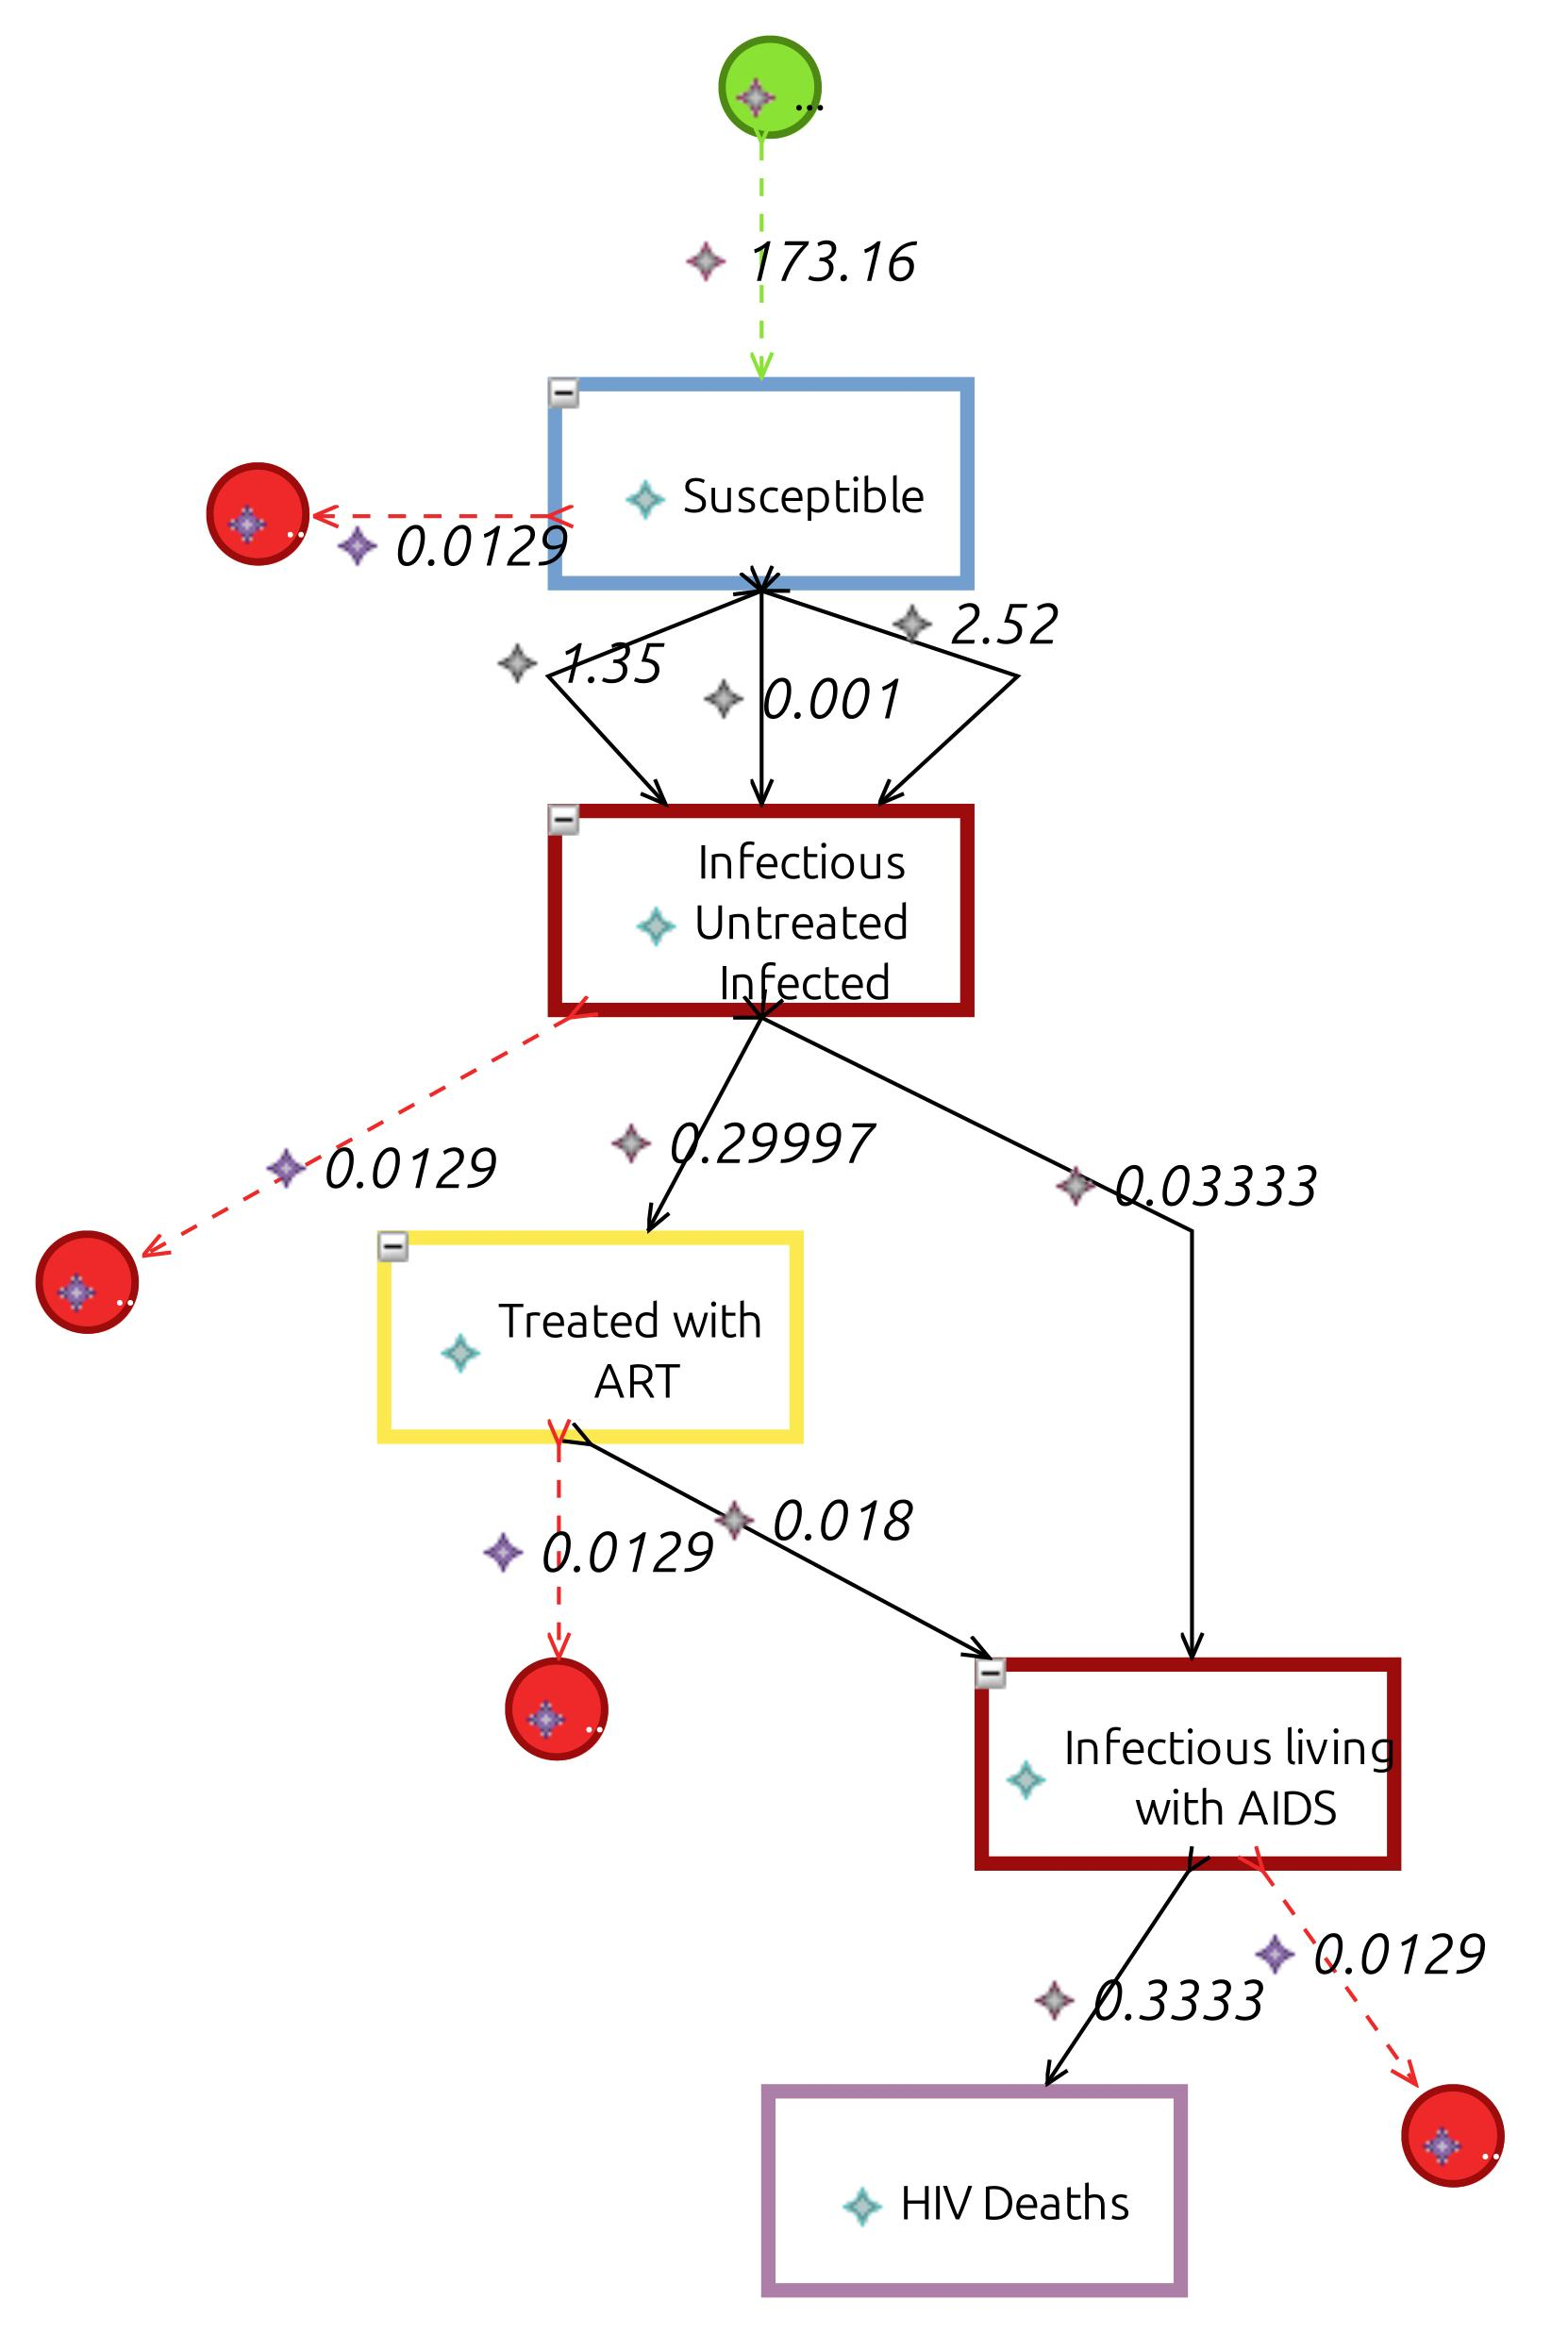
\includegraphics[width=0.5\textwidth]{Figures/HIV_Women.jpg}
    \caption{Graphical representation of the HIV-SEIR model in EpiMDE for the women demographic subgroup. Separate stratified diagrams exist for heterosexual men and homosexual men subgroups, maintaining the same compartmental structure.}
    \label{fig:hiv_model}
\end{figure}



\subsubsection{Simulation Automation}

Differential equations describing compartmental dynamics were automatically generated from the graphical representation, providing a robust mathematical foundation for simulations.

A Python script was developed to automate the simulation input process, enhancing usability by streamlining the following steps:
\begin{enumerate}
    \item Reading automatically generated .txt files containing differential equations.
    \item Guiding the user to select compartments for simulation.
    \item Collecting initial population sizes for each compartment.
    \item Specifying the simulation duration.
    \item Generating simulation outputs in .csv format, compatible with Excel or Google Sheets for further analysis.
\end{enumerate}
The results of the simulation were identical to those presented in the original publication showing the correctness and completeness of our model.



\subsubsection{LLM-Based Automated Generation Results}



To evaluate the LLM pipeline's capability to automatically generate the HIV model from textual specifications, we provided structured plain-text descriptions of the model's compartments, parameters, flows, and stratification structure to both GPT-4o and Gemini 2.5 Pro. The specification contained 66 total elements including compartments with behavioral stratification (sexual behavior groups), contact-based and rate-based flows, demographic sources and sinks, and stratum-specific transmission parameters.

\begin{table}[htbp]
\centering
\caption{LLM Performance for HIV Model Generation}
\label{tab:hiv_llm_performance}
\begin{tabular}{lccc}
\hline
\textbf{LLM Model} & \textbf{Precision} & \textbf{Recall} & \textbf{F1 Score} \\
\hline
GPT-4o & 86.4\% & 86.4\% & 0.864 \\
Gemini 2.5 Pro & 83.3\% & 100\% & 0.909 \\
\hline
\end{tabular}
\end{table}

\textbf{GPT-4o Performance:} The pipeline achieved balanced performance with Precision = 86.4\%, Recall = 86.4\%, and F1 = 0.864. All core structural elements were correctly generated: compartments with proper stratification references, the Group-Product structure for behavioral stratification, all 23 parameters with Unicode Greek letters and subscripts preserved, and birth/death sources with correct stratum assignments. The 9 false negatives and 9 false positives were primarily attributable to indexing errors in flow references—the LLM occasionally generated incorrect 0-based indices for \texttt{target} and \texttt{rateParameter} attributes. Critically, the structural integrity of the model was preserved; only specific numerical index values in flow references were incorrect. The generated simulation script (Stage 3) executed successfully, producing time-series plots for all stratified compartments with consistent variable naming and no runtime errors.

\textbf{Gemini 2.5 Pro Performance:} This model achieved perfect recall (100\%) but lower precision (83.3\%), yielding F1 = 0.909. Unlike GPT-4o, Gemini generated all 66 required elements with no omissions, demonstrating superior completeness. The 11 false positives consisted of indexing errors similar to GPT-4o and placeholder value hallucinations where the model inserted \texttt{rate="0.0"} attributes in parametric flows despite user input specifying only parameter references. This represents the LLM filling perceived specification gaps based on external modeling knowledge rather than strict input adherence. The simulation script generation succeeded with semantically organized code that grouped compartments by population, improving human readability.

\textbf{Key Findings:} Both models successfully captured the HIV model's core challenge—behavioral stratification with heterogeneous contact patterns—though with different error profiles. GPT-4o balanced precision and recall through conservative generation, while Gemini optimized for completeness at the cost of over-generation. The indexing errors shared by both models highlight a fundamental LLM limitation in tracking numerical references across many elements, suggesting the need for post-processing validation or intermediate index mapping steps. The perfect simulation script execution by both models validates the two-phase skeleton approach for code generation.

\subsection{Case Study 2: COVID-19}
\label{sec:casestudy:covid}

In our second case study, we demonstrate the use of the basic and extensible metamodels and of the modeling platform in the context of COVID-19 modeling. More specifically, we took the work of Tuite et al.~\cite{TuiteE497} on the mathematical modeling of COVID-19 transmission and mitigation strategies and we replicated the presented model using the proposed metamodel and modeling platform. We show how we can reach the same simulation results with a much reduced cognitive load, and a more concise and easier to understand model.

\subsubsection{Original model}

Figure \ref{fig:tuite1} displays the original figure from the article, Model structure of COVID-19 transmission\cite[Figure~1]{TuiteE497}. Further information in the article notes that this model is stratified along sixteen age groups as well as presence and absence of comorbidity, which will be used in equations but are absent in the graphical notation. The stratifications used by the researchers are a consequence of their available data. The population age data uses 20 intervals of 5 years and one for 100 years old or older. The contact mixing data uses 14 intervals of 5 years and one for 70 or older.

It is important to note that important information about the model was not possible to be extracted just from the manuscript, but part of it was extracted by further investigating the accompanying source code repository. This further emphasizes the need to gather all model elements under a single location to improve communication and reproducibility.

\begin{figure}[t]
    \centering
    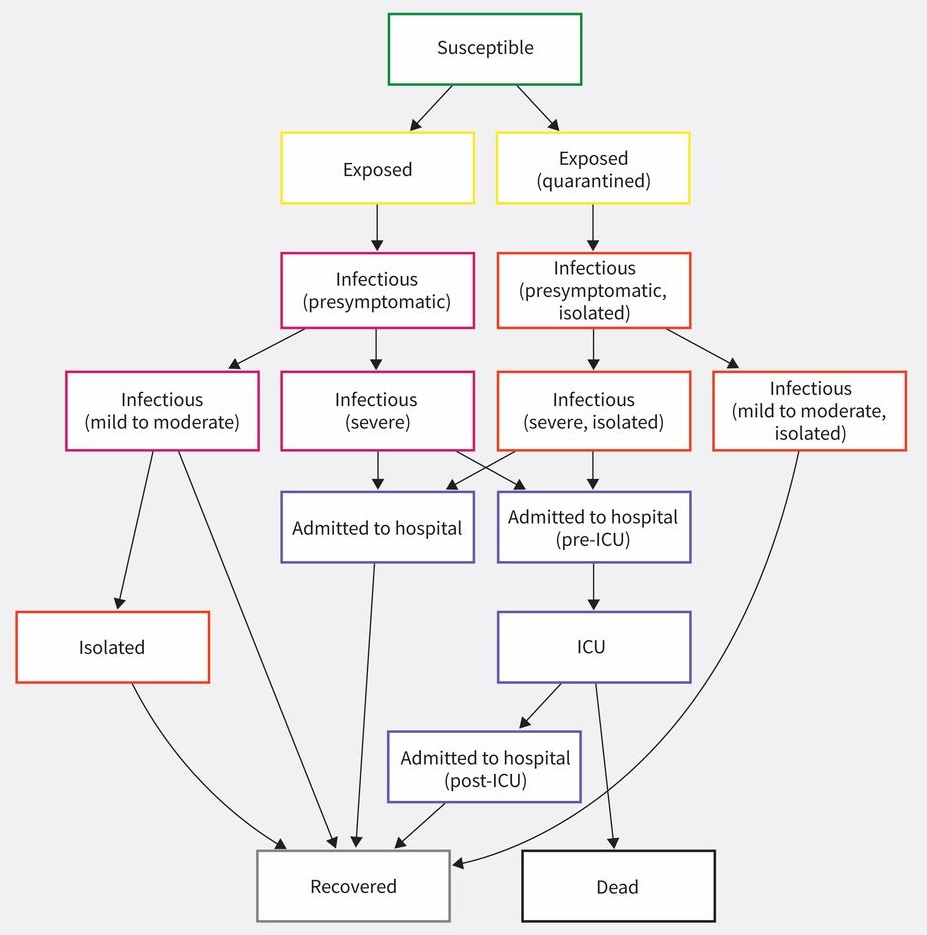
\includegraphics[width=\linewidth]{Figures/tuite1.jpg}
    \caption{Original COVID-19 Model Representation~\cite{TuiteE497}}
    \label{fig:tuite1}
\end{figure}



\subsubsection{Translated model}

In order to represent the disease model in our platform, present two approaches: using the basic metamodel (EpiMDE) and the extensible metamodel. As it can be seen in Figure~\ref{fig:covid_model}, the generated EpiMDE model is almost identical to the original model (Figure~\ref{fig:tuite1}).

\begin{figure}[htbp]
    \centering
    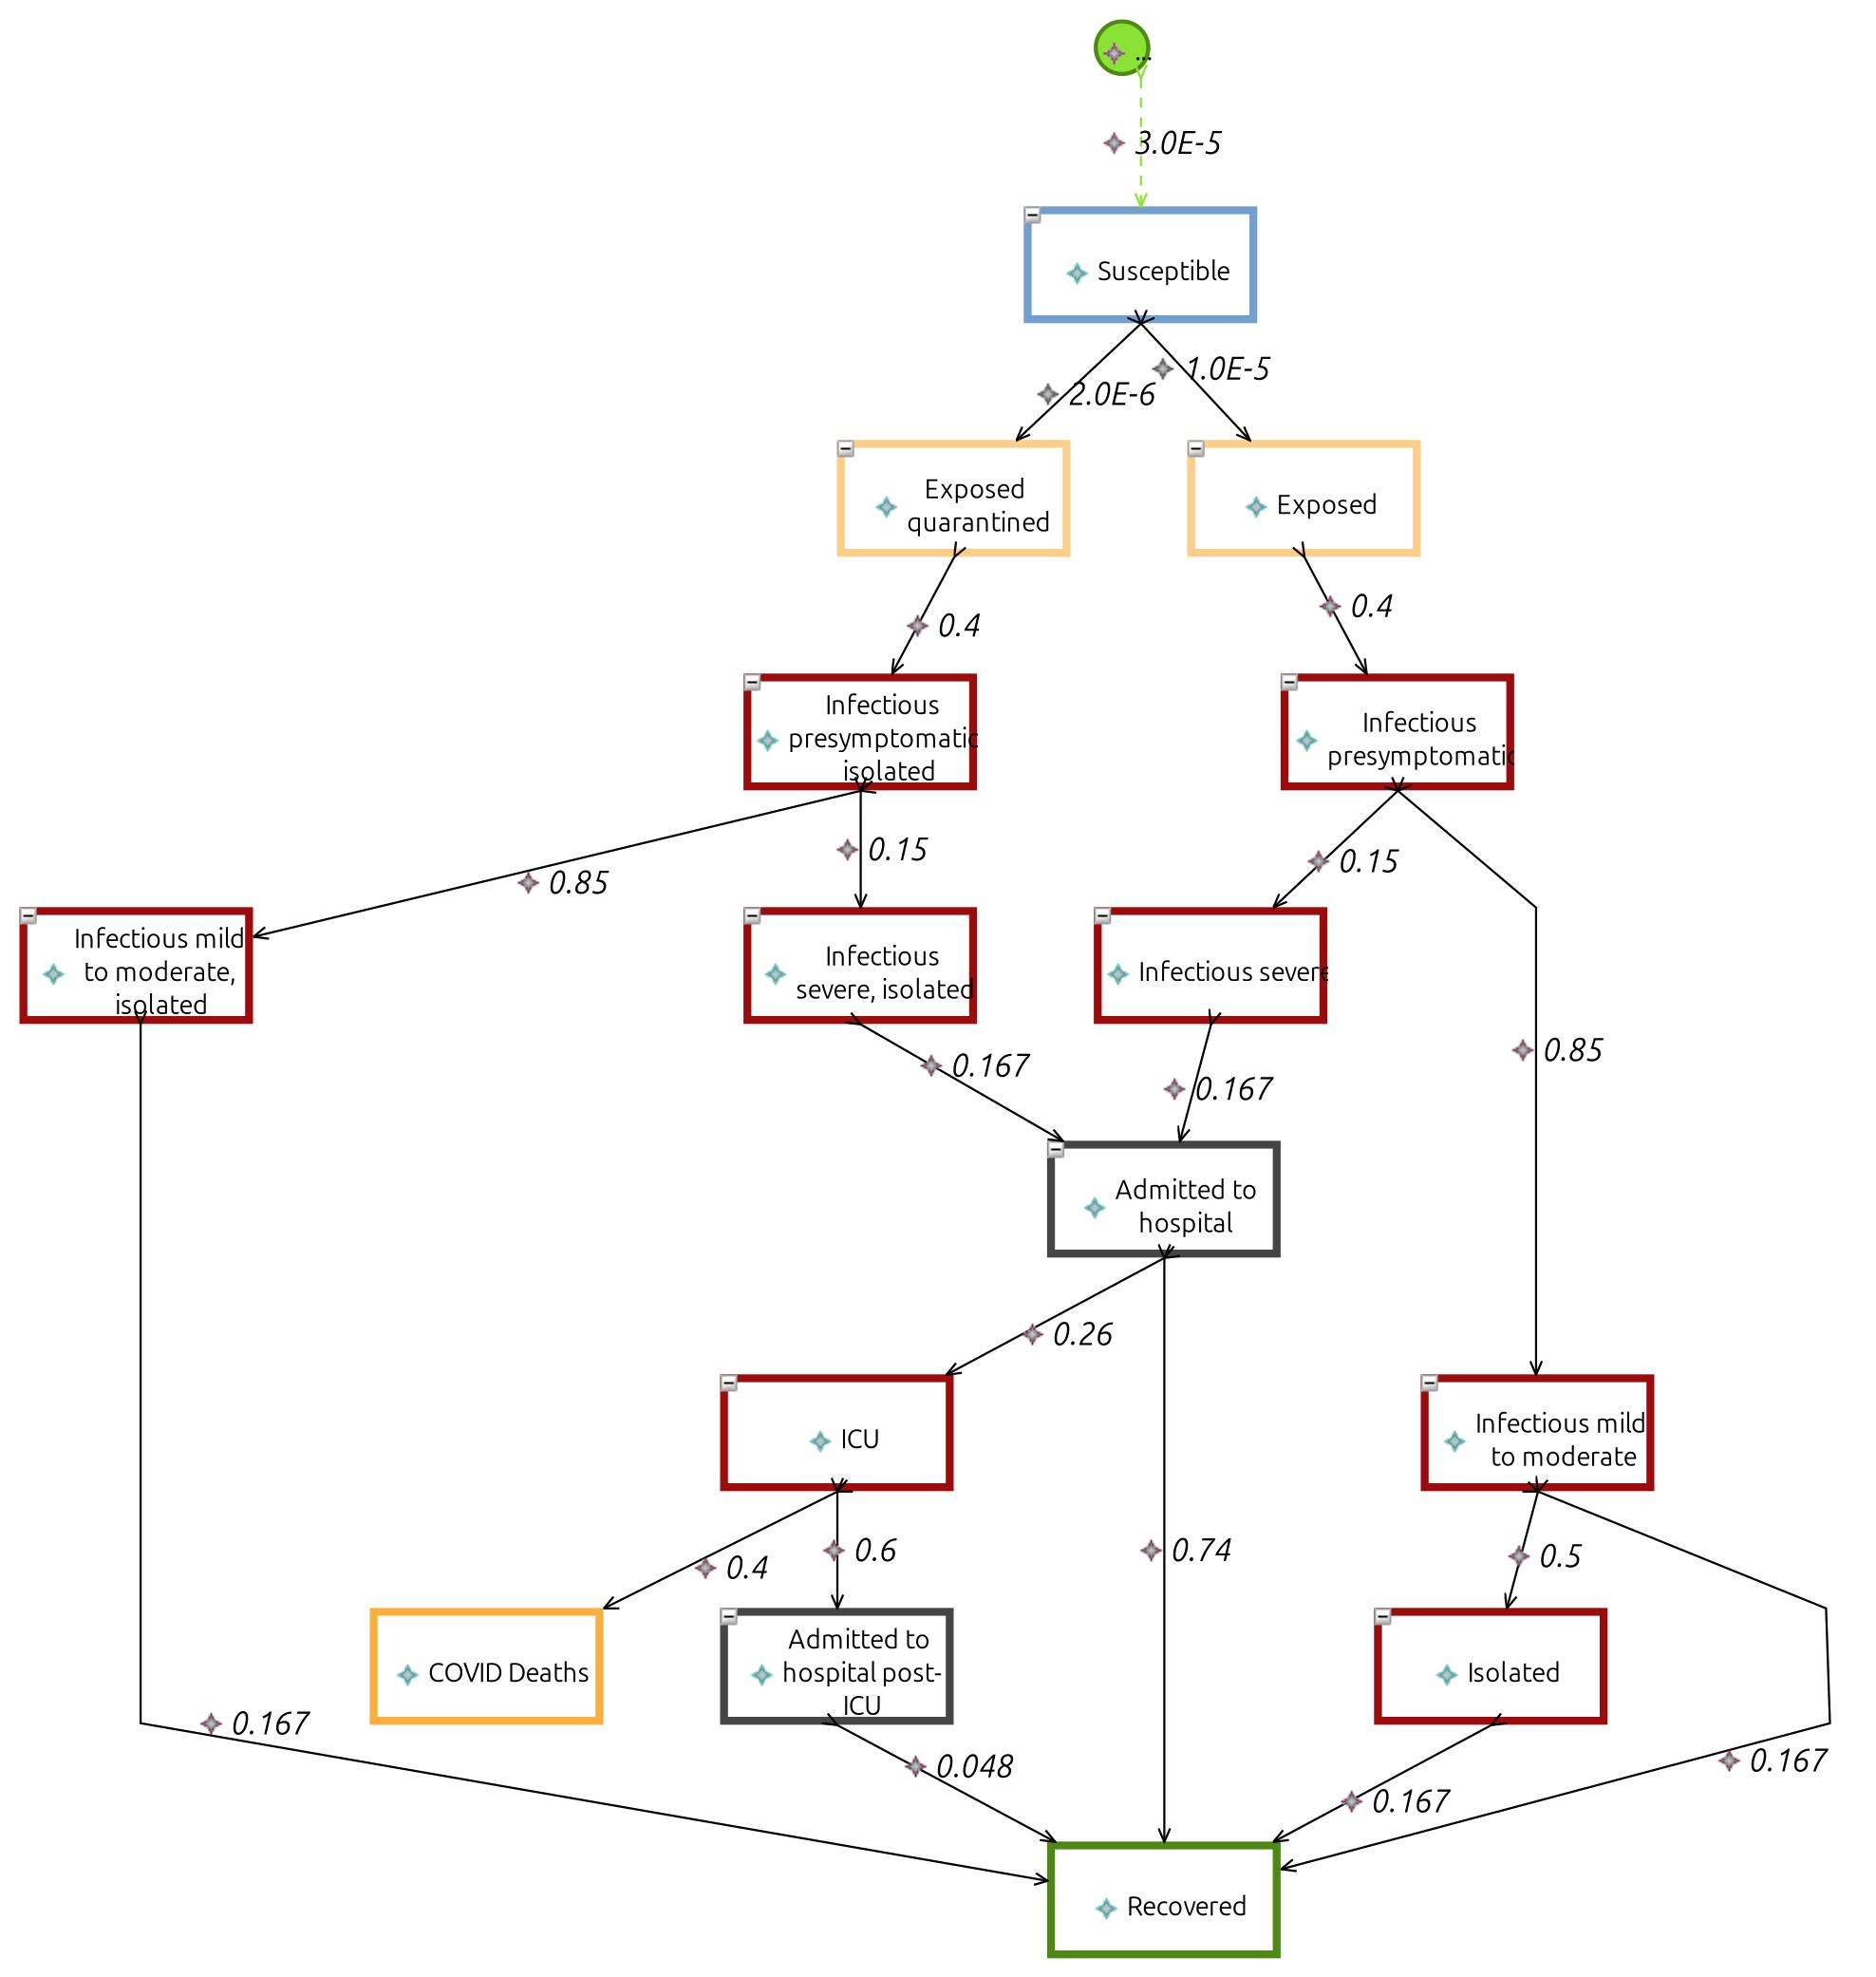
\includegraphics[width=0.8\textwidth]{Figures/Covid.jpg}
    \caption{Graphical representation of the COVID-19 SEIR model in EpiMDE Lite.}
    \label{fig:covid_model}
\end{figure}

While the basic modeling approach with EpiMDE is good for quickly replicating the original work, the resulting model suffers from the shortcomings of the original model, i.e., reduced replicability and verbosity, in terms of number of compartments and flows. In addition, certain parameters of the original model, such as age groups, could not be easily ported in the EpiMDE model. To this end, we also explored the capabilities of the extensible metamodel and we used groups and products, as well as complex flows, to better organize the model, through better modularity and separation of concerns, and facilitate more of its advance functionalities.

First, looking at the naming and coloring of the elements in the original diagram, we can see that orange refers to isolated, while purple refers to not isolated. Susceptible, exposed, hospitalized and recovered are also color coded. We begin by creating a group to place our elements into, then place unit compartments for S, R and Dead. E and I share commonalities, specifically, they are both stratified along isolation status. We will create a product to hold two groups: isolation and E-I. The isolation group simply has a isolated and non-isolated unit compartments. E-I has two groups, E and I, which have their purple and orange compartments from the original figure, so E is a compartment but I is a group containing presymptomatic, mild and severe.

%The researchers responsible for the studied model made the decision not to include "within-hospital transmission cycles"\cite{TuiteE497}. For this reason, we can leave hospitalization out of the infectious group as they will not be used as contacts for transmission. Hospitalization will be a group with units for no-icu, pre-icu, icu and post-icu. 
%Figure \ref{fig:tuite-cp1} shows the structure so far.

%\begin{figure}[H]
%    \centering
%    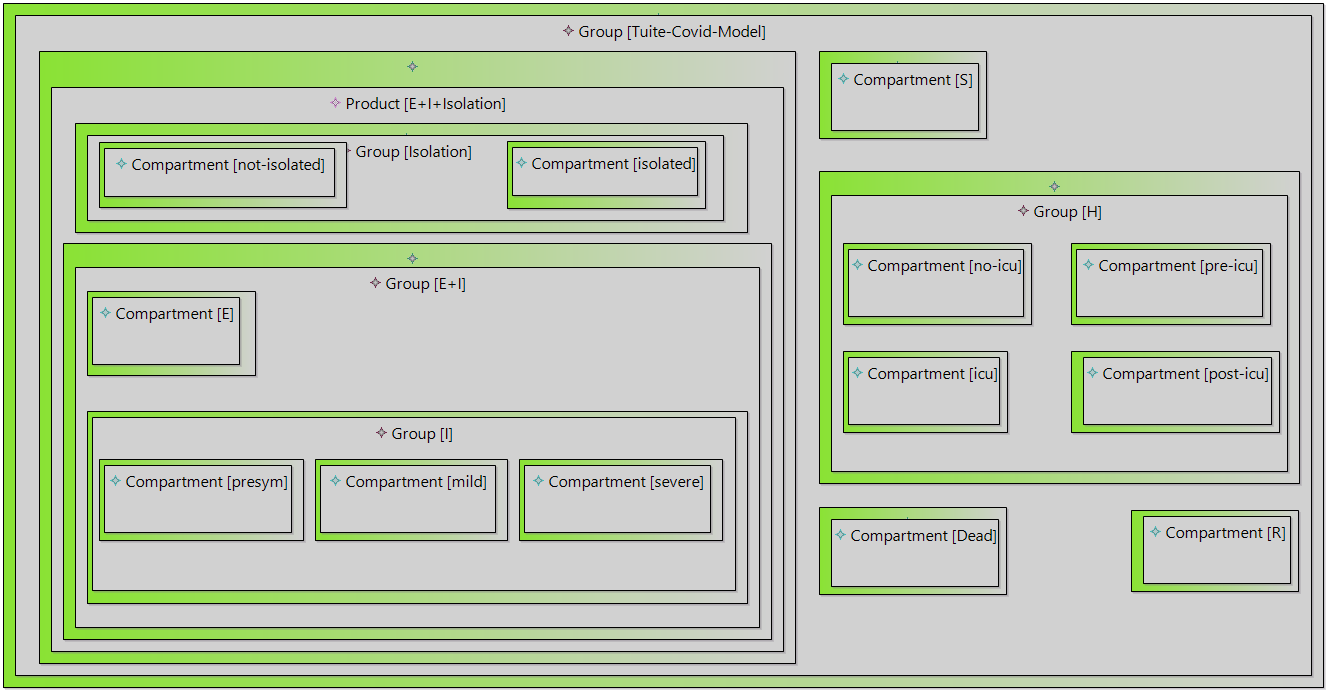
\includegraphics[width=\linewidth]{Figures/tuite-cp1.png}
%    \caption{Model Structure}
%    \label{fig:tuite-cp1}
%\end{figure}

After modeling the structural aspect of the model, it is time to model the behavioural aspect, by using flows. The original model contains 21 flows, but by using flows on composites, we can reduce this amount. As a model's size increases, applying flows to structures instead of individual components saves time and complexity. It also dissociates a composite's contents from the flows, allowing for inner structure modification without change to the flows. This is visually apparent in the resulting model, as shown in Figure \ref{fig:tuite-cp2}. There are now 11 flows instead of 21. Flows in our platform are named diamonds with named reference, which may help clarify the model. For example, the authors mention: "Testing was assumed to move individuals with nonsevere symptoms from the infectious to isolated compartments" \cite{TuiteE497}, while in our model we can simply name this flow "testing".

\begin{figure}[t]
    \centering
    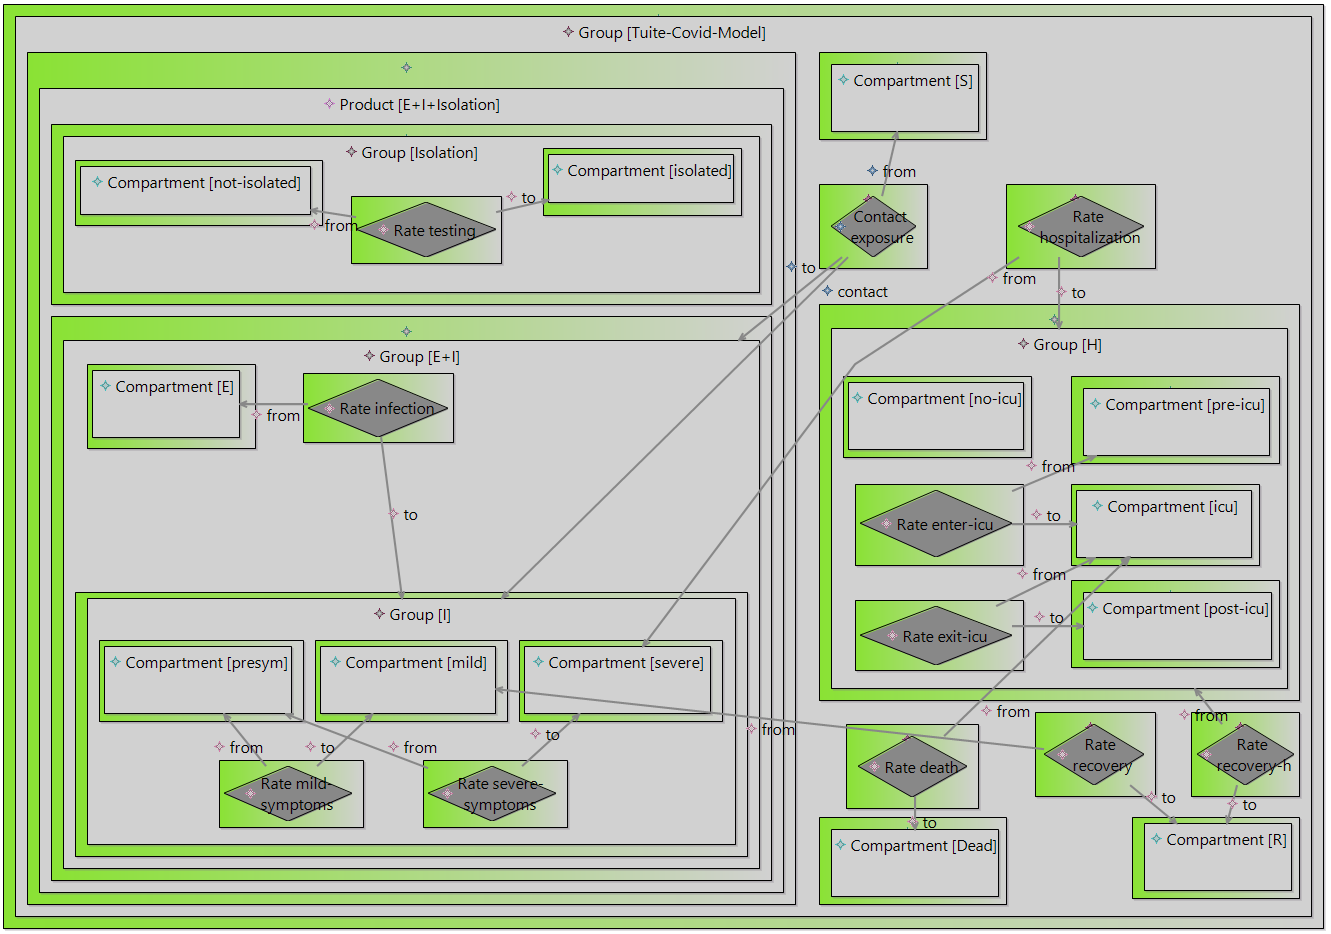
\includegraphics[width=\linewidth]{Figures/tuite-cp2.png}
    \caption{Model Structure and Flows}
    \label{fig:tuite-cp2}
\end{figure}


The final step is model stratification along age and comorbidity, which is simply done by placing the model in a product along with the age dimension and the comorbidity dimension. As seen in the original model, stratification along age and comorbidity is not represented graphically, which is not the case for EpiMDE. The result is a simple model of a product between age groups, which can be used in the larger model as a link (i.e., an expandable reference to an external model), and a comorbidity option.
%, as shown in Figure~\ref{fig:tuite-cp4}.

%\begin{figure}[H]
%    \centering
%    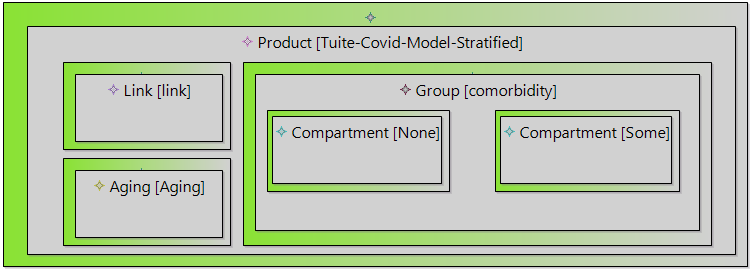
\includegraphics[width=\linewidth]{Figures/tuite-cp4.png}
%    \caption{Stratified Model}
%    \label{fig:tuite-cp4}
%\end{figure}

The Link and Aging compartments are simple metamodel extensions. Link allows us to reference compartments from other model, here we reference the top level element from the previous model. Aging allows us to provide a list of age groups as a string, in this case, for the Canadian health data, we provide ``0-4, 5-9, 10-14, 15-19, 20-24, 25-29, 30-34, 35-39, 40-44, 45-49, 50-54, 55-59, 60-64, 65-69, 70+", which generates compartments as well as rates between the consecutive age groups.

\subsubsection{Model validation}

Model validation involves comparing the expected output of a model with the actual output. The output may be thought of as the graph produced for an entire simulation, but, in practice, this may change based on simulation software. The derivative produced given a population distribution, however, is predictable.

In order to compare models, we randomly generated population distributions to compare both models' derivatives. The reference model's derivative is the expected derivative of the model being validated. In the event where the two are identical, the validation is done. In the event where the two are different, we need to refine the incorrect model and ideally identify where the differences come from. This is an aspect of the project which presents an opportunity for usability improvements.

For the context of this work, a validation script was produced which iterates over the names of our flows of this specific model and produces derivatives for both models based on an input. The original R code was transpiled to python and its equations were deconstructed in order to map the terms to names of equation. By writing a validation script which validates a projection of the model along a single equation, it is much easier to refine. Since flows in our platform are named and names are kept in the artifacts, we can easily toggle certain sets of equations by name. In the future, model validation may be further automated so that little to no programming may be involved for similar use cases, rendering this task simpler for epidemiologists.

\subsubsection{LLM-Based Automated Generation Results}

The COVID-19 model presented a more complex generation challenge than HIV, with 63 total elements including 15 compartments across multiple disease stages (exposed, infectious subtypes, hospitalization states), 23 parameters, age-based stratification, and 19 flows representing disease progression and intervention pathways. This model's larger element count and intricate flow network tested the LLM pipeline's scalability.

\begin{table}[htbp]
\centering
\caption{LLM Performance for COVID-19 Model Generation}
\label{tab:covid_llm_performance}
\begin{tabular}{lccc}
\hline
\textbf{LLM Model} & \textbf{Precision} & \textbf{Recall} & \textbf{F1 Score} \\
\hline
GPT-4o & 91.1\% & 65.1\% & 0.759 \\
Gemini 2.5 Pro & 100\% & 100\% & 1.000 \\
\hline
\end{tabular}
\end{table}

\textbf{GPT-4o Performance:} The pipeline achieved high precision (91.1\%) but significantly lower recall (65.1\%), yielding F1 = 0.759. While compartments, parameters, groups, and products were correctly generated, 22 of the 19 specified flows were either completely absent or generated with incorrect structure. The user input clearly listed all flow transitions, but these did not materialize in the final XML with proper \texttt{<outgoingFlows>} elements. This failure mode differs fundamentally from the HIV model's indexing errors and suggests two contributing factors: context window pressure from the substantially larger specification approaching GPT-4o's effective context limits, and potential prompt ambiguity in translating complex flow networks into XML. The 4 false positives represented attribute hallucination where the model generated \texttt{multiplier} attributes within \texttt{<stratumSpecificRates>} for age-dependent transmission rates—conceptually reasonable but not part of the metamodel specification. Despite XML generation challenges, the Stage 3 simulation script executed successfully using validated ODE equations, producing correct time-series plots for all age-stratified compartments.

\textbf{Gemini 2.5 Pro Performance:} In stark contrast to GPT-4o, Gemini achieved perfect generation with Precision = 100\%, Recall = 100\%, F1 = 1.000. All 63 elements were correctly generated with no hallucinations and no omissions. Critically, all 19 flows appeared with proper structure, correct \texttt{xsi:type} classification (RateFlow vs. ContactFlow), accurate \texttt{target} references, and appropriate parameter linkages. The flow omission pattern that plagued GPT-4o did not occur, suggesting the failure was not inherent to task complexity but specific to GPT-4o's context management or instruction-following capabilities for this prompt structure. The simulation script generation succeeded with compact, semantically organized code that logically grouped compartments and improved human readability while maintaining 100\% execution correctness.

\textbf{Key Findings:} The dramatic performance divergence between GPT-4o and Gemini reveals that COVID-19 model generation is a context-intensive task requiring state-of-the-art LLM capabilities. GPT-4o's systematic flow omissions indicate it reached capacity limits handling the specification's size and complexity, while Gemini's perfect generation demonstrates that frontier models possess sufficient capacity for complex epidemiological models. This has practical implications: as models grow in complexity (more compartments, deeper stratification, intricate interventions), access to cutting-edge LLMs transitions from optional to necessary. The perfect simulation generation by both models (despite XML differences) again validates the robustness of the two-phase skeleton approach, which successfully isolated Stage 3 from Stage 1-2 errors by operating on independently validated ODE equations.



\subsection{Case Study 3: Illustrating Support for Rapid Prototyping}
\label{sec:casestudy:prototyping}
% \subsection{Introduction and Motiv<ating Example}
% \label{subsec:carol-example-introduction}


EpiMDE is designed to support workflow extensions implemented as separate layers on top of the core platform. It exposes the metamodel and model repository through an EMF based API, enabling external analyses (e.g., clustering, differencing, logical consistency checks) to be integrated without modifying the platform itself. In our third case study, we examine how well EpiMDE supports epidemiological workflows, by developing an illustrative example. 
Specifically, we use a rapid prototyping scenario~\cite{fiyouzisabah2024towards} to probe whether the platform provides sufficient expressiveness and extensibility to support the construction of workflow-specific tooling on top of EpiMDE.
% Specifically, we probed how well the platform can be used to build a tool for rapid prototyping of epidemiological models, in a context that arises when a new disease is discovered. 
We studied the research question: 
\textit{What challenges and opportunities arise when applying a purpose-built modeling infrastructure to the development of domain-specific modeling workflows?} 
The lessons learned reveal both the platform’s strengths and its friction points.

We assume a persona named ``Carol'' working under the pressure of a health crisis (like the COVID-19 pandemic) to quickly create and validate an epidemiological model. 
Carol hopes to rapidly prototype a new model by reusing previously developed, tested, and validated model components to accelerate her work. 
So, she wants to identify and select useful modeling elements and assemble them into a partially completed prototype, avoiding redundant re‐implementation efforts. 
She hopes that, using this prototype model as a base, she can focus on her study's unique aspects and design and integrate new features. 
All models and generated artifacts from our scenario are included in our replication package published on Zenodo~\cite{zenodo_17806440}.

We assume that Carol starts with a corpus made up of the three previously developed compartmental models shown in Figure~\ref{fig:prototype_submodels}. 
Each one contains elements that may be relevant and useful for her own study. 
For instance, the model $m_1$ in Figure~\ref{fig:prototype_m1} includes exposed and vaccinated groups.
The model $m_2$ in Figure~\ref{fig:prototype_m2} adds more details about disease spread by breaking down the infectious population into asymptomatic, mildly symptomatic, and severely symptomatic compartments. 
Finally, the model $m_3$ in Figure~\ref{fig:prototype_m3} contains the hospitalization status of individuals, allowing to better model the load to the healthcare system.
Typically, Carol would have to manually search through the corpus of existing models, identify which parts are relevant, extract them, and then integrate them into her own model.
This is time-consuming and error-prone. 
Using the EpiMDE platform, we can simplify this process by creating an interactive layer that guides users like Carol through the steps for reusing previous work. 
Carol only needs to provide a repository of existing models. 
The tool then follows the workflow explained later (see Subsection~\ref{sec:prototyping_workflow}) to analyze these models and identify potentially relevant components. 
Finally, Carol can select the parts she wants to reuse, and the tool will automatically generate a prototype model that includes the selected items. 
She can then use this as a partially completed prototype on which to base the rest of her modeling efforts. 

\begin{figure}[t]
\centering
\begin{subfigure}[b]{0.40\textwidth}
  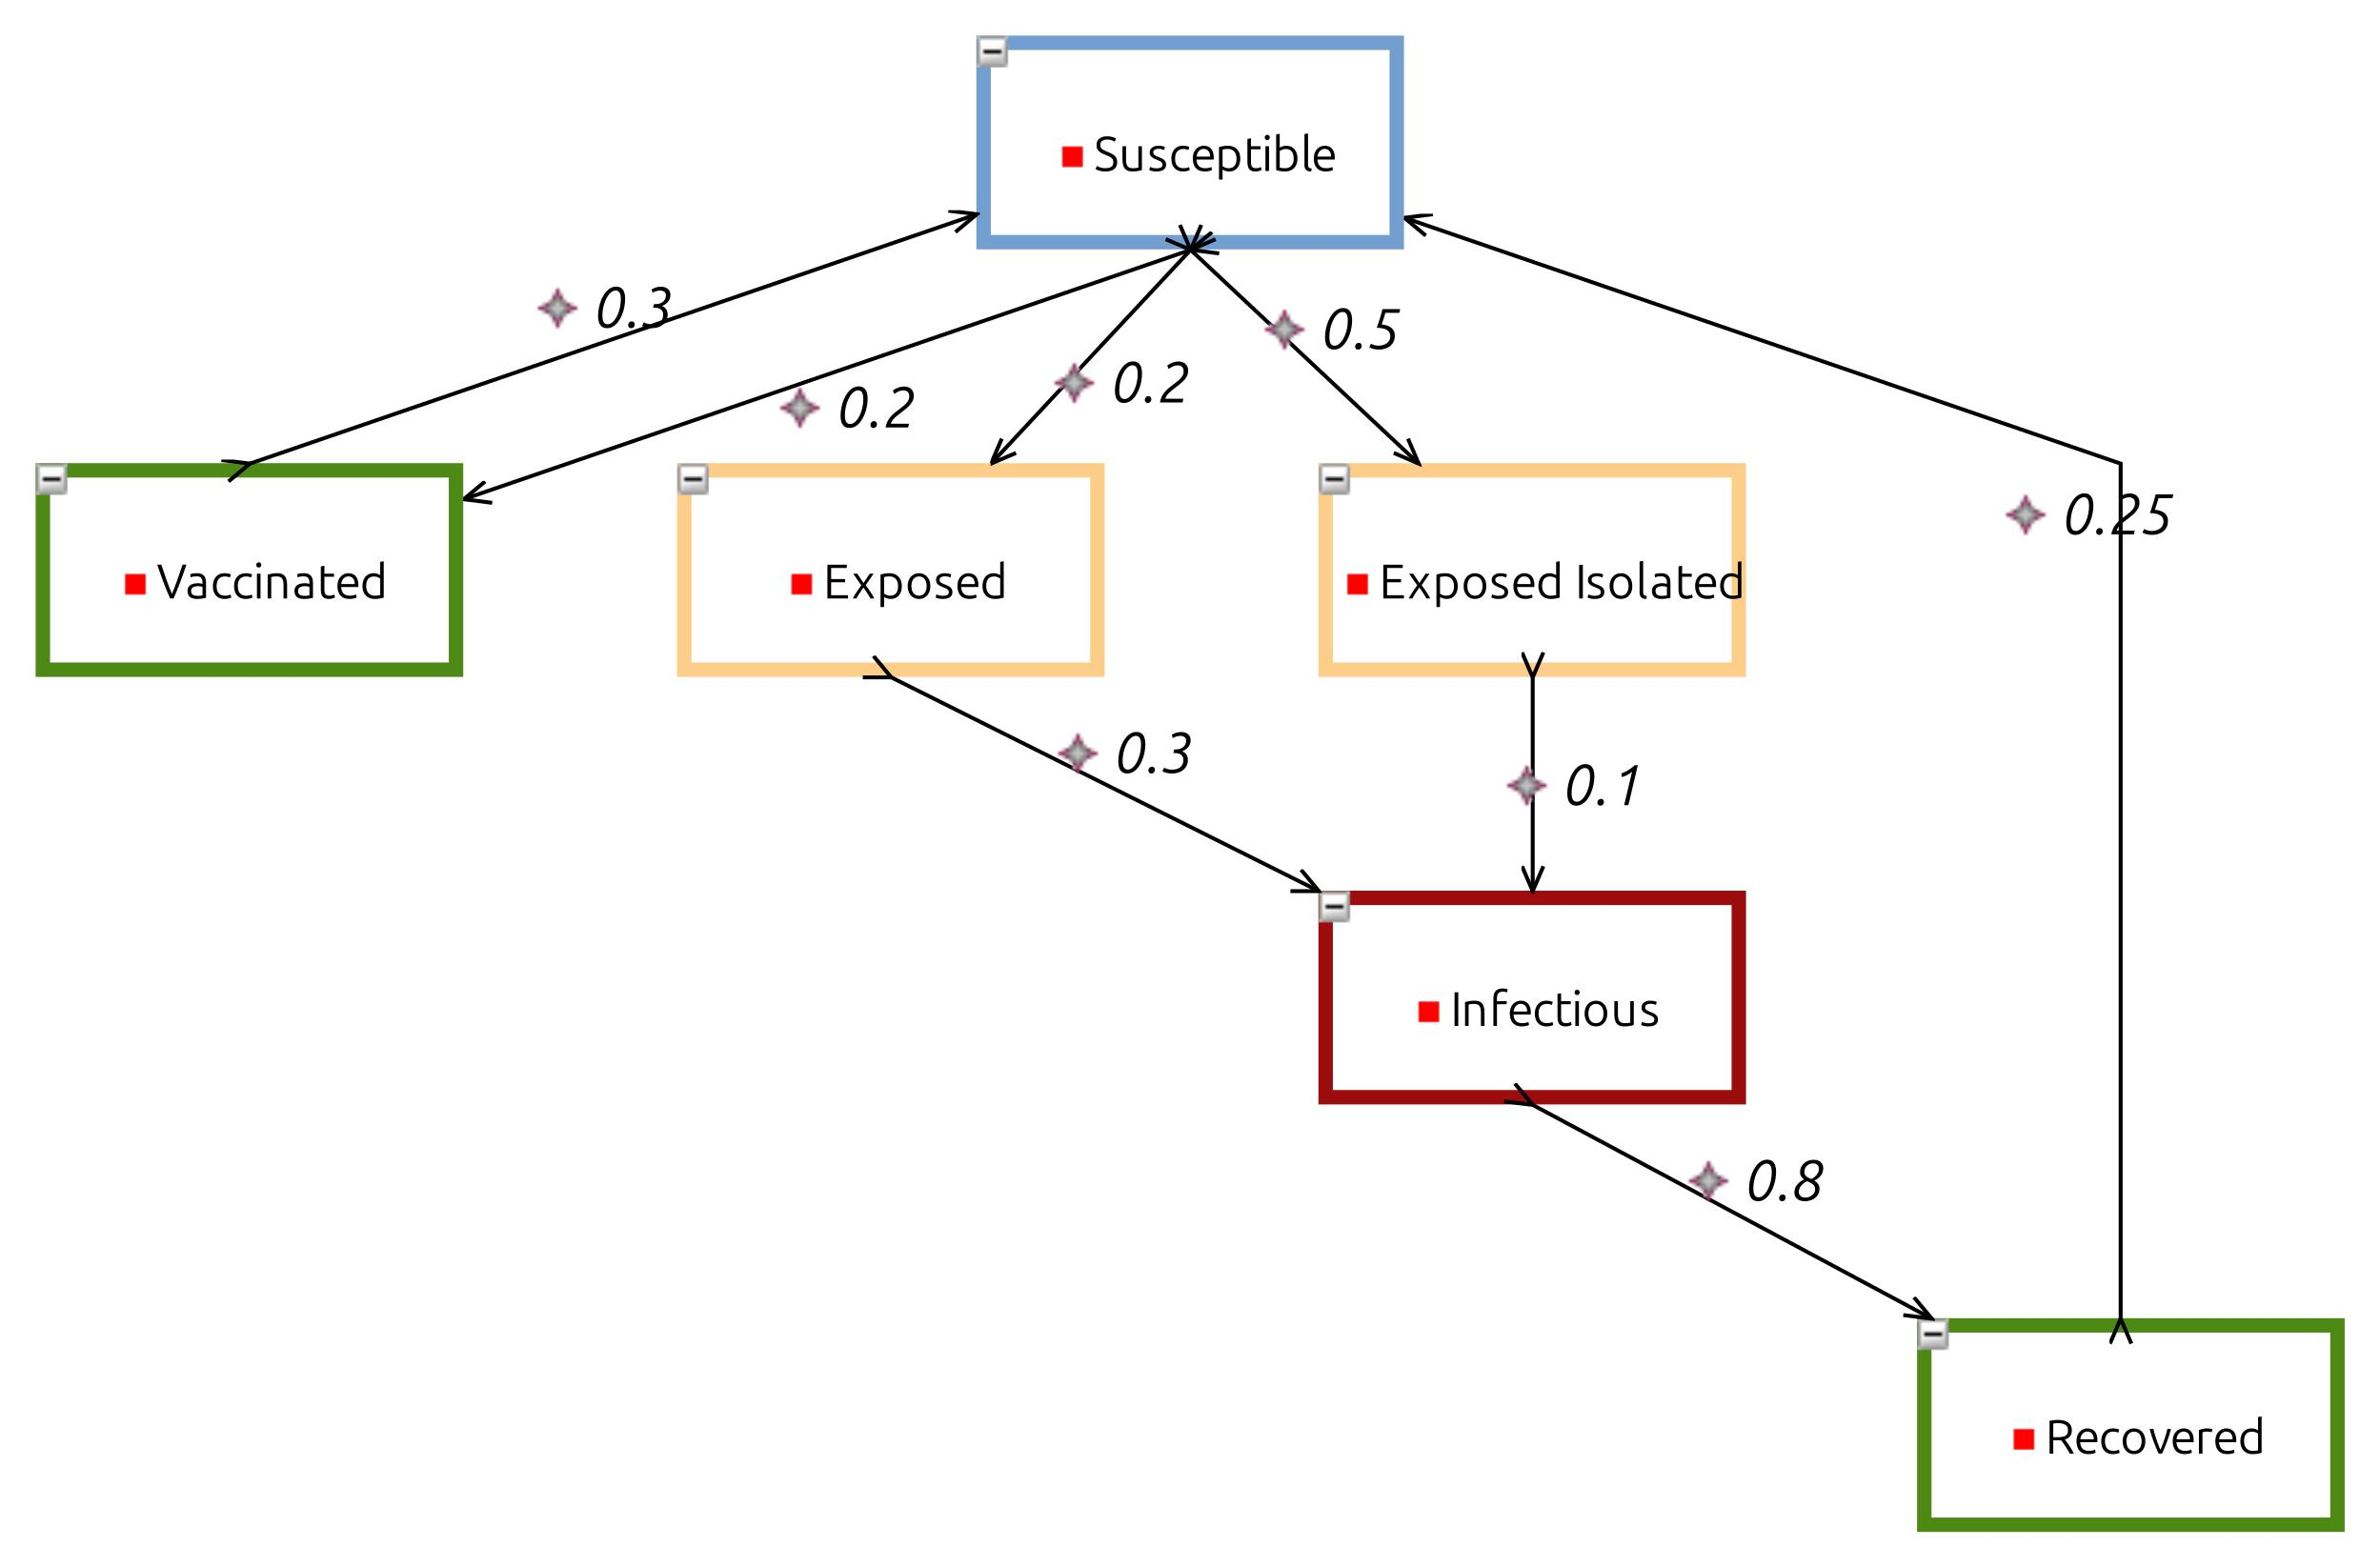
\includegraphics[width=\textwidth]{Figures/paper1.jpg}
  \caption{$m_1$}
  \label{fig:prototype_m1}
\end{subfigure}
\begin{subfigure}[b]{0.40\textwidth}
  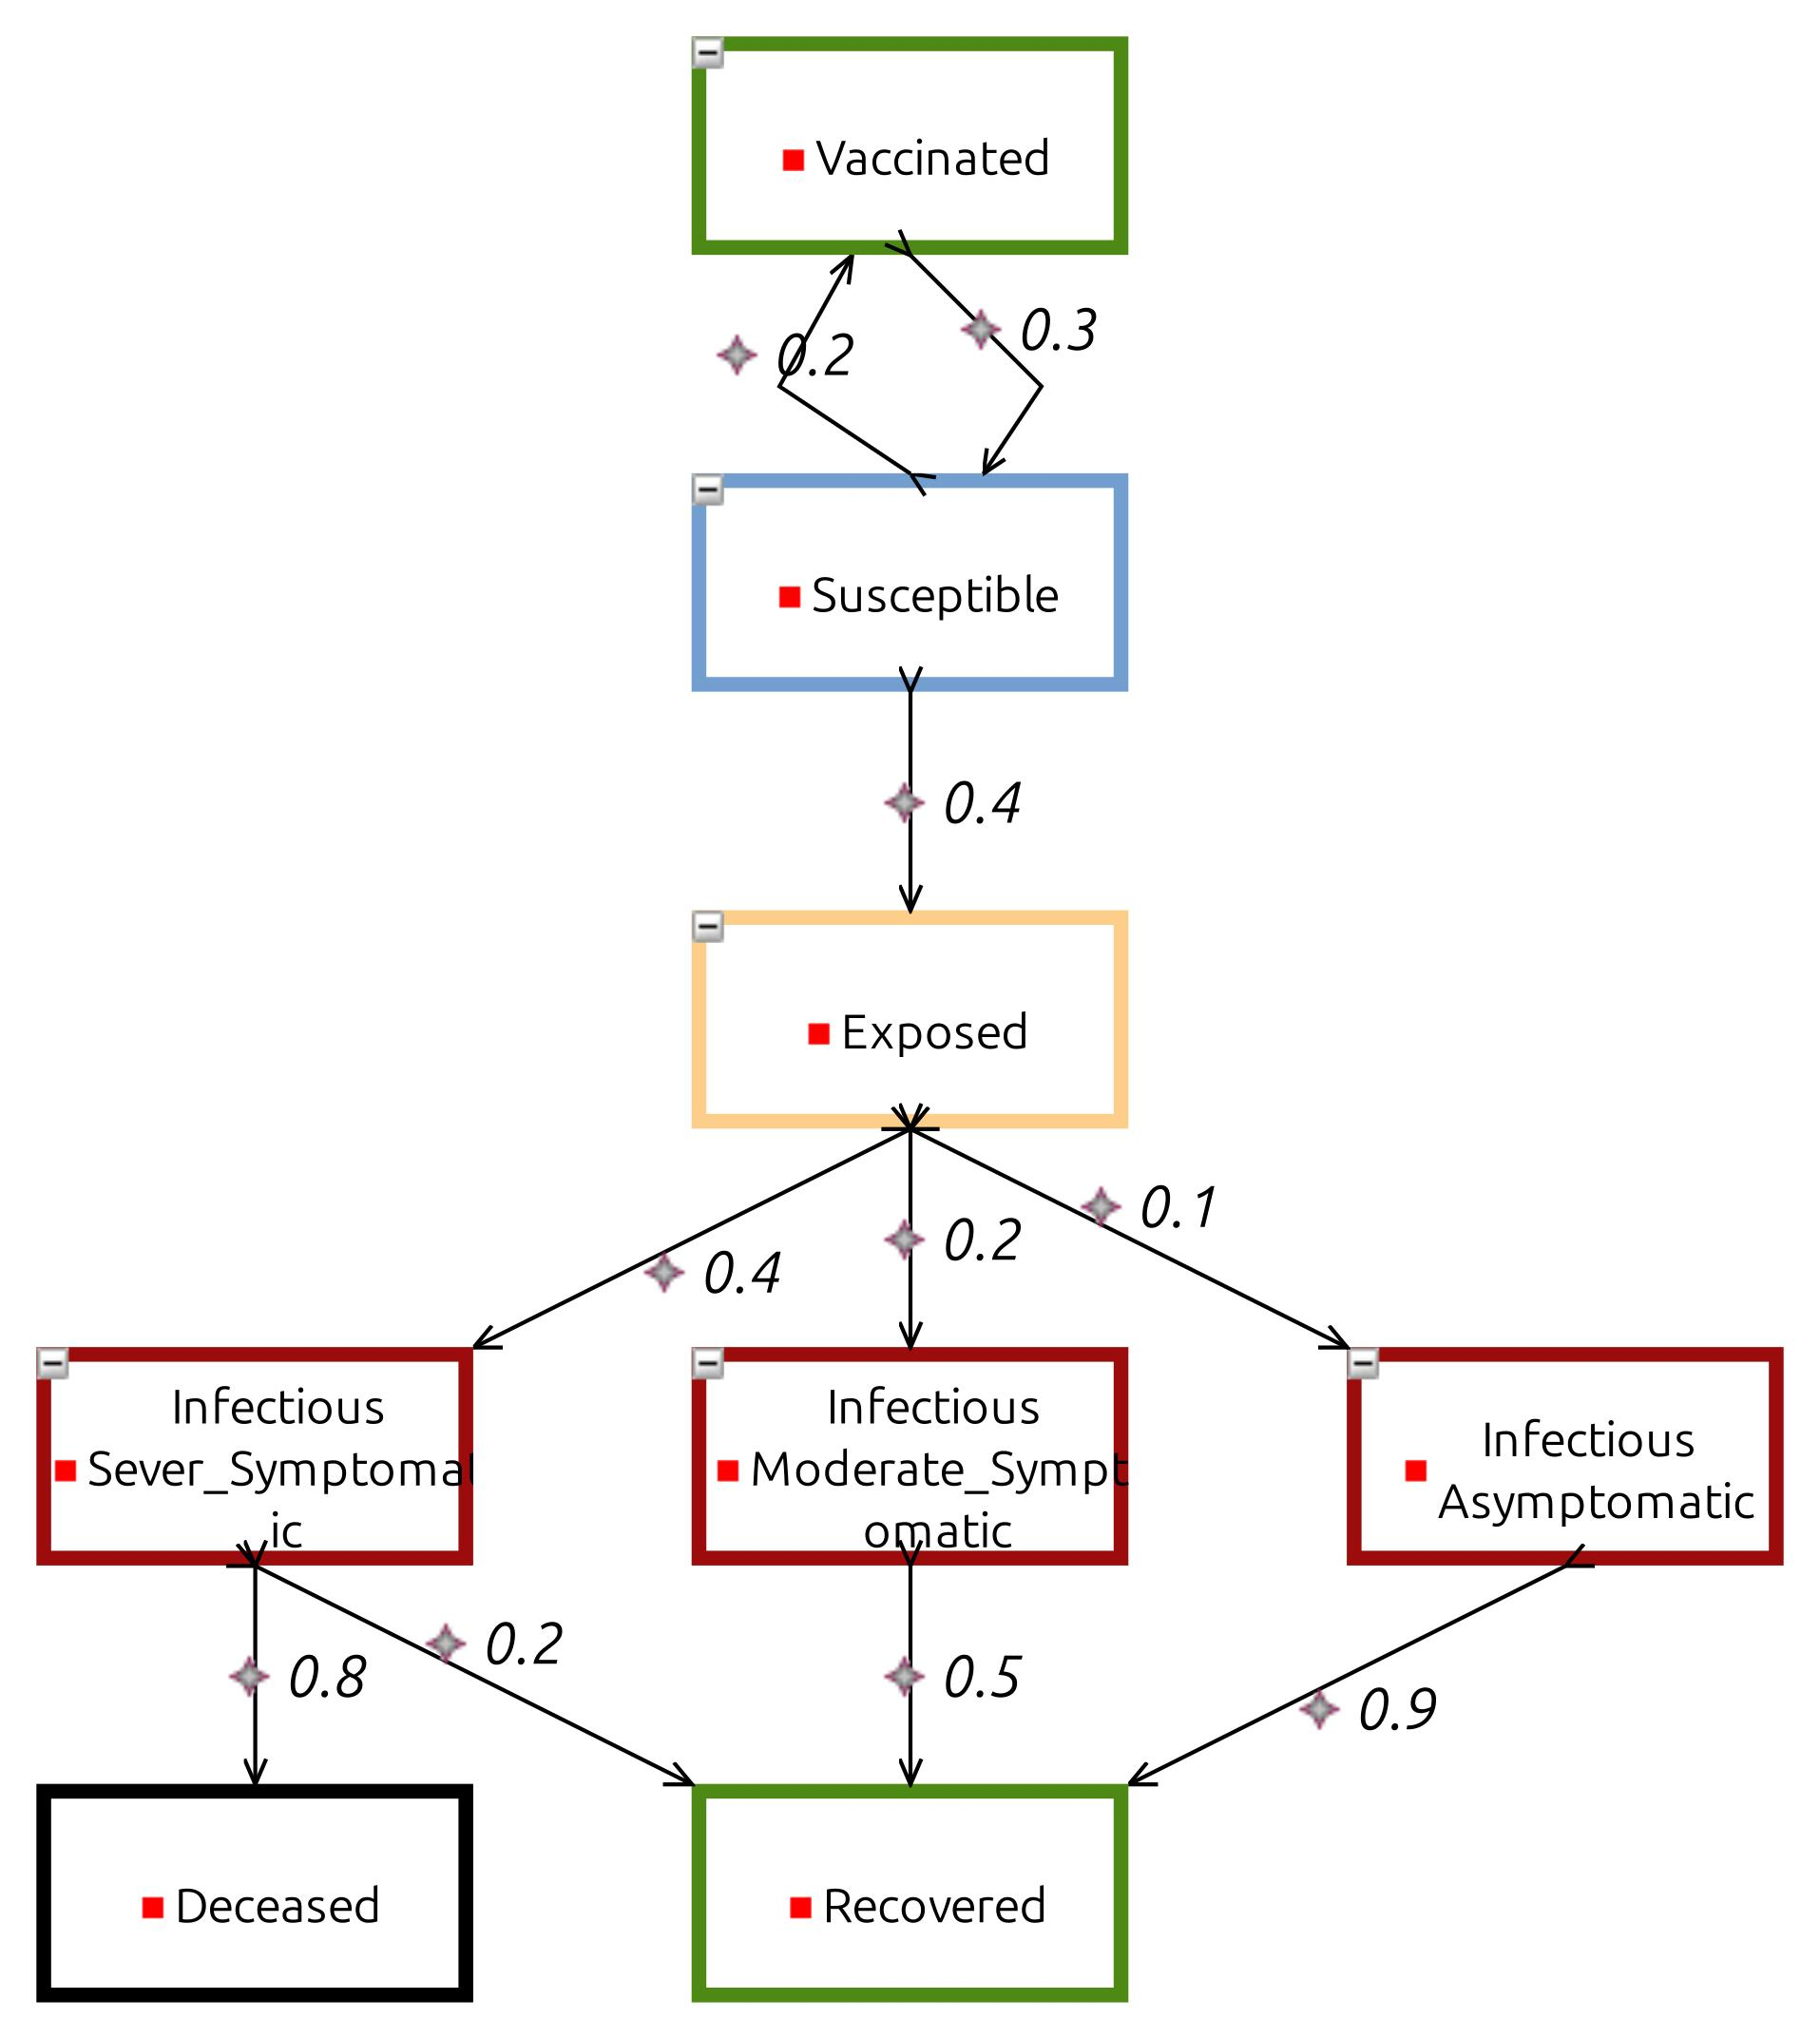
\includegraphics[width=\textwidth]{Figures/paper2.jpg}
  \caption{$m_2$}
  \label{fig:prototype_m2}
\end{subfigure}
\begin{subfigure}[b]{0.40\textwidth}
  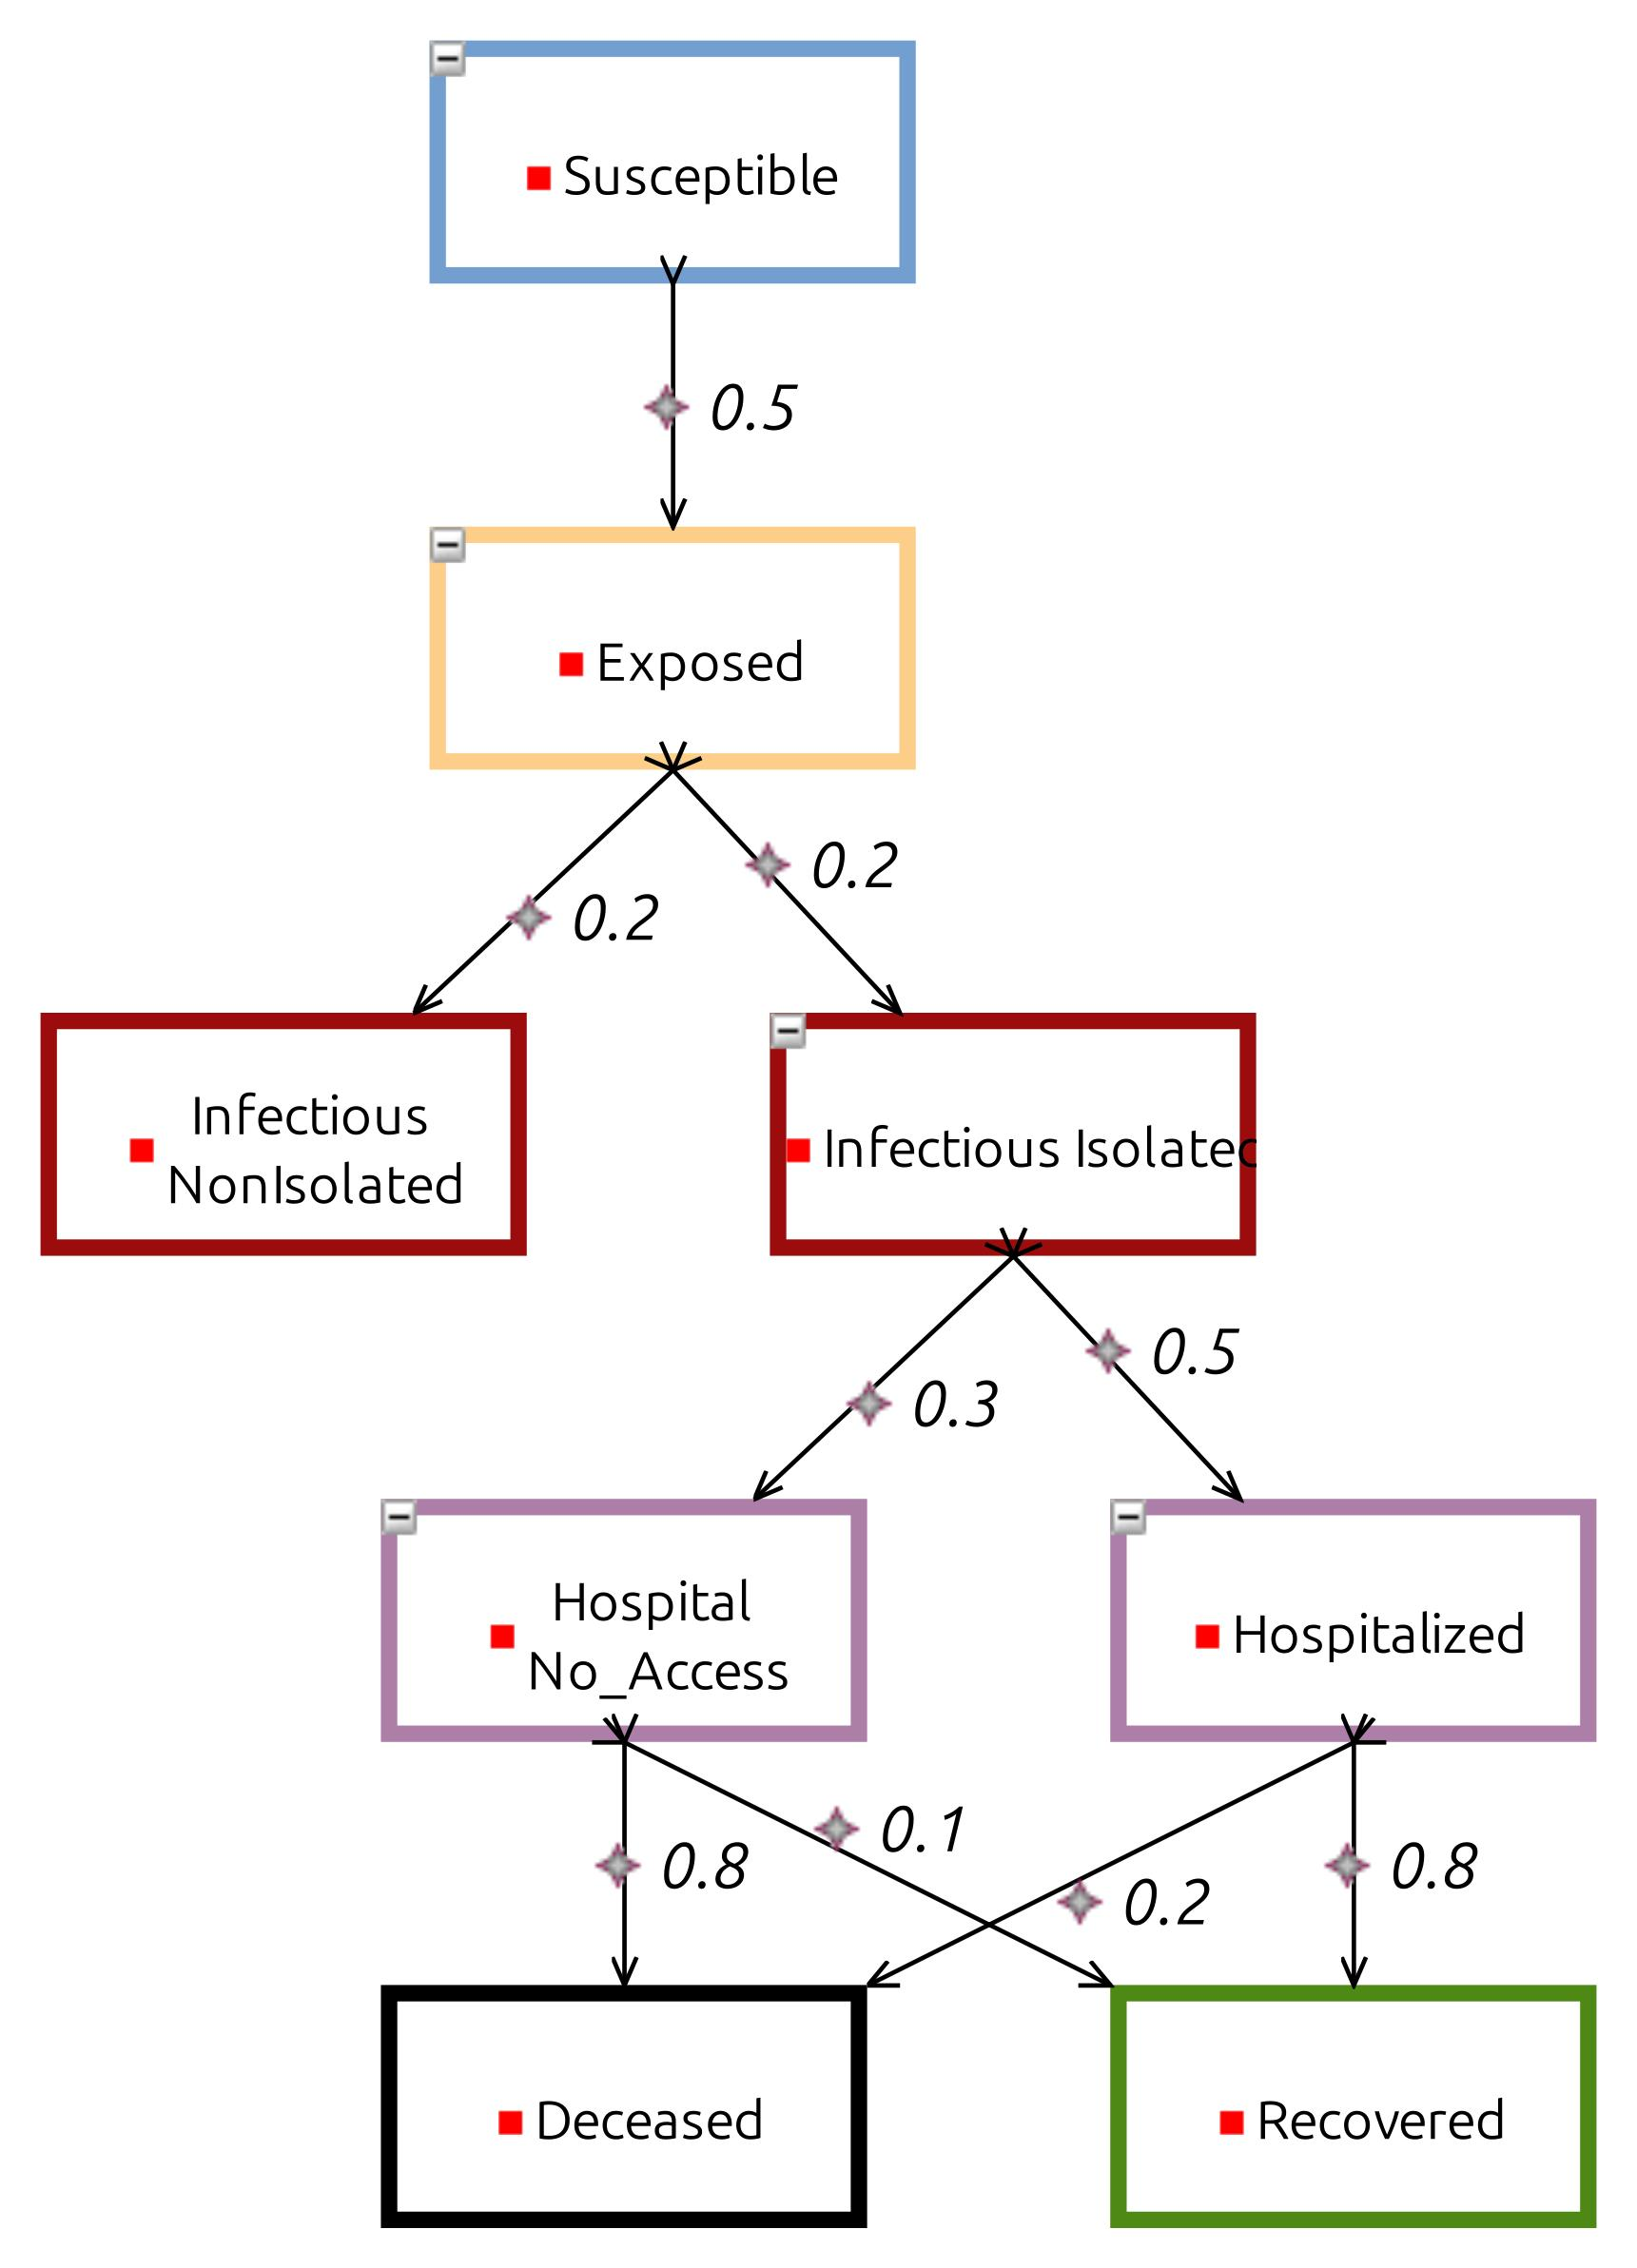
\includegraphics[width=\textwidth]{Figures/paper3.jpg}
  \caption{$m_3$}
  \label{fig:prototype_m3}
\end{subfigure}
\caption{Corpus of prior compartmental models to consult.
}
\label{fig:prototype_submodels}
\end{figure}

% \subsection{Approach}
%to help epidemiologists seamlessly reuse modeling ideas from previous models and rapidly integrate them into a prototype model, which they can use for further development. Below, we explain the four steps of our approach.

\subsubsection{Workflow}
\label{sec:prototyping_workflow}

We implemented the workflow as an external layer on top of EpiMDE. It operationalizes a prototyping-specific notion of ``relevance'' to support rapid model construction under time pressure. EpiMDE itself does not prescribe a canonical relevance metric or workflow; rather, it provides the model representations, APIs, and analysis hooks required to implement such workflows.

Concretely, the workflow layer leverages programmatic access to EpiMDE models and metamodel instances, stable element identifiers, and integration with third-party analysis tools. The heuristics used to identify and rank potentially relevant components are intentionally workflow-specific, and are presented here to demonstrate that EpiMDE provides sufficient expressive power and extensibility to support domain-specific modeling workflows.

We build the interactive rapid prototyping EpiMDE layer in four steps.

\paragraph{Variation Point Extraction:} 
First, we identify commonalities and differences in the input corpus.
For example, the compartment \textit{Susceptible} appears in all models ($m_1$-$m_3$), so we consider it a commonality indicating the same epidemiological concept. 
On the other hand, the compartment labeled \textit{Hospitalized} only appears in $m_3$: the other models do not concern themselves with this concept.

Note that although the models in the corpus may describe different diseases, identifying variation points remains meaningful. Many epidemiological concepts, such as the \textit{Susceptible} compartment, represent fundamental population states rather than disease-specific mechanisms. Thus, commonalities can still capture shared modeling structures that are valuable for constructing new prototypes even when the models target distinct pathogens. Of course, if the input corpus contains models of the same disease, the identified variation points are likely to be more disease-specific and semantically aligned.

To systematically identify \textit{variation points}, we assign unique identifiers (IDs) to the model elements, as follows: 
%A variation point represents a model element in a way that allows us to determine whether it is shared across models or distinct. The IDs are defined as follows:
%\begin{itemize}
    %\item 
(a) For compartments, the ID is simply the name of the compartment.
    %\item 
(b) For rates, flows, etc., the ID is a combination of the source compartment ID, target compartment ID, and the flow rate expression.
%\end{itemize}
%
When two elements share the same IDs, they are considered the same, but if their IDs are different, they are treated as variants. 
%This step helps identify common parts shared among models, laying the groundwork for extracting meaningful \textit{features} in the next steps.

% In the first step, our tool extracts the variation points from the existing models that Carol intends to reuse.
In Carol's case, for example
%an ID to each model element to identify which variation points are shared or unique across models. For compartments, we use the compartment name as the Variation Point ID. For example,
in model $m_1$, EpiMDE creates IDs for compartments such as \textit{Susceptible} and \textit{Vaccinated} %, and \textit{Exposed}.% are treated as distinct variation points. 
and IDs for flows such as %the ID is constructed by combining the source and target compartments as well as the flow rate. For instance, 
$Susceptible\_Vaccinated\_0.2$. 
%refers to a flow from \textit{Susceptible} to \textit{Vaccinated} with a rate of 0.2. 
% Using these IDs allows the tool to consistently detect and assign variation points to models. 
We show the complete list of variation points assigned to the models $m_1$, $m_2$, and $m_3$ in the Appendix Table~\ref{tab:prototype_variation_points}.


\paragraph{Feature Identification:} 
Next, we identify collections of variation points that appear together in the corpus and cluster them accordingly. 
These clusters likely represent features~\cite{berger2015feature}, pending confirmation by the epidemiologist.
We use Formal Concept Analysis (FCA), a mathematical framework used in data analysis and knowledge representation~\cite{ganter2012formal}
to classify objects based on shared attributes. 
Specifically, we integrated EpiMDE with FCA4J library~\cite{gutierrez2022fca4j}, 
which allows us to identify recurring patterns based on their shared variation points.%, identified by their unique IDs. 
%This allows us to detect shared variation points across different models, 
%that appear as recurring patterns that may represent modeling ideas or specific concepts that can be meaningfully reused together. 
%We then cluster these variation points to
We can thus identify potentially reusable components derived from existing models.
%
EpiMDE does this interactively, allowing Carol to change the automatically identified clusters.
This gives the epidemiologist the flexibility to split or reorganize clusters in case the mechanical clustering missed some relevant semantic nuance.
%This flexibility is important as some clusters might contain elements that are not related to each other, or the epidemiologist may prefer to reorganize them based on the specific needs of their study. 
We further prompt the epidemiologist to assign a meaningful label to each cluster. 
%These labels will make it easier for them to refer to and recognize the clusters further in the process. 
Once finalized and labeled, the refined clusters are henceforth referred to as \textit{features}. 


For Carol's three models
%In the second step, we apply Formal Concept Analysis (FCA) to the three models and their associated variation point IDs. 
FCA detects maximal groups of models that share a maximal set of variation points. 
We then cluster each of the identified sets of shared variation points to show the potential building blocks of existing models. 
For example, FCA identifies that all models share $Susceptible$, $Exposed$, and $Recovered$, which we put in the same cluster. 
% This set is identified by FCA, and we put them into the same cluster. 
This suggests that they often appear together and may represent a commonly reused pattern. 
Another example is the cluster formed by $Vaccinated$, $Susceptible\_Vaccinated\_0.2$, and $Vaccinated\_Susceptible\_0.3$, shared between $m_1$ and $m_2$. 
The fact that these co-occur in more than one place, indicates they might represent a common modeling idea that Carol would want to reuse together.

As a result of this step, EpiMDE generates the Appendix Table~\ref{tab:prototype_clusters}, which presents the clustered variation points. 
The table also includes a \textit{ClusterLabel} column initially left blank, allowing Carol to assign meaningful labels to each cluster. 
Carol can also refine and adapt the clusters as needed. 
We assume that she assigns the labels shown in the \textit{ClusterLabel} column and leaves the automatically identified clusters unchanged. 
Based on Carol's decision, each row in Table~\ref{tab:prototype_clusters} is considered to contain one \textit{feature}. 



\paragraph{Feature Relationship Identification:} Next, we identify relationships between features, such as dependency or mutual exclusivity. 
We always identify two relationships by default: 
%\begin{itemize}
    %\item 
(a)    A feature that contains a flow is always dependent on any other feature(s) containing the flow's source and target compartments. This ensures that compartments are well formed graphs.
    %This ensures that if we want to include the former in the prototype model, we also include the latter.
    %\item 
(b)    We assume that only one flow can exist between two compartments\footnote{Since compartmental models visualize differential equations, multiple arrows between the same compartments are redundant: they can be collapsed into a single arrow labeled with the sum of the rates. For our purposes, where the goal is to identify variation points between models, we treat differing rates as mutually exclusive alternatives, rather than cumulative effects.}. Thus if a feature contains a flow between two Compartments $A$ and $B$, it is mutually exclusive to  features that include other flows between $A$ and $B$.
%\end{itemize}
EpiMDE also prompts the epidemiologist to refine, customize and extend the set of identified feature relationships.
The resulting set of relationships are encoded in propositional logic, using the LogicNG library~\cite{logicng}.

In Carol's case, 
%In the next step, considering the features and the variation points each one contains, we identify the logical dependencies between features.
EpiMDE by default identifies the relatioship $Vaccination \Rightarrow Core\_SER$. 
This is because the $Vaccination$ feature includes a flow from \textit{Susceptible} to \textit{Vaccinated}. 
This flow relies on the existence of the $Susceptible$ compartment, which is part of the $Core\_SER$ feature, so $Vaccination$ depends on $Core\_SER$. 

Carol's case also includes mutual exclusivity relationships between features, such as the relationship
$Symptom\_Severity \Rightarrow \neg{Isolated\_Hospital} \land \neg{Exposed\_Isolation\_States}$. 
This is because $Symptom\_Severity$ has a flow from \textit{Susceptible} to \textit{Exposed} with a rate of 0.4, 
while $Isolated\_Hospital$ and $Exposed\_Isolation\_States$ also have flows between the same two compartments but with different rates. 
Based on our assumption that a compartmental model does not contain multiple flows between the same source and target compartments, 
EpiMDE identifies these features as mutually exclusive. 
The full set of the identified logical dependencies between features in Carol's example is available in the Zenodo replication package~\cite{zenodo_17806440}. 
In EpiMDE, Carol can further review, edit, or add to these constraints as needed. 




\paragraph{Feature Selection and Prototype Generation:} %With the features and necessary logical relationships between them at hand, it is time to construct the prototype model. 
To construct the prototype, Carol is prompted to select which combination of features she wants to include in her prototype.
%We ask the epidemiologist to select the features to include in their prototype model. 
%Providing a labeled list of features, using the labels that the epidemiologist assigned, makes it much easier for them to recognize and choose the relevant features that they want to include based on their specific modeling goals.
The epidemiologist can do this using the feature labels defined in Step 2.
%
To ensure her selection is valid with respect to the dependencies identified in Step 3, 
EpiMDE conjuncts all relevant relationship formulas and makes a satisfiability check using LogicNG. 
%the validity of user selection, we check its satisfiability according to the defined dependency rules, using an SAT solver along with the previously constructed LogicNG logical formulas. 
If the result is UNSAT, the epidemiologist is given a warning and asked to adapt her feature selection.
%If the solver finds the selection unsatisfiable, it means the combination of selected features does not work together logically. 
With a valid feature selection, we generate a prototype compartmental model that includes the appropriate features.
We implemented the feature merging in Java using the EpiMDE metamodel.

In Carol's case, EpiMDE prompts her to select from the list of features to include in the prototype model. 
We suppose that she selects $Mortality$ and $Exposed\_Isolation\_States$. 
EpiMDE checks for the satisfiability of the logical dependencies of her selection. 
They are satisfiable, and EpiMDE generates the model shown in Figure~\ref{fig:prototype_result_model}. 
In addition to Carol's selected features, the prototype model contains the feature $Core\_SER$, which Carol did not directly choose, but it is required based on the logical relationships between features. 
Carol can then treat this generated model as a prototype that reuses features from previous models.
She can then use it as the basis to develop a complete model according to her needs, without having to re-implement these features.
%completed, meaning that while it contains the desired features from existing work, Carol can evolve it further and add novel aspects specific to her study. 

% \end{enumerate}

 
\begin{figure}[t]
  \centering
  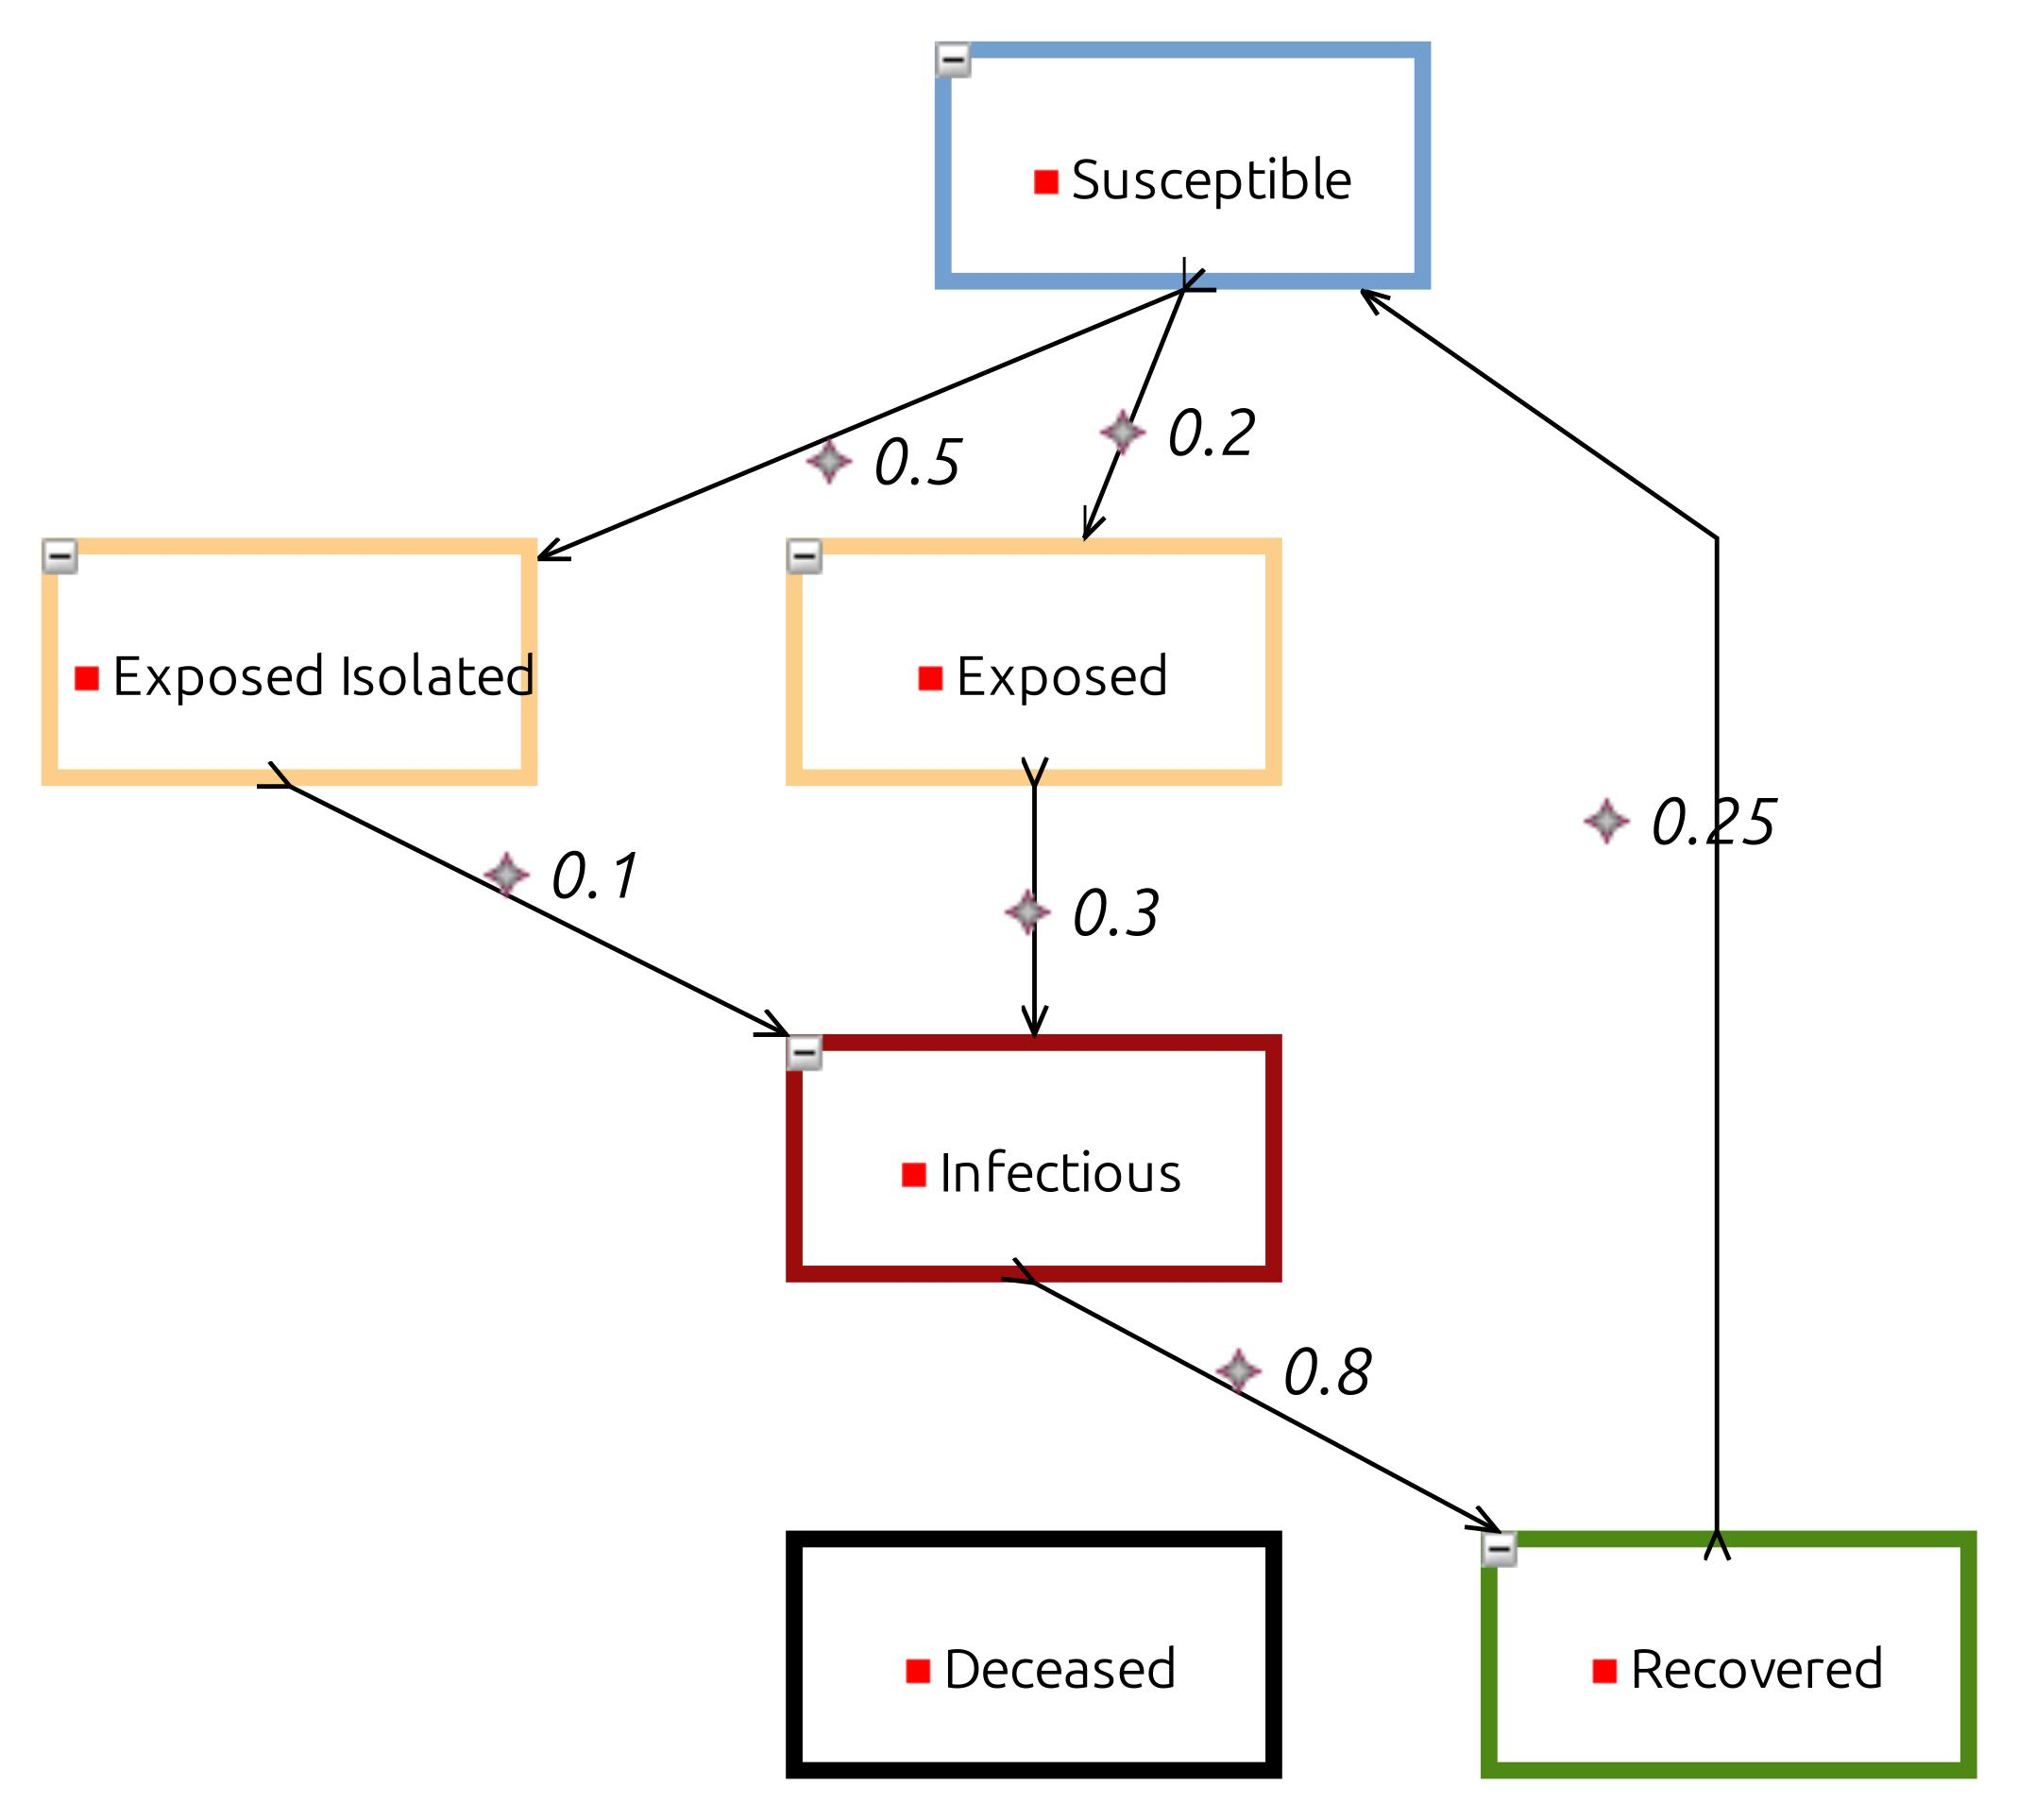
\includegraphics[width=0.5\textwidth]{Figures/fig9.jpg}
  \caption{The generated partially completed prototype model in EpiMDE containing Carol's selected features.}
  \label{fig:prototype_result_model}
\end{figure}

% \subsection{Discussion and Future Work}






\section{Discussion: Synthesis Across Case Studies}
\label{sec:discussion}
The three case studies presented in the previous section provide complementary perspectives on the EpiMDE platform's capabilities, limitations, and applicability across different epidemiological modeling scenarios. This discussion synthesizes the key insights from these studies, addressing questions of generality, usability, and platform maturity.

\subsection{Key Insights and Comparison between HIV and COVID-19 Modeling}

The HIV case study provides several important insights that distinguish it from the COVID-19 case study and demonstrate EpiMDE's broader applicability. First, \textbf{behavioral stratification} differs fundamentally from demographic stratification. While COVID-19 models typically stratify by age and comorbidity (biologically determined characteristics), HIV modeling requires stratification by sexual behavior, which involves complex social and behavioral factors. EpiMDE's Group and Product mechanisms handle both types of stratification uniformly, demonstrating the generality of the approach.

Second, \textbf{heterogeneous contact patterns} are more critical in HIV than in COVID-19. HIV transmission rates vary dramatically between population groups (e.g., homosexual men have higher transmission rates than heterosexual populations), and cross-group transmission is asymmetric (e.g., transmission from homosexual men to women occurs, but not vice versa within the same epidemiological context). EpiMDE's StratumSpecificRate feature was essential for capturing this heterogeneity, allowing different transmission rates for each ContactFlow depending on both the source and target strata.

Third, \textbf{chronic disease dynamics} differ from acute infectious diseases. HIV involves long-term treatment states (Treated with ART) and progressive disease stages (Living with AIDS) that do not appear in typical acute disease models like COVID-19. The model also incorporates demographic recruitment (ExternalSources) representing ongoing entry into sexually active populations, which is less relevant for short-term epidemic modeling but critical for endemic diseases studied over decades.

Fourth, the HIV case study validated EpiMDE's \textbf{usability for non-MDE experts}. The model construction required only epidemiological domain knowledge, without requiring understanding of metamodel extensions, wrapper abstractions, or advanced MDE concepts. This confirms that EpiMDE successfully lowers the barrier to entry for epidemiologists while maintaining sufficient expressiveness for complex models.

Finally, the HIV modeling experience revealed that EpiMDE is particularly well-suited for \textbf{diseases with established, stable dynamics}. Unlike COVID-19, which required frequent model updates as new variants and interventions emerged, HIV transmission dynamics are relatively stable. This suggests that EpiMDE is ideal for modeling endemic diseases and established epidemics, while the extensible metamodel may be more appropriate for rapidly evolving diseases requiring frequent structural modifications.

\subsection{Key Insights on the Rapid Prototyping workflow}
This example is not intended as a validated workflow or method, but as a stress test of the platform’s extensibility. Our illustrative example shows that EpiMDE is a viable platform on which to develop  domain-specific modeling workflows, such as interactive rapid prototyping.
This is due to its extensible architecture and appropriate metamodel, using the infrastructure of the Eclipse Modeling Framework. Overall, we are able to confirm the core assumption of MDE: that general-purpose model engineering platforms, when tailored appropriately, can provide significant value in high-stakes domains like epidemiology. 

The example further illuminates some actionable limitations in EpiMDE.
One challenge lies in preparing existing models for use with EpiMDE. 
At present, users must manually reformat their models to conform to the EpiMDE metamodel. 
This is a nontrivial and error-prone task, that can be a significant barrier to using a domain-specific workflow like rapid prototyping. 
However, as EpiMDE is built on the Eclipse Modeling Framework, 
it is well-suited to  leverage model transformations to automate this process. 


Another challenge we identified lies in the platform’s limited support for semantic distinctions across several steps of the workflow.
Currently, our tooling identifies variation points through exact identifier string matching. This  fails to capture semantically equivalent elements, e.g., compartments labeled $S$ and $Susceptible$ are treated as distinct, despite referring to the same epidemiological concept.
Similarly, its clustering mechanisms are based on structural co-occurrence, without regard to the conceptual roles of model elements. 
For example, we do not identify that each input model represents infectious populations differently, and we depend on interactive input for the user to add the appropriate logical relationships.
The detection of logical dependencies between features is also syntactic, flagging structural inconsistencies (e.g., disconnected flows) but missing domain-specific conflicts, such as including both asymptomatic transmission and severe hospitalization without intermediate transitions.
These limitations point to an opportunity to enrich the platform’s semantic processing capabilities.
Future work can explore tighter integration of EpiMDE with Natural Language Processing techniques and Large Language Models, to enable more flexible variation point matching, more coherent clustering, and the identification of plausible feature combinations based on domain knowledge.
This would reduce the manual burden on users and improve the quality and relevance of generated model prototypes.

%\textbf{Limitations in Variation Point Identification: }In step 1 of our approach,  variation point IDs for model elements rely on exact matches of element properties. While this approach simplifies comparison, it misses semantically equivalent elements. For example, variation points for compartments are solely based on compartment names. This could treat compartments named $S$ and $Susceptible$ as distinct variation points, even though they likely represent the same epidemiological concept.
%To address this limitation, future work could use the descriptions that often accompany compartments and apply natural language processing (NLP) techniques to recognize similarities in meaning rather than exact term matching.

%\textbf{Lack of Semantic Refinement in Clustering: }The clusters created using Formal Concept Analysis (FCA) in step 2 are purely structural and only based on the co-occurrence of variation points across models. However, considering the underlying meaning of the elements could avoid clusters with semantically unrelated elements.
%Although we offer an interactive step for the epidemiologist to refine the clusters, a future improvement could design an additional step of semantic refinement before presenting the clusters to the user. This refinement could consider the names, descriptions, and context of the variation points to reorganize clusters to be more coherent.

%\textbf{Limited Detection of Semantic Dependencies: }The automatically identified logical dependencies between features in step 3 are limited to syntactic relationships, such as conflicting flows or missing source and target compartments. While this captures many important constraints, epidemiologists must still manually add semantic or domain-specific dependencies. Future work could streamline users' work by integrating natural language processing techniques to detect potential semantic conflicts or unlikely feature combinations. For instance, if one feature models asymptomatic transmission while another models hospitalization due to severe symptoms, it may be unlikely or illogical for an epidemiologist to include both in the same prototype model. 

\subsection{Key Insights on the LLM-based Automated Model Generation}

\paragraph{Shared Challenges} Both models struggled with \textbf{indexing errors}—incorrect 0-based indices in flow references (e.g., \texttt{target="//@compartments.X"}). The EpiMDE metamodel requires precise numerical tracking across dozens of elements, a task that strains current LLMs' symbolic reference capabilities despite their strong semantic understanding. This represents a fundamental limitation: LLMs excel at pattern matching and natural language understanding but struggle with precise bookkeeping of numerical relationships across large structured outputs.

\paragraph{Stage 3 Robustness} Both models achieved 100\% execution success for simulation script generation (Stage 3) across both case studies. The two-phase skeleton approach—pre-writing universal components (imports, loop structure, plotting) and narrowly scoping LLM responsibilities to ODE transcription—successfully isolated code generation from the error-prone aspects of XML generation. This validates task decomposition as an effective design pattern for LLM-based scientific code generation.

\paragraph{Implications} The cross-model comparison demonstrates that no single LLM currently provides uniformly superior performance. However, several insights emerge. First, \textbf{frontier model access is critical}: Gemini's perfect COVID-19 generation versus GPT-4o's 65\% recall strongly suggests that complex epidemiological model generation requires state-of-the-art capabilities. As models grow in complexity, access to cutting-edge LLMs transitions from optional to necessary. Second, \textbf{error mode complementarity}: Gemini's perfect recall with imperfect precision (hallucinations) is arguably preferable to GPT-4o's imperfect recall (omissions), as false positives are easier to detect and correct in post-processing than false negatives. Validation layers can flag unexpected attributes, but cannot identify missing flows without ground truth comparison. Third, \textbf{indexing requires targeted intervention}: Since both models struggle with numerical reference tracking, prompt engineering alone may be insufficient. Post-processing validation (checking reference consistency) or intermediate index mapping steps (explicitly documenting element positions before XML generation) are likely necessary complements.

\paragraph{Limitations and Challenges} While the pipeline demonstrates substantial promise, several limitations warrant discussion. First, \textbf{validation overhead}: LLM outputs require careful validation, particularly for complex models where omissions or hallucinations can silently corrupt model semantics. The pipeline is best viewed as an assistive technology accelerating modeling rather than a fully autonomous system. Second, \textbf{prompt brittleness}: Performance depends heavily on prompt structure and clarity. The COVID-19 flow omission pattern in GPT-4o suggests that even clear user specifications can be ambiguous to LLMs if prompt instructions for translating descriptions into XML are insufficiently explicit. Third, \textbf{semantic verification gaps}: The pipeline enforces structural constraints (valid XML, correct element nesting) but cannot detect epidemiologically implausible parameter values or logically invalid model structures (e.g., transmission without contact, recovery before infection). Domain expertise remains essential for semantic validation. Fourth, \textbf{scalability uncertainty}: While Gemini handled the 63-element COVID-19 model perfectly, we have not yet tested models with hundreds of compartments or dozens of stratification dimensions. Performance degradation at extreme scales remains possible.

\subsection{Key Insights on the EpiMDE Modeling Platform}

\paragraph{Accessibility and Immediate Usability}

A central design goal of EpiMDELite was to provide immediate usability for epidemiologists without requiring MDE expertise. The HIV and COVID-19 case studies validate this goal. Both studies successfully replicated published mathematical models, producing simulation results identical to the original publications. The HIV case study, in particular, demonstrated that epidemiologists can leverage EpiMDELite's stratification features (Groups, Products, StratumSpecificRate) without understanding the underlying metamodel mechanics. The ability to define a single Group for "SexualBehavior" and automatically expand compartments across three demographic strata represents a significant reduction in manual effort compared to traditional tools like IDM-CMS or Matlab, where modelers must manually write equations for each stratified compartment.

However, the rapid prototyping case study revealed a current limitation in accessibility: preparing existing models for use with EpiMDE requires manual reformatting to conform to the metamodel. This creates a barrier to entry when epidemiologists want to import legacy models or models from collaborators. While model transformation techniques can address this limitation, the current manual process highlights that accessibility is not yet complete across all platform workflows.

\paragraph{Stratification as a First-Class Concept}

Population stratification emerged as a critical differentiator across the case studies. The HIV model required behavioral stratification (sexual behavior), while the COVID-19 model required demographic stratification (age, comorbidity). EpiMDELite's unified approach to stratification through Groups and Products handled both cases uniformly, despite their conceptual differences. This contrasts with traditional approaches where demographic stratification might be handled through explicit compartment multiplication, while behavioral stratification requires careful consideration of contact patterns.

The COVID-19 study further highlighted the value of explicit stratification representation. The original Tuite et al. model stratified by 16 age groups and comorbidity status, but this stratification was "invisible" in the graphical representation and only appeared in the equations. EpiMDE makes stratification explicit in the model structure, improving transparency and maintainability. This explicitness also facilitated model validation, as the stratification structure was immediately apparent rather than buried in mathematical notation.

\paragraph{Disease Characteristics and Metamodel Selection}

The case studies revealed important insights about when to use EpiMDELite versus the extensible metamodel. EpiMDELite proved well-suited for diseases with established, stable dynamics (HIV) where the core model structure is unlikely to change frequently. For such diseases, the simplified metamodel's constraints are not limiting, and its accessibility benefits dominate.

In contrast, the COVID-19 study demonstrated scenarios where the extensible metamodel's additional capabilities become valuable. COVID-19's rapid evolution (new variants, changing interventions) requires frequent model restructuring. The extensible metamodel's wrapper-based abstractions and compositional features (e.g., Groups within Products, Link compartments) enable modular model evolution. For instance, adding isolation status as a new dimension or incorporating hospitalization dynamics could be done through metamodel extensions without restructuring the entire model.

This suggests a maturity progression: epidemiologists can begin with EpiMDELite for initial model development and validation, then transition to the extensible metamodel when their modeling needs require more sophisticated structural manipulation.

\paragraph{Reproducibility and Model Sharing}

The first three case studies emphasized reproducibility challenges in current epidemiological practice. The COVID-19 study explicitly noted that critical model information was only available in the source code repository, not the published manuscript. The rapid prototyping study addressed this through systematic model reuse, but revealed that semantic matching (e.g., recognizing that "S" and "Susceptible" refer to the same concept) remains a manual task.

EpiMDE improves reproducibility through several mechanisms. First, graphical model representations serve as executable documentation, capturing both structure and semantics in a single artifact. Second, automatic equation generation eliminates transcription errors that plague manual equation implementation. Third, the platform's model differencing capabilities (demonstrated in the COVID-19 validation) enable systematic comparison between models, facilitating validation and knowledge transfer between research groups.

However, the rapid prototyping study identified an important gap: while EpiMDE facilitates reuse within the platform, importing models from external sources (e.g., published papers, other tools) remains manual. Future integration with model transformation frameworks could address this by providing automated translation from common epidemiological modeling formats.

\paragraph{Validation and Correctness}

Model validation emerged as both a strength and an opportunity for improvement. The HIV and COVID-19 studies demonstrated that EpiMDE-generated simulations match published results exactly, validating the platform's correctness. The COVID-19 study's validation approach (comparing derivatives over randomly generated population distributions) provides a systematic method for verifying model equivalence.

However, the rapid prototyping study revealed limitations in semantic validation. The platform detects structural inconsistencies (e.g., flows with missing source/target compartments) but cannot identify domain-specific logical errors (e.g., modeling asymptomatic transmission alongside severe hospitalization without intermediate states). While metamodel constraints prevent many errors at design time, richer domain-specific validation rules could further improve model quality.

\paragraph{Platform Extensibility and Workflow Support}

The rapid prototyping case study demonstrates that EpiMDE's infrastructure (built on EMF and Eclipse) supports the development of domain-specific workflows beyond basic modeling. The four-step rapid prototyping workflow (variation point extraction, feature identification, relationship identification, prototype generation) was implemented as an extension of the platform without modifying the core metamodel or tooling.

This extensibility validates the MDE approach's core assumption: that general-purpose model engineering platforms, when appropriately tailored, can provide significant value in specialized domains. However, the study also revealed friction points. The reliance on exact string matching for variation point identification and purely structural clustering limits semantic reasoning. Future integration with natural language processing or large language models could enhance semantic capabilities while maintaining the platform's structural rigor.

\paragraph{Automation and AI-Assisted Modeling}

Rather than simplifying the modeling interface, the LLM pipeline eliminates the need to use it for initial model creation. This represents an important evolution in making MDE accessible to domain experts: instead of training users on metamodels and graphical editors, the system accepts specifications in formats already familiar to epidemiologists (textual descriptions with mathematical notation).

The multi-stage pipeline architecture (structural generation, value mapping, simulation synthesis) demonstrates that LLMs can serve as effective translators between domain-specific natural language and formal metamodel-compliant representations. The key insight is constraining LLM behavior through structured prompts and explicit validation stages rather than relying on end-to-end generation. This design acknowledges LLM limitations (potential for hallucination, difficulty with precise syntax) while leveraging their strengths (understanding natural language, pattern recognition in mathematical notation).

The LLM pipeline complements rather than replaces the graphical IDE. Models generated automatically can be visualized, validated, and refined graphically. This hybrid workflow accommodates different user preferences and modeling scenarios: textual specifications for reproducing published models, graphical editing for exploratory modeling and composition. The case study highlights that accessibility in MDE should be viewed as a spectrum of interaction modalities rather than a single "best" interface.

However, the LLM approach also introduces new challenges. Validation becomes more critical when models are generated automatically, as users may not immediately understand the resulting structure. The pipeline's reliance on careful prompt engineering means that robustness depends on anticipating potential failure modes. Future work should explore interactive validation workflows where LLMs explain their generated models to users, enabling collaborative refinement rather than one-shot generation.

\paragraph{Comparison to Traditional Approaches}

Across all case studies, EpiMDE demonstrated advantages over traditional epidemiological modeling tools. Compared to tools like STEM (complex, crash-prone interface) or IDM-CMS (hundreds of lines of manual equation writing), EpiMDE's graphical modeling and automatic equation generation significantly reduce cognitive load and development time. The HIV model, which would require separate equations for each of 15 stratified compartments (5 disease states × 3 behavioral groups) in traditional tools, was constructed using a single Product definition in EpiMDE.

However, traditional tools retain advantages in specific areas. Tools like Matlab offer greater flexibility for non-standard model structures, while R-based tools like EpiModel provide extensive statistical analysis capabilities that EpiMDE currently lacks. EpiMDE's value proposition is strongest when model structure, stratification, and reproducibility are primary concerns, rather than statistical inference or highly customized dynamics.

\paragraph{Implications for MDE in Scientific Computing}

The case studies provide broader lessons for applying MDE in scientific computing domains. First, accessibility cannot be assumed even when using domain-familiar concepts. The manual reformatting required for legacy models highlights that interoperability with existing ecosystems is critical for adoption. The LLM pipeline addresses this by accepting natural language specifications, demonstrating that AI-assisted transformation can bridge the gap between traditional scientific workflows and formal metamodeling.

Second, metamodel design involves fundamental trade-offs between simplicity and expressiveness. EpiMDELite's success in the HIV study and the extensible metamodel's value in COVID-19 modeling suggest that offering both options, with clear guidance on when to use each, may be more effective than seeking a single "optimal" metamodel. Third, semantic reasoning remains challenging in MDE approaches. While metamodels excel at capturing structure and enforcing structural constraints, domain-specific semantic validation often requires complementary techniques. The LLM pipeline demonstrates one such complementary approach, though it introduces new validation requirements.

Fourth, the LLM pipeline case study suggests that the future of MDE accessibility may lie in multi-modal interaction rather than finding the "right" interface. Different users and scenarios benefit from different interaction modes: textual specifications for reproducing literature, graphical editing for exploration, programmatic APIs for batch processing. Supporting seamless transitions between these modes may be more valuable than optimizing any single mode.

These insights suggest that successful MDE platforms for scientific domains should prioritize: (1) interoperability with existing tools and formats through automated transformation, (2) layered abstraction with clear migration paths between levels, (3) hybrid approaches combining structural metamodeling with semantic reasoning techniques from AI and natural language processing, and (4) multi-modal interaction supporting diverse user preferences and workflow requirements.


\section{Conclusion}
EpiMDE is an integrated development and modeling environment for epidemiological modeling, addressing key challenges in model sharing, reproducibility, and systematic evolution. In this work, we presented \texttt{EpiMDE-model}, an extensible metamodel that supports both \textbf{basic} modeling for immediate usability through familiar epidemiological concepts (compartments, flows, stratification), but is also \textbf{extensible} with advanced features for sophisticated modeling needs. The \texttt{EpiMDE-model} prioritizes ease of use by providing explicit support for population stratification, external population dynamics (births, deaths, migration), and heterogeneous rates, while avoiding complex abstractions that require MDE expertise.

We demonstrated the EpiMDE platform's effectiveness through four complementary case studies. The COVID-19 and HIV modeling case studies showed that \texttt{EpiMDE-model} produces structurally and functionally equivalent models to published mathematical models while being more concise and accessible, with the HIV case study specifically validating behavioral stratification modeling. The rapid prototyping case study illustrated how model reuse and composition accelerate development. The LLM-based automated generation case study introduced a novel approach to accessibility, demonstrating how AI-assisted transformation can bridge the gap between traditional epidemiological workflows and formal MDE approaches by accepting natural language specifications and producing metamodel-conformant models.

The platform supports multiple interaction modalities—graphical modeling for exploration and composition, and text-based automated generation for reproducing published models—accommodating diverse user preferences and scenarios. The dual-metamodel approach enables a progression path: epidemiologists can start with the basic \texttt{EpiMDE-model} for its accessibility and transition to the extensible version as their needs become more sophisticated. Future work will continue implementing advanced MDE features, including formal model verification, enhanced automatic code generation, improved parameterization support, and refinement of the LLM pipeline with interactive validation workflows and semantic reasoning capabilities.
\label{sec:conclusion}
%%
%% The acknowledgments section is defined using the "acks" environment
%% (and NOT an unnumbered section). This ensures the proper
%% identification of the section in the article metadata, and the
%% consistent spelling of the heading.
\bmhead{Acknowledgements}
The authors would like to thank Dr Simon de Montigny for his invaluable input and experience in epidemiological modeling. 


%%===========================================================================================%%
%% If you are submitting to one of the Nature Portfolio journals, using the eJP submission   %%
%% system, please include the references within the manuscript file itself. You may do this  %%
%% by copying the reference list from your .bbl file, paste it into the main manuscript .tex %%
%% file, and delete the associated \verb+\bibliography+ commands.                            %%
%%===========================================================================================%%

\bibliography{sn-bibliography}% common bib file
%% if required, the content of .bbl file can be included here once bbl is generated
%%\input sn-article.bbl

\appendix
\section{Appendix}
\label{section:appendix}


\begin{table}[ht]
\centering
\begin{tabularx}{\textwidth}{|l|Y|}
\hline
\textbf{Model} & \textbf{Variation Points} \\ \hline
$m_1$ & Susceptible, Vaccinated, Exposed, Exposed\_Isolated, Infectious, Recovered, Susceptible\_Vaccinated\_0.2, Susceptible\_Exposed\_0.2, Susceptible\_Exposed\_Isolated\_0.5, Vaccinated\_Susceptible\_0.3, Exposed\_Infectious\_0.3, Exposed\_Isolated\_Infectious\_0.1, Infectious\_Recovered\_0.8, Recovered\_Susceptible\_0.25 \\ \hline
$m_2$ & Susceptible, Vaccinated, Exposed, Infectious\_Asymptomatic, Infectious\_Moderate\_Symptomatic, Infectious\_Sever\_Symptomatic, Recovered, Deceased, Susceptible\_Vaccinated\_0.2, Susceptible\_Exposed\_0.4, Vaccinated\_Susceptible\_0.3, Exposed\_Infectious\_Asymptomatic\_0.1, Exposed\_Infectious\_Moderate\_Symptomatic\_0.2, Exposed\_Infectious\_Sever\_Symptomatic\_0.4, Infectious\_Asymptomatic\_Recovered\_0.9, Infectious\_Moderate\_Symptomatic\_Recovered\_0.5, Infectious\_Sever\_Symptomatic\_Recovered\_0.2, Infectious\_Sever\_Symptomatic\_Deceased\_0.8\\ \hline
$m_3$ & Susceptible, Exposed, Infectious\_Isolated, Infectious\_NonIsolated, Hospitalized, Hospital\_No\_Access, Recovered, Deceased, Susceptible\_Exposed\_0.5, Exposed\_Infectious\_Isolated\_0.2, Exposed\_Infectious\_NonIsolated\_0.2, Infectious\_Isolated\_Hospitalized\_0.5, Infectious\_Isolated\_Hospital\_No\_Access\_0.3, Hospitalized\_Recovered\_0.8, Hospitalized\_Deceased\_0.2, Hospital\_No\_Access\_Recovered\_0.1, Hospital\_No\_Access\_Deceased\_0.8 \\ \hline

\end{tabularx}
\caption{Identified variation points for each compartmental model. Each row lists the models $m_1$, $m_2$, and $m_3$, along with their corresponding variation point IDs.}
\label{tab:prototype_variation_points}
\end{table}


\begin{table}[ht]
\centering
\begin{tabularx}{\textwidth}{|l|l|Y|}
\hline
\textbf{ClusterIndex} & \textbf{ClusterLabel} & \textbf{Variation Points} \\ \hline
$1$ & Core\_SER & Susceptible, Exposed, Recovered \\ \hline
$2$ & Mortality & Deceased\\ \hline
$3$ & Vaccination & Vaccinated, Susceptible\_Vaccinated\_0.2, Vaccinated\_Susceptible\_0.3 \\ \hline
$4$ & Isolated\_Hospital & Infectious\_Isolated, Infectious\_NonIsolated, Hospitalized, Hospital\_No\_Access, Susceptible\_Exposed\_0.5, Exposed\_Infectious\_Isolated\_0.2, Exposed\_Infectious\_NonIsolated\_0.2, Infectious\_Isolated\_Hospitalized\_0.5, Infectious\_Isolated\_Hospital\_No\_Access\_0.3, Hospitalized\_Recovered\_0.8, Hospitalized\_Deceased\_0.2, Hospital\_No\_Access\_Recovered\_0.1, Hospital\_No\_Access\_Deceased\_0.8
\\ \hline
$5$ & Symptom\_Severity & Infectious\_Asymptomatic, Infectious\_Moderate\_Symptomatic, Infectious\_Sever\_Symptomatic, Susceptible\_Exposed\_0.4, Exposed\_Infectious\_Asymptomatic\_0.1, Exposed\_Infectious\_Moderate\_Symptomatic\_0.2, Exposed\_Infectious\_Sever\_Symptomatic\_0.4, Infectious\_Asymptomatic\_Recovered\_0.9, Infectious\_Moderate\_Symptomatic\_Recovered\_0.5, Infectious\_Sever\_Symptomatic\_Recovered\_0.2, Infectious\_Sever\_Symptomatic\_Deceased\_0.8\\ \hline
$6$ & Exposed\_Isolation\_States & Exposed\_Isolated, Infectious, Susceptible\_Exposed\_0.2, Susceptible\_Exposed\_Isolated\_0.5, Exposed\_Infectious\_0.3, Exposed\_Isolated\_Infectious\_0.1, Infectious\_Recovered\_0.8, Recovered\_Susceptible\_0.25\\ \hline

\end{tabularx}
\caption{Identified clusters and their associated variation points. The labels are assigned by the user. After finalization and labeling, each row is referred to as a \textit{feature}.}
\label{tab:prototype_clusters}
\end{table}

\end{document}